The goal of this analysis is to search for long-lived Heavy Neutral Leptons in the 1-20 GeV mass range. While the displaced vertex driven search provides a clean signature to work with, there are various sources of backgrounds that contaminate the targeted phase space.~\Cref{sec:backgrounds} describes these backgrounds and the kinematic cuts that remove or reduce them.~\Cref{sec:corr_bkg} details the study of the background consisting of DVs with correlated tracks and its method of estimation.~\Cref{sec:uncorr_bkg} outlines the same for DVs with uncorrelated tracks. After all the background estimation methods are in place, the signal strength is extracted using a simultaneous fit across all analysis regions as described in~\cref{sec:sig_ext}.

\section{Backgrounds}\label{sec:backgrounds}
The backgrounds considered in this analysis are categorized into reducible and irreducible. While dedicated cuts are used to completely remove reducible backgrounds with negligible impact to the signal, cuts applied to suppress irreducible backgrounds also affect the signal, with the exact cut value optimized to maximize signal significance.

\subsection{Reducible backgrounds}
\begin{figure}[!ht]
    \centering
     \subfloat[$\gamma\to ee$ conversions]{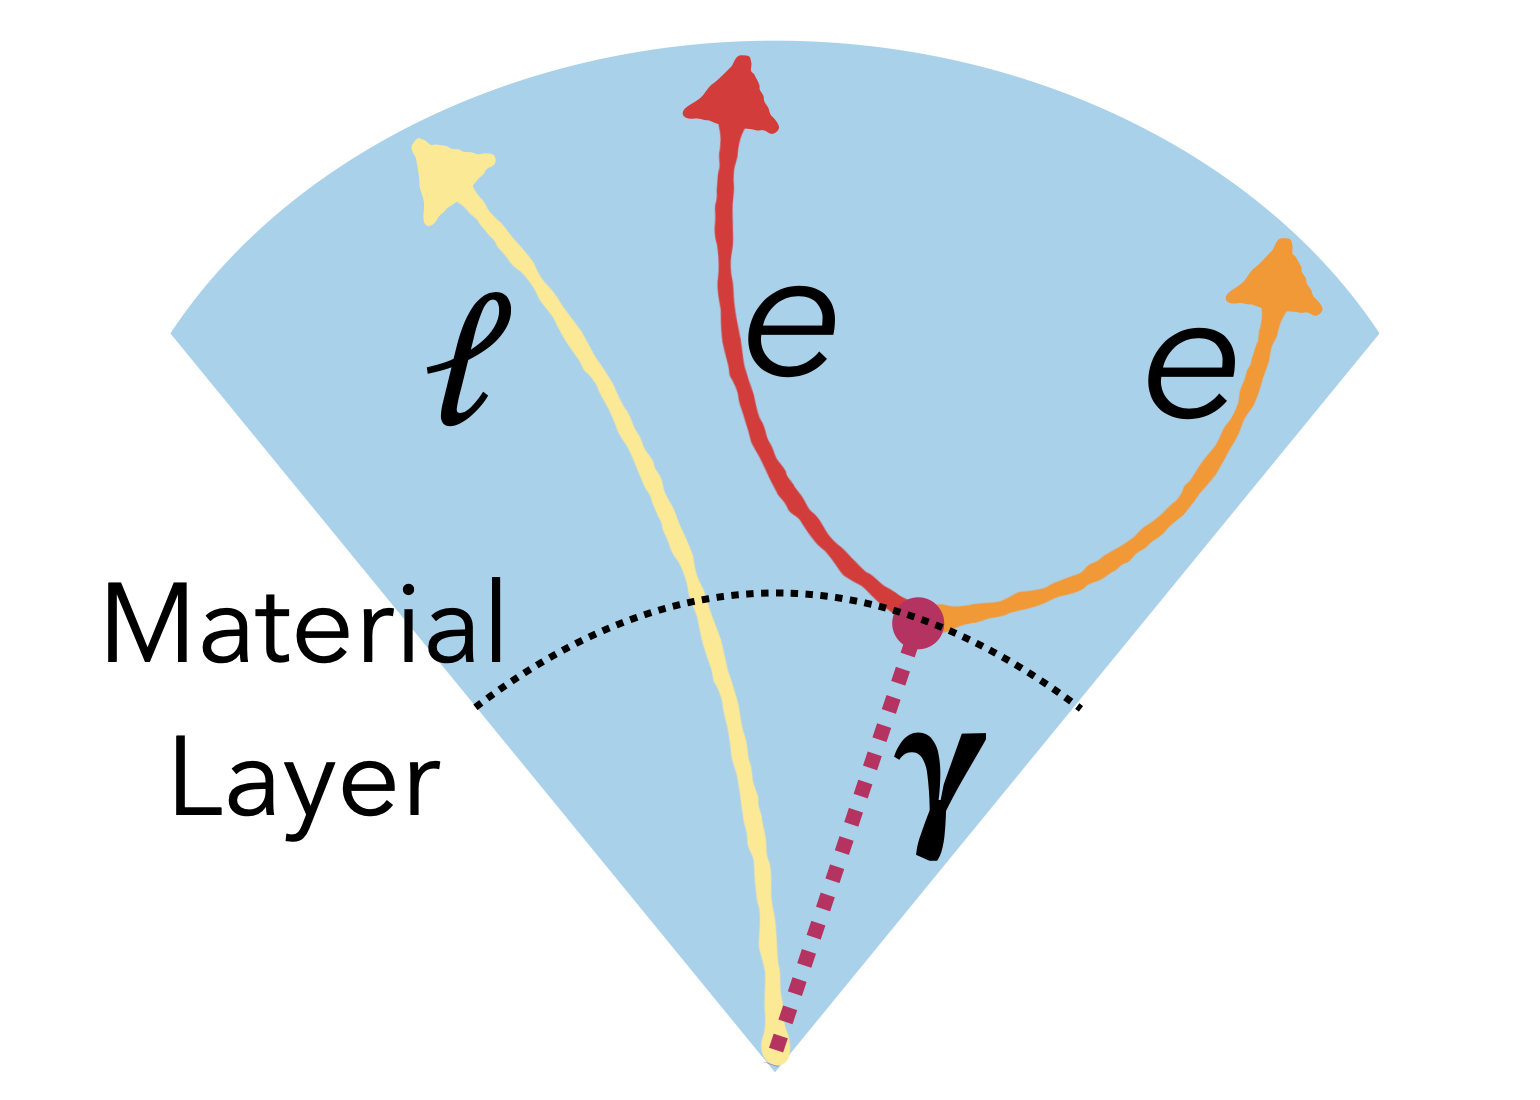
\includegraphics[width=0.3\textwidth]{figures/analysis_strategy/bkg_illustrations/photon_conv.png}}
     \subfloat[Cosmic muons]{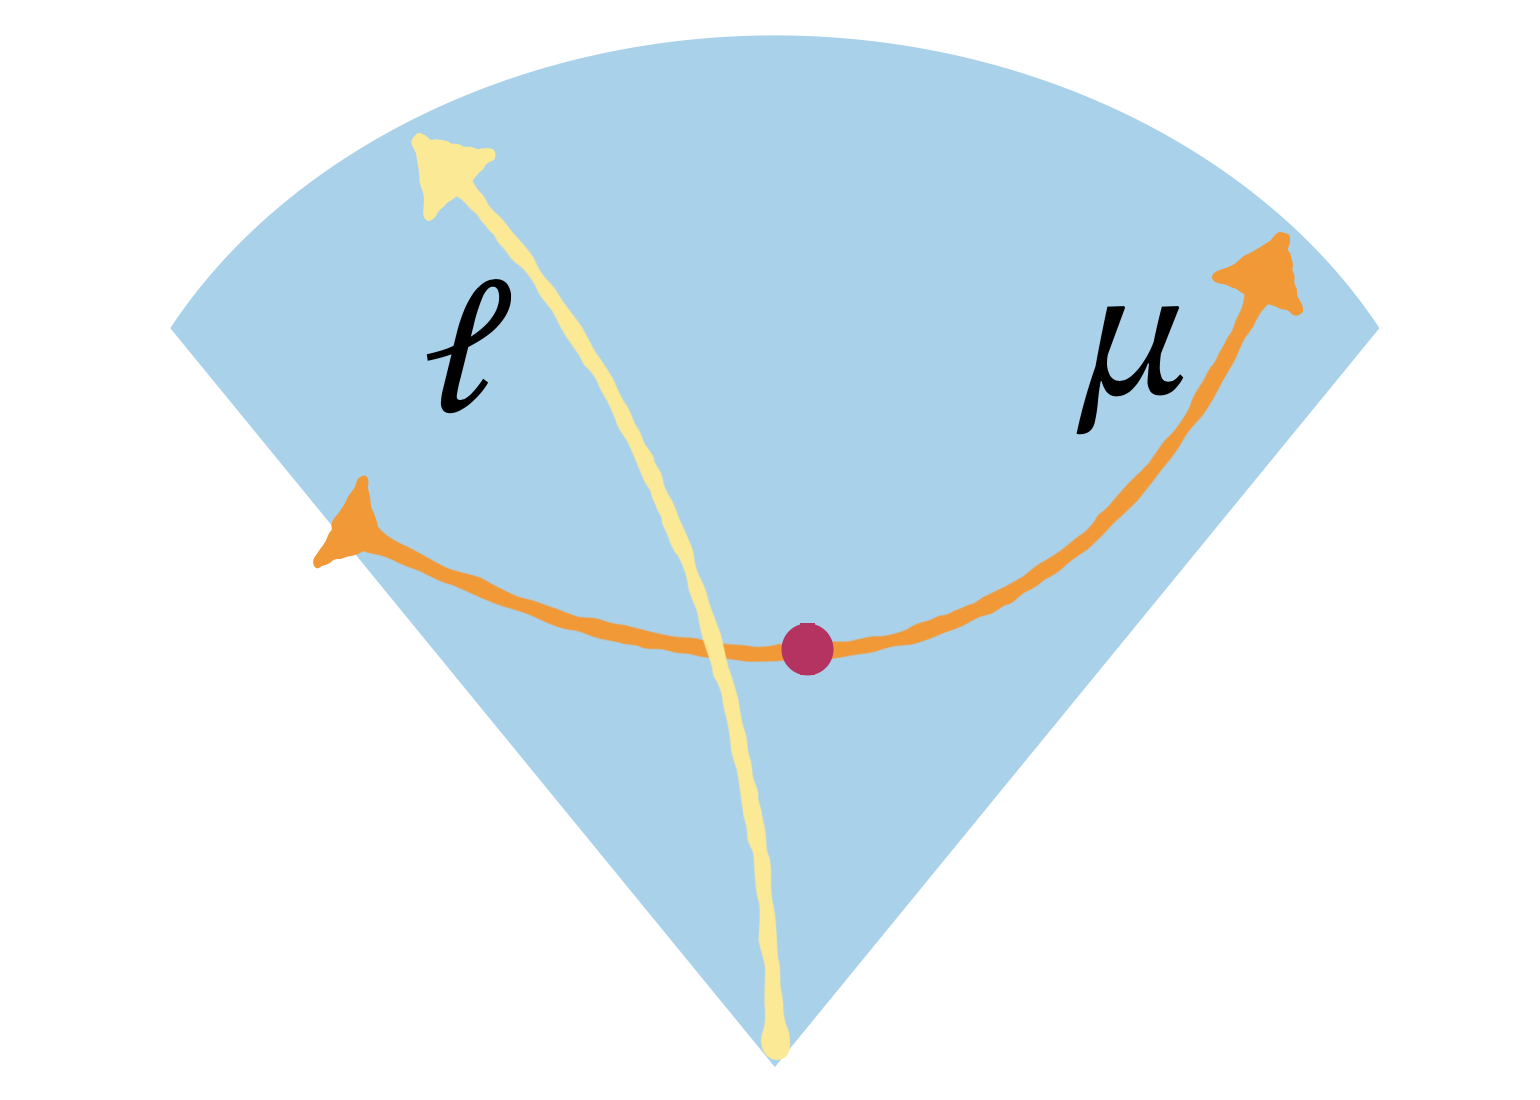
\includegraphics[width=0.3\textwidth]{figures/analysis_strategy/bkg_illustrations/cosmics.png}}
     \subfloat[$Z\to\ell\ell$ decays]{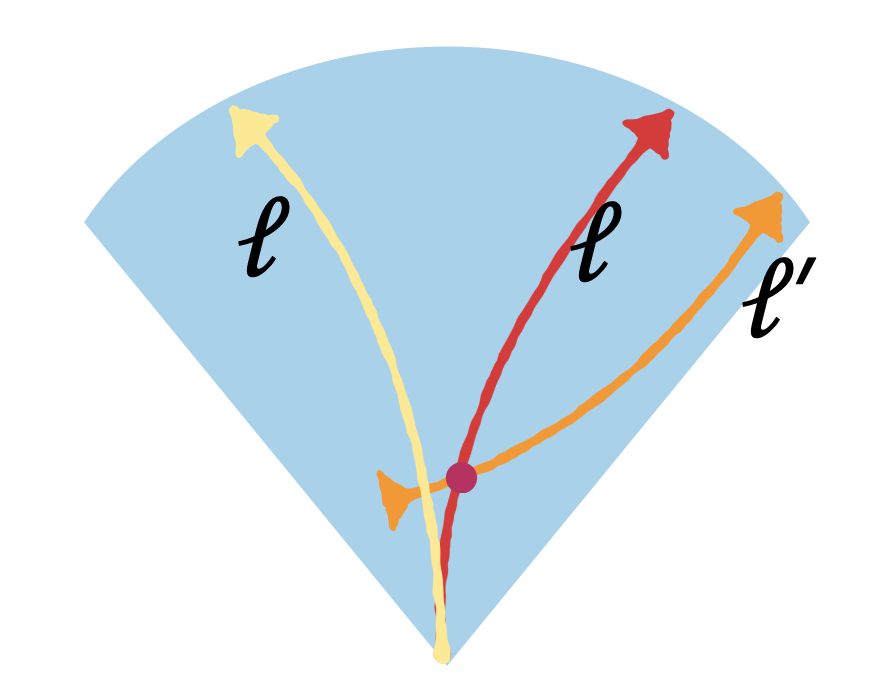
\includegraphics[width=0.3\textwidth]{figures/analysis_strategy/bkg_illustrations/zdecays_1.png}}
     \caption{Illustrative topology of the reducible backgrounds in the ATLAS ID volume.}
     \label{fig:bkg_reducible}
\end{figure}

Three sources of reducible backgrounds affect this analysis, as illustrated in~\cref{fig:bkg_reducible}:
\begin{enumerate}
    \item $\gamma\to ee$ conversions: Photons interacting with the various layers of material in the ID volume recoil against the atoms and produce a $e^+e^-$ pair. Such a $ee$ DV, along with a prompt lepton source, contaminates the measurement phase space. To remove this background, $ee$ DVs are required to be inside a narrower fiducial volume ($|z|<300$~mm) and must satisfy a \textit{material} veto, which rejects DVs which have a reconstructed position consistent with the position of the detector material. The material map, as shown in~\cref{fig:material_map}, is constructed using the known positions of detector elements and from the position of low-mass vertices reconstructed in data~\cite{SUSY-2018-13}. The material veto removes 48\% of the fiducial volume. The two electrons from a photon conversion are highly collinear since the recoiling nucleus takes very little momentum away from the photon. Hence, the \mdv distribution\footnote{$\mdv\approx\sqrt{E_1\cdot E_2 (1-\cos\alpha)+2m_1m_2}$ for relativistic objects with energies and masses $E_1,\,E_2$ and $m_1,\,m_2$, respectively.} starts at $\sqrt{2}m_e$ and falls sharply. Since the \mdv calculation makes a pion mass assumption on the outgoing tracks, the lower mass bound is given by $\sqrt{2}m_{\pi^+}\approx280$~MeV. Hence, to further reject any remaining conversions, a $\mdv>500$~MeV cut is applied on $ee$ DVs. The assumption on the mass does not affect the impact of the cut since an \mdv measurement of the scale $\sqrt{2}m_e$ cannot be resolved by ATLAS. The material veto also hurts the signal efficiency since it removes almost half the fiducial volume from the analysis. However, in the current context, the photon conversion background is still classified as a reducible background since it is completely removed after the above cuts.

    \begin{figure}[!ht]
        \centering
        \subfloat[Positions in $x-y$ plane]{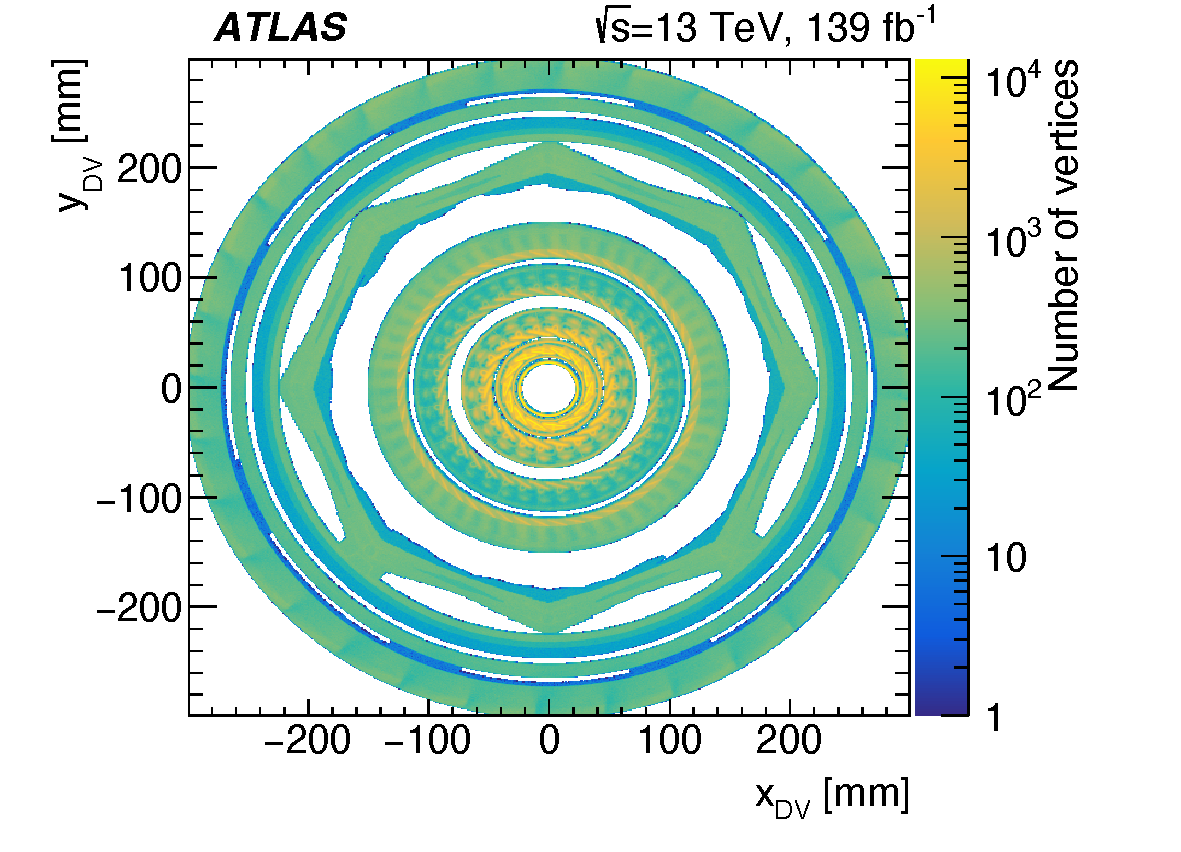
\includegraphics[width=0.5\textwidth]{figures/analysis_strategy/mat_map_xy.pdf}}
        \subfloat[Positions in $r-z$ plane]{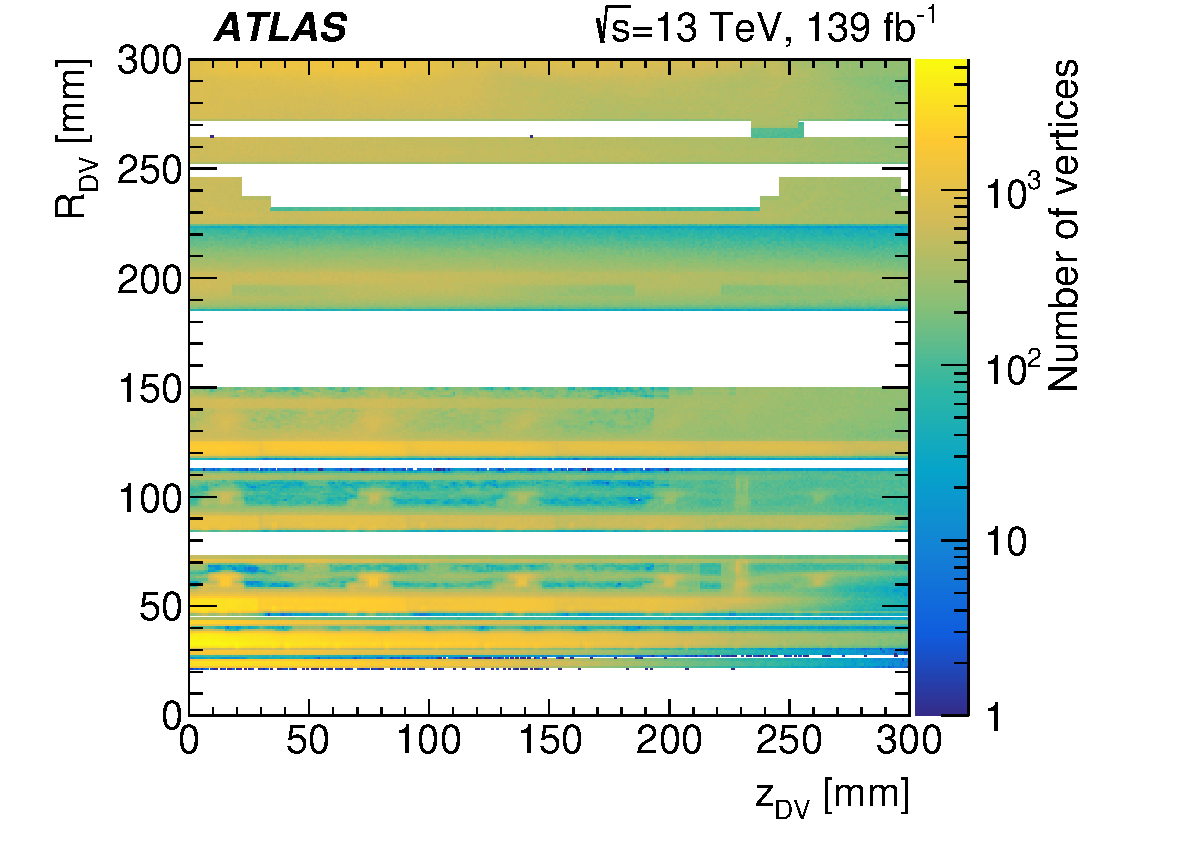
\includegraphics[width=0.5\textwidth]{figures/analysis_strategy/mat_map_rz.pdf}}
        \caption{The positions of reconstructed displaced vertices that are vetoed by the material map.~\cite{SUSY-2018-13}}
        \label{fig:material_map}
    \end{figure}

    \item Cosmic muons: Even though ATLAS is 100 m below the ground, the open shaft above it allows a large flux of muons from the the interaction of cosmic rays with the atmosphere to enter the detector. One such cosmic muon passing through the ATLAS ID can be incorrectly reconstructed as two tracks, with them together reconstructed as the two legs of one secondary vertex. Such a DV is characterized by \textit{back-to-back} tracks i.e. $\eta_\mathrm{track1}\approx-\eta_\mathrm{track2}$ and $\phi_\mathrm{track1}-\phi_\mathrm{track2}\approx\pi$. Hence, a cut on the cosmic separation variable, $\sqrt{(\Sigma_\text{DV tracks}\eta)^2+(\pi-|\Delta_\text{DV tracks}\phi|)^2}>.05$, is applied to reject this background. The exact cut value was optimized for the 2022 analysis, and was found to be sufficient for rejecting all background without affecting signal.

    \item $Z\to\ell\ell$ decays: One of the leptons from a $Z$ decay can be paired with a third uncorrelated lepton to give a lepton+DV topology probed in this analysis. To reject this background, a veto on the $m_{\ell\ell}$ variable around the $Z$ mass, $|m_{\ell\ell}-90\text{ GeV}|>10\text{ GeV}$ is applied to same-flavor opposite-sign (SFOS) pairs of leptons, where one is a prompt lepton and the other is a DV lepton.
\end{enumerate}

~\Cref{tab:cuts_reducible} summarize the cuts applied to reject the three reducible backgrounds that affect this analysis.

\begin{table}[!ht]
    \centering
    \begin{tabular}{cc}
        \hline\hline
         Cut Name & Cut Description\\
         \hline
         Photon Conversions Veto & Material veto applied to $ee$ DVs\\
         Low Mass DV Veto & $\mdv>500$~MeV for $ee$ DVs\\
         Cosmic Muon Veto & $\sqrt{(\Sigma_\text{DV tracks}\eta)^2+(\pi-|\Delta_\text{DV tracks}\phi|)^2}>.05$\\
         $Z\to\ell\ell$ Veto & $|m_{\ell_\mathrm{DV}\ell_\mathrm{prompt}}-90\text{ GeV}|>10\text{ GeV}$ for SFOS pairs \\
         \hline\hline
    \end{tabular}
    \caption{Analysis cuts applied to reject reducible background.}
    \label{tab:cuts_reducible}
\end{table}

\subsection{Irreducible backgrounds}

\begin{figure}[!ht]
    \centering
     \subfloat[Correlated background]{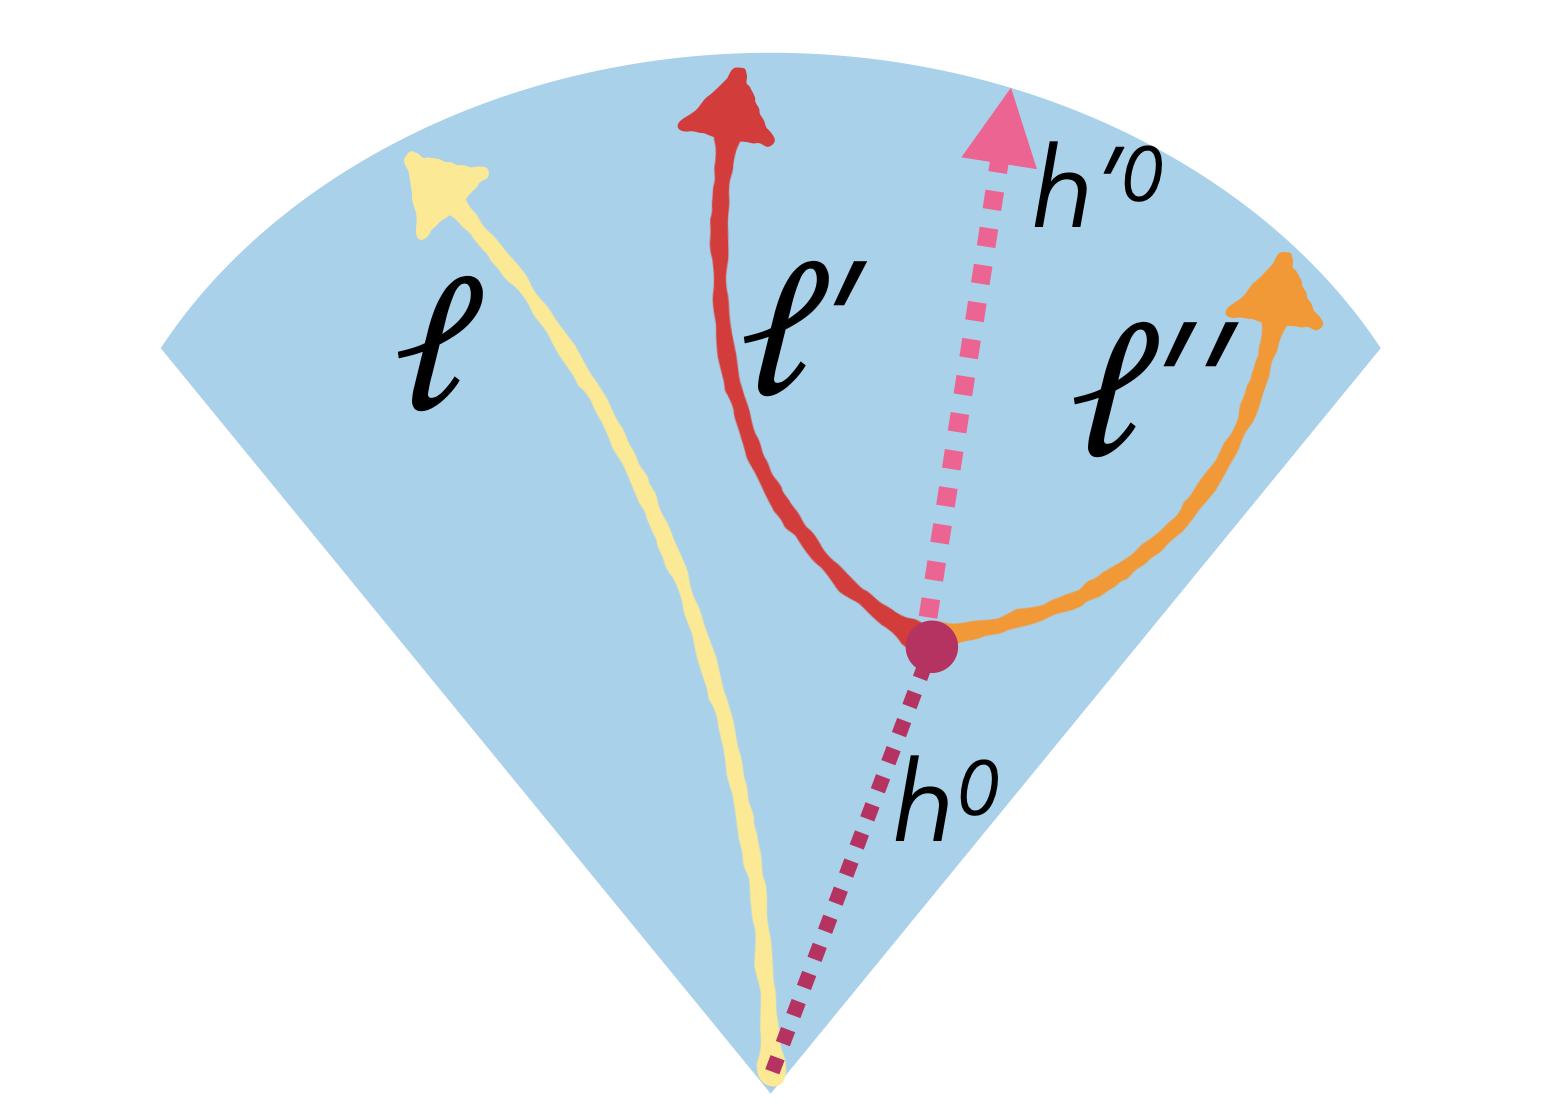
\includegraphics[width=0.4\textwidth]{figures/analysis_strategy/bkg_illustrations/hadrons.png}}
     \subfloat[Uncorrelated background]{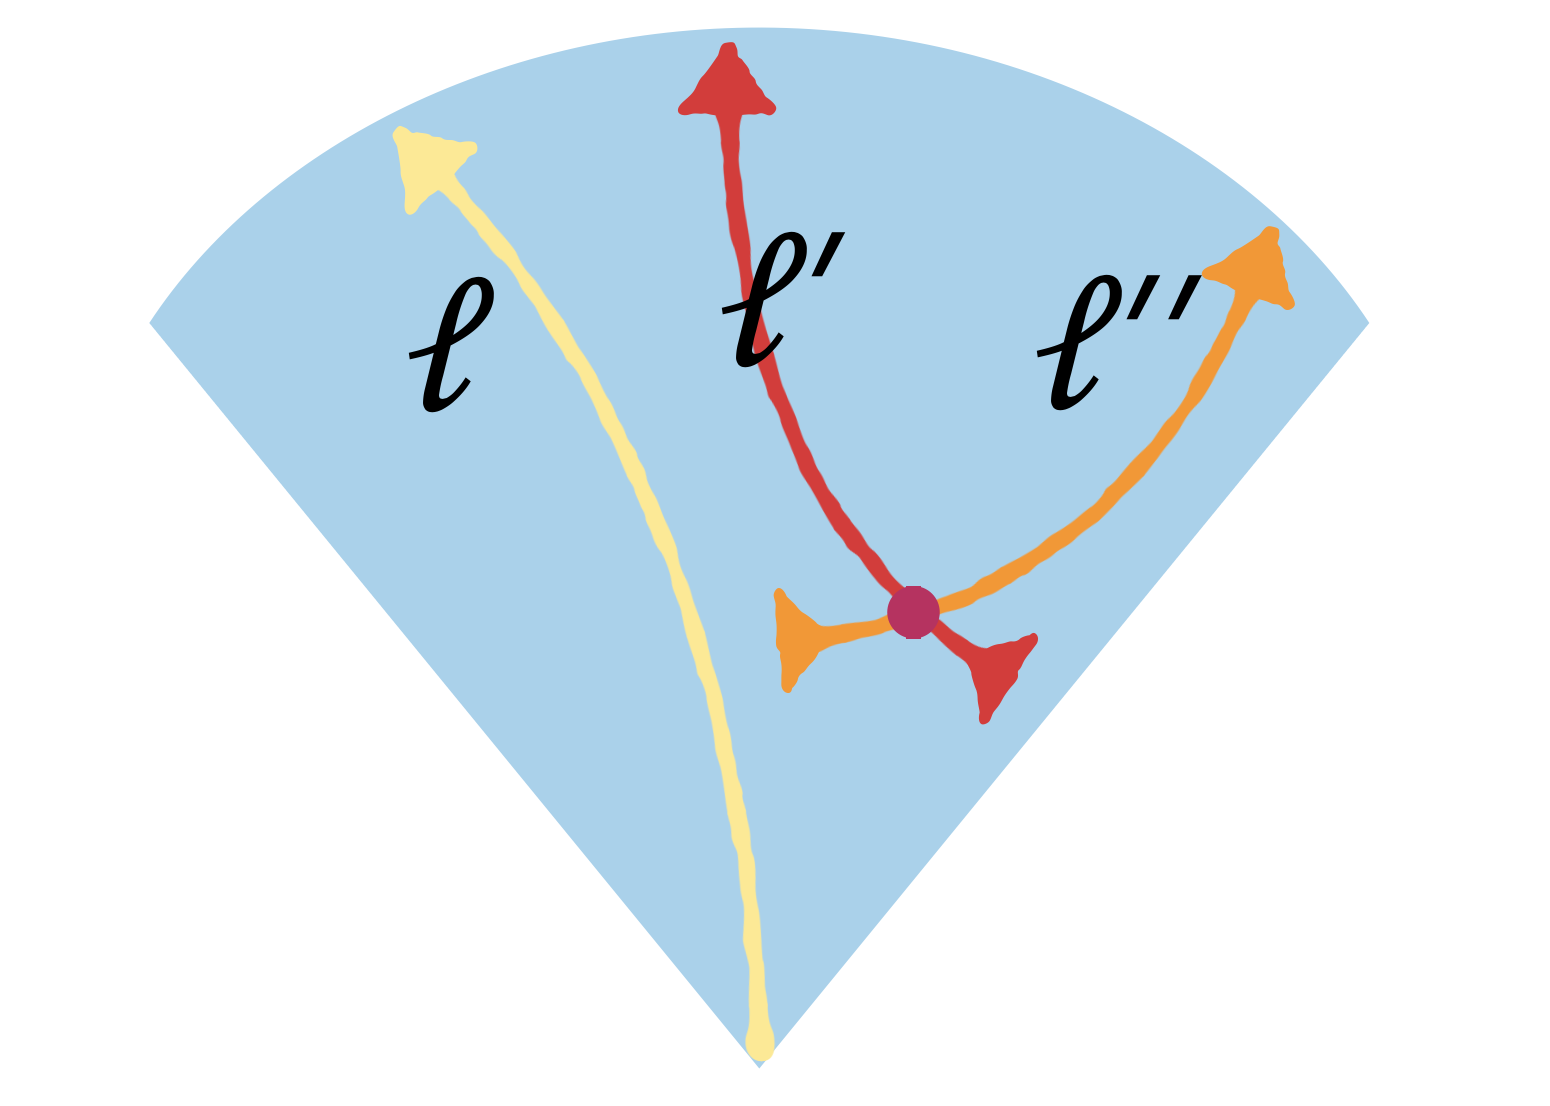
\includegraphics[width=0.4\textwidth]{figures/analysis_strategy/bkg_illustrations/crossings.png}}
     \caption{Illustrative topology of the irreducible backgrounds in the ATLAS ID volume.}
     \label{fig:bkg_irreducible}
\end{figure}

Two sources of irreducible backgrounds affect this analysis, as illustrated in~\cref{fig:bkg_irreducible}:
\begin{enumerate}
    \item Correlated background: The largest background that affects this analysis is the lepton+DV signature coming from correlated decay sources. Heavy hadrons, such as b-hadrons and secondary $J/\psi$, mimic signatures from BSM LLPs and decay macroscopically in the ID volume. While these decays are often multi-legged, two of its legs can be captured by VSI and hence contaminate the phase space targeted in this analysis.~\Cref{sec:corr_bkg} describes the detailed study of this background and the method of its estimation.

    \item Uncorrelated background: A small background contribution comes in the form of uncorrelated track pairs, or \textit{random crossings} (RC), that happen to cross in an event and then captured by VSI. The DV is not a genuine decay but rather an accidental point of crossing.~\Cref{sec:uncorr_bkg} describes the method used in the analysis to estimate the contribution from random crossing background.
\end{enumerate}

\section{Correlated Background}\label{sec:corr_bkg}
As previously stated, the biggest background in this analysis is the background from the production of heavy flavor (HF) hadrons which decay to leptons that are displaced with respect to the primary vertex. These are predominantly found in the \mdv$<5$~GeV phase space. Such a phase space was completely removed from consideration in the 2022 analysis due to the lack of a robust method to estimate them which significantly reduced sensitivity to low mass HNLs. In this analysis, MC simulations of SM processes (specifically of the $t\bar{t}$ and $V+$jets processes) are used to understand and estimate this background. A signal rich phase space, called the Signal Region (SR), is defined to look for HNLs in a wide lifetime-coupling parameter space. A non-overlapping phase space rich in correlated background, called the Heavy Flavor Control Region (HF-CR), is defined to obtain the normalization of this background in a data-driven manner and reduce the uncertainties on the estimate.

\subsection{Analysis regions}

All events considered in this analysis are required to have at least one primary vertex with two tracks with \pT$>500$~MeV. The hard-scatter vertex is selected among all reconstructed primary vertices as the one with the largest $\Sigma\pT^2$, where the sum is over all the tracks attached to the PV.

A pre-selection cut is applied for the selection of signatures from a $W$-decay. The tri-lepton invariant mass ($m_{\ell\ell\ell}$) is used as a proxy for the $W$ mass. Events are required to have 40 GeV$<m_{\ell\ell\ell}<$90 GeV, where the lower cut is more liberal compared to the upper cut to account for energy losses from a neutrino emission. A $J/\psi$-veto is applied for $ee$ and $\mu\mu$ DVs requiring $|\mdv-3.1\text{ GeV}|>0.1\text{ GeV}$.

The final pre-selection cut is applied using a discriminating variable optimized to significantly suppress the contribution from hadron decays. The variable $\mathcal{S}$ is defined as
\begin{equation}
    \mathcal{S}^{2} = {\boldsymbol{\Delta}_{\text{3D}}\text{(PV,DV)}}^T \cdot  {\text{\textbf{Cov}}(\Delta_{\text{3D}(\text{PV,DV})})^{-1}} \cdot {\boldsymbol{\Delta}_{\text{3D}}\text{(PV,DV)}},
\end{equation}
where $\boldsymbol{\Delta}_{\text{3D}}\text{(PV,DV)}$ is the 3D vector of the distance between the primary- and secondary-vertex position, and $\text{\textbf{Cov}}(\Delta_{\text{3D}(\text{PV,DV})})$ is the covariance matrix of the difference between the primary- and secondary-vertex position. $\mathcal{S}$ can be interpreted as a significance of the PV-DV distance. 
%Effectively, this is implemented as follows, defining $\mathcal{W} = \text{Cov}(\Delta_{\text{3D}}(\text{PV,DV}))^{-1}$,
%\begin{equation}
%     \mathcal{S}^{2} = \Delta X^{2} \cdot \mathcal{W}_{00} + \Delta Y^{2} \cdot \mathcal{W}_{11} + \Delta Z^{2} \cdot \mathcal{W}_{22} + 2\Delta X \Delta Y \cdot\mathcal{W}_{01} + 2\Delta X \Delta Z \cdot\mathcal{W}_{02} + 2\Delta Y \Delta Z \cdot\mathcal{W}_{12},
% \end{equation}
%where $\Delta X = \text{PV}_{x} - \text{DV}_{x}$, $\Delta Y$ and $\Delta Z$ are defined in the same way. 
Roughly speaking, DVs with lower values of $\mathcal{S}$ have larger $\pT^\text{DV tracks}$ and lower \rdv and $\Delta R$ between the DV tracks.
 
\begin{figure}[!ht]
    \centering
    \subfloat[Hadron decay background]{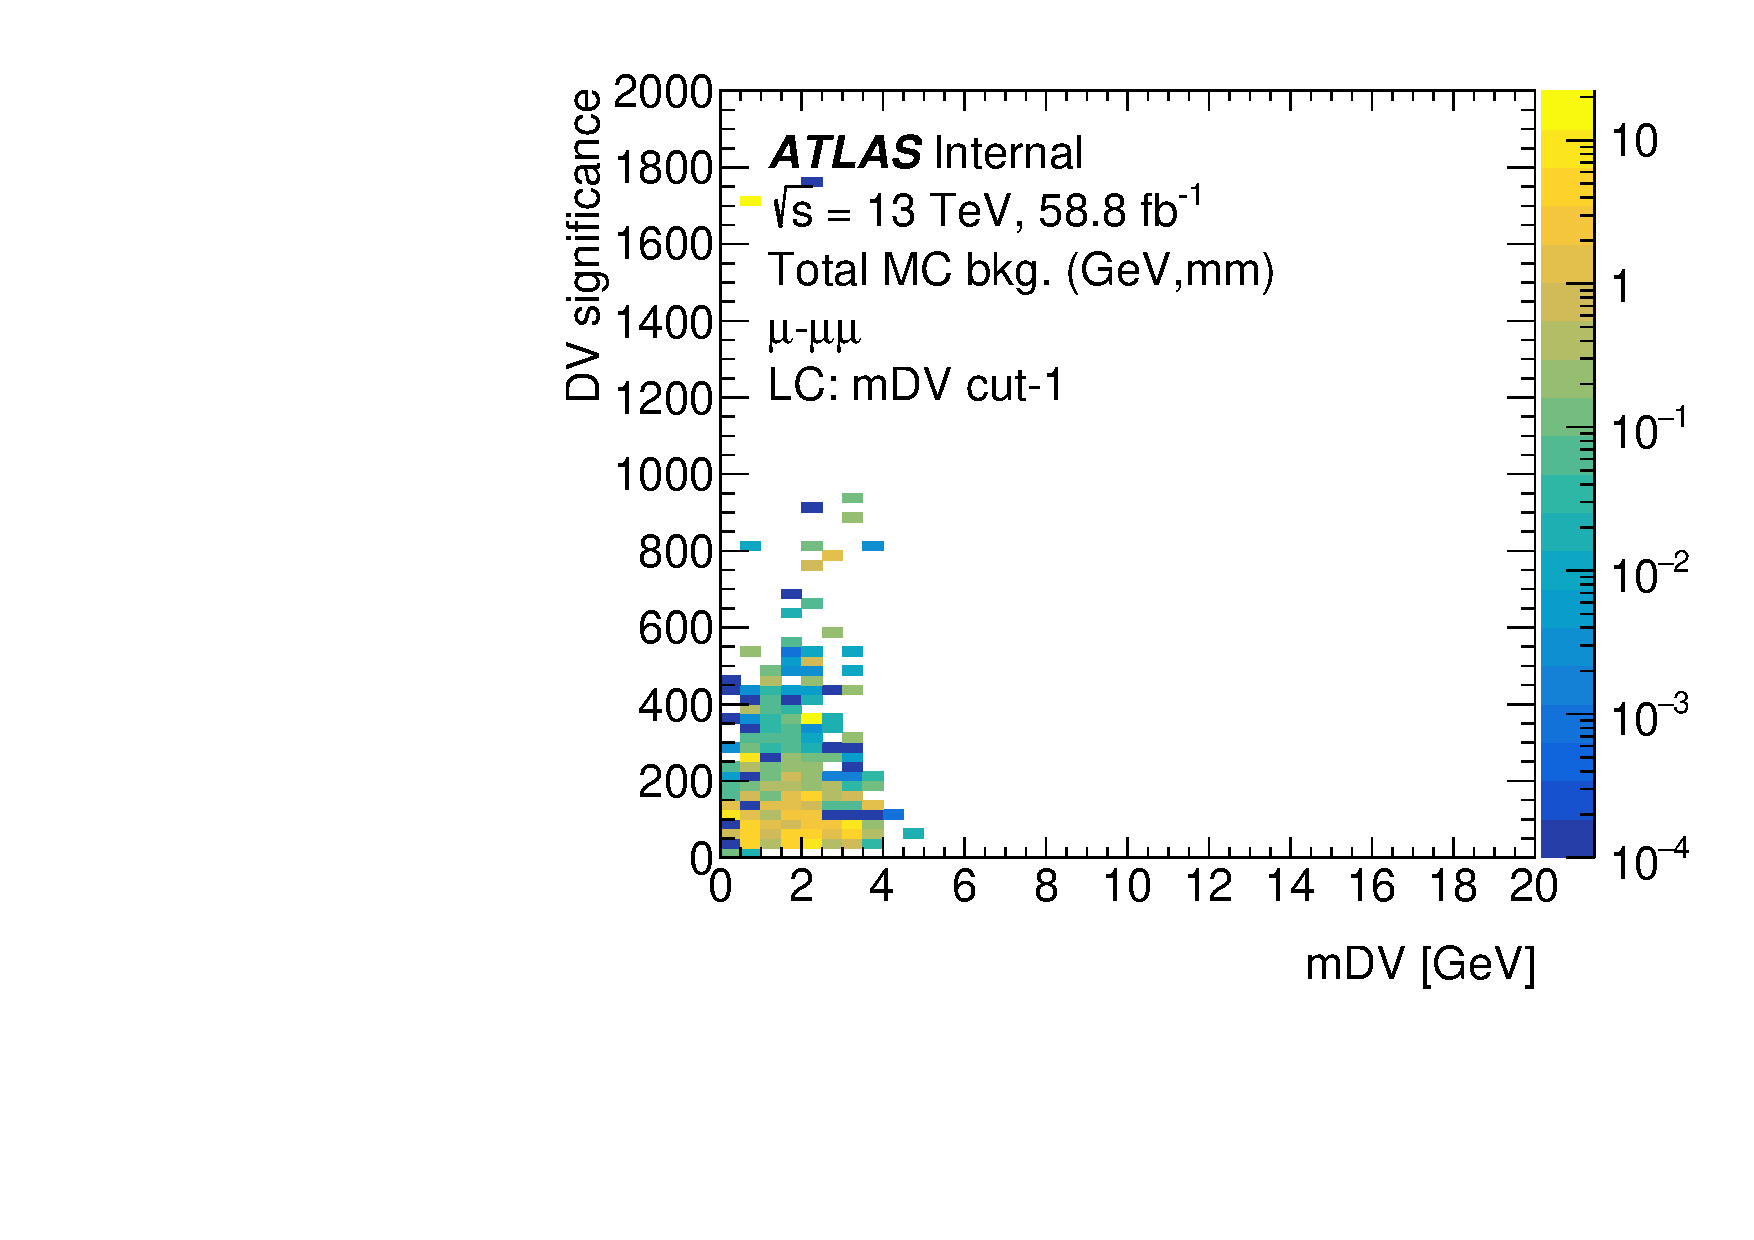
\includegraphics[width=0.45\textwidth]{figures/analysis_strategy/S2D_bkg.pdf}}\\
    \subfloat[\mhnl=2 GeV, \ctau=1000 mm HNL signal]{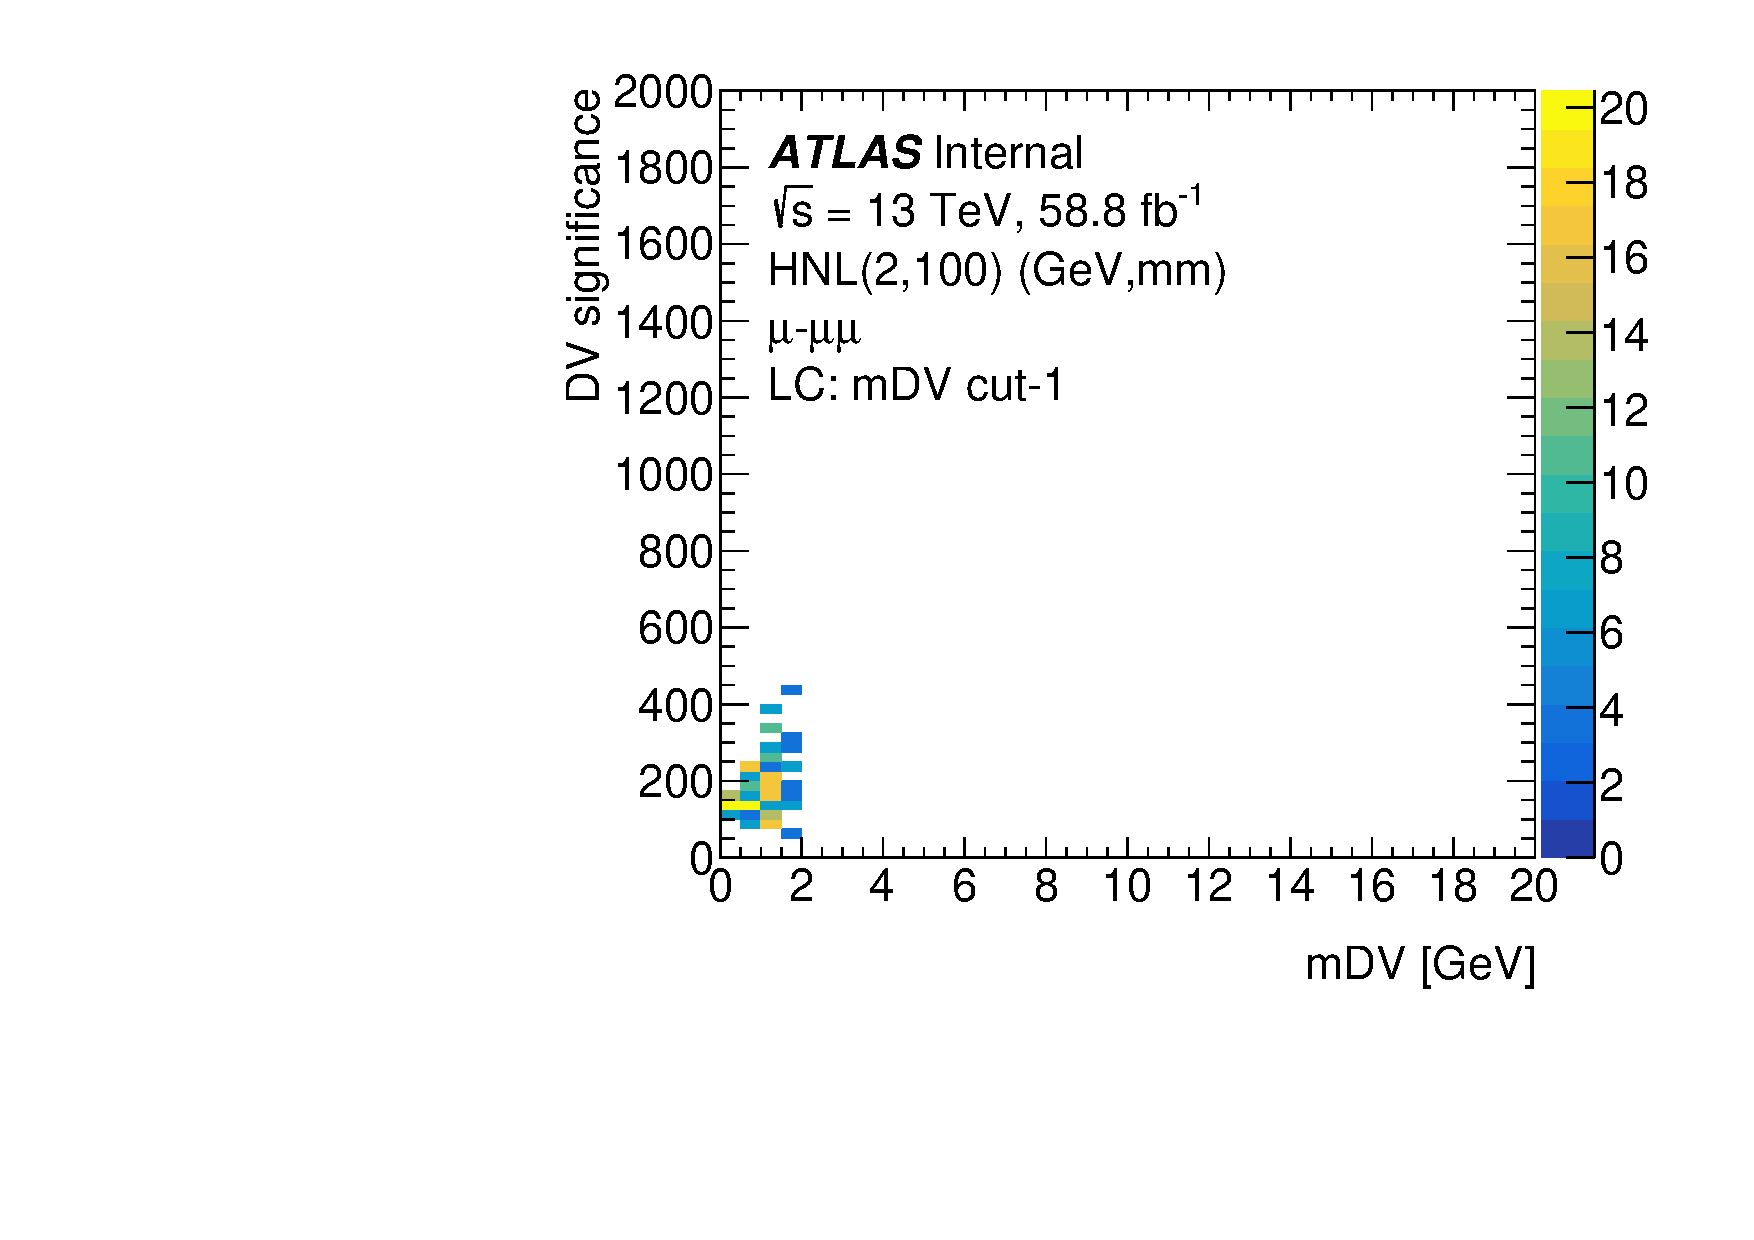
\includegraphics[width=0.45\textwidth]{figures/analysis_strategy/S2D_HNL2_ctau1000.pdf}}
    \subfloat[\mhnl=7.5 GeV, \ctau=100 mm HNL signal]{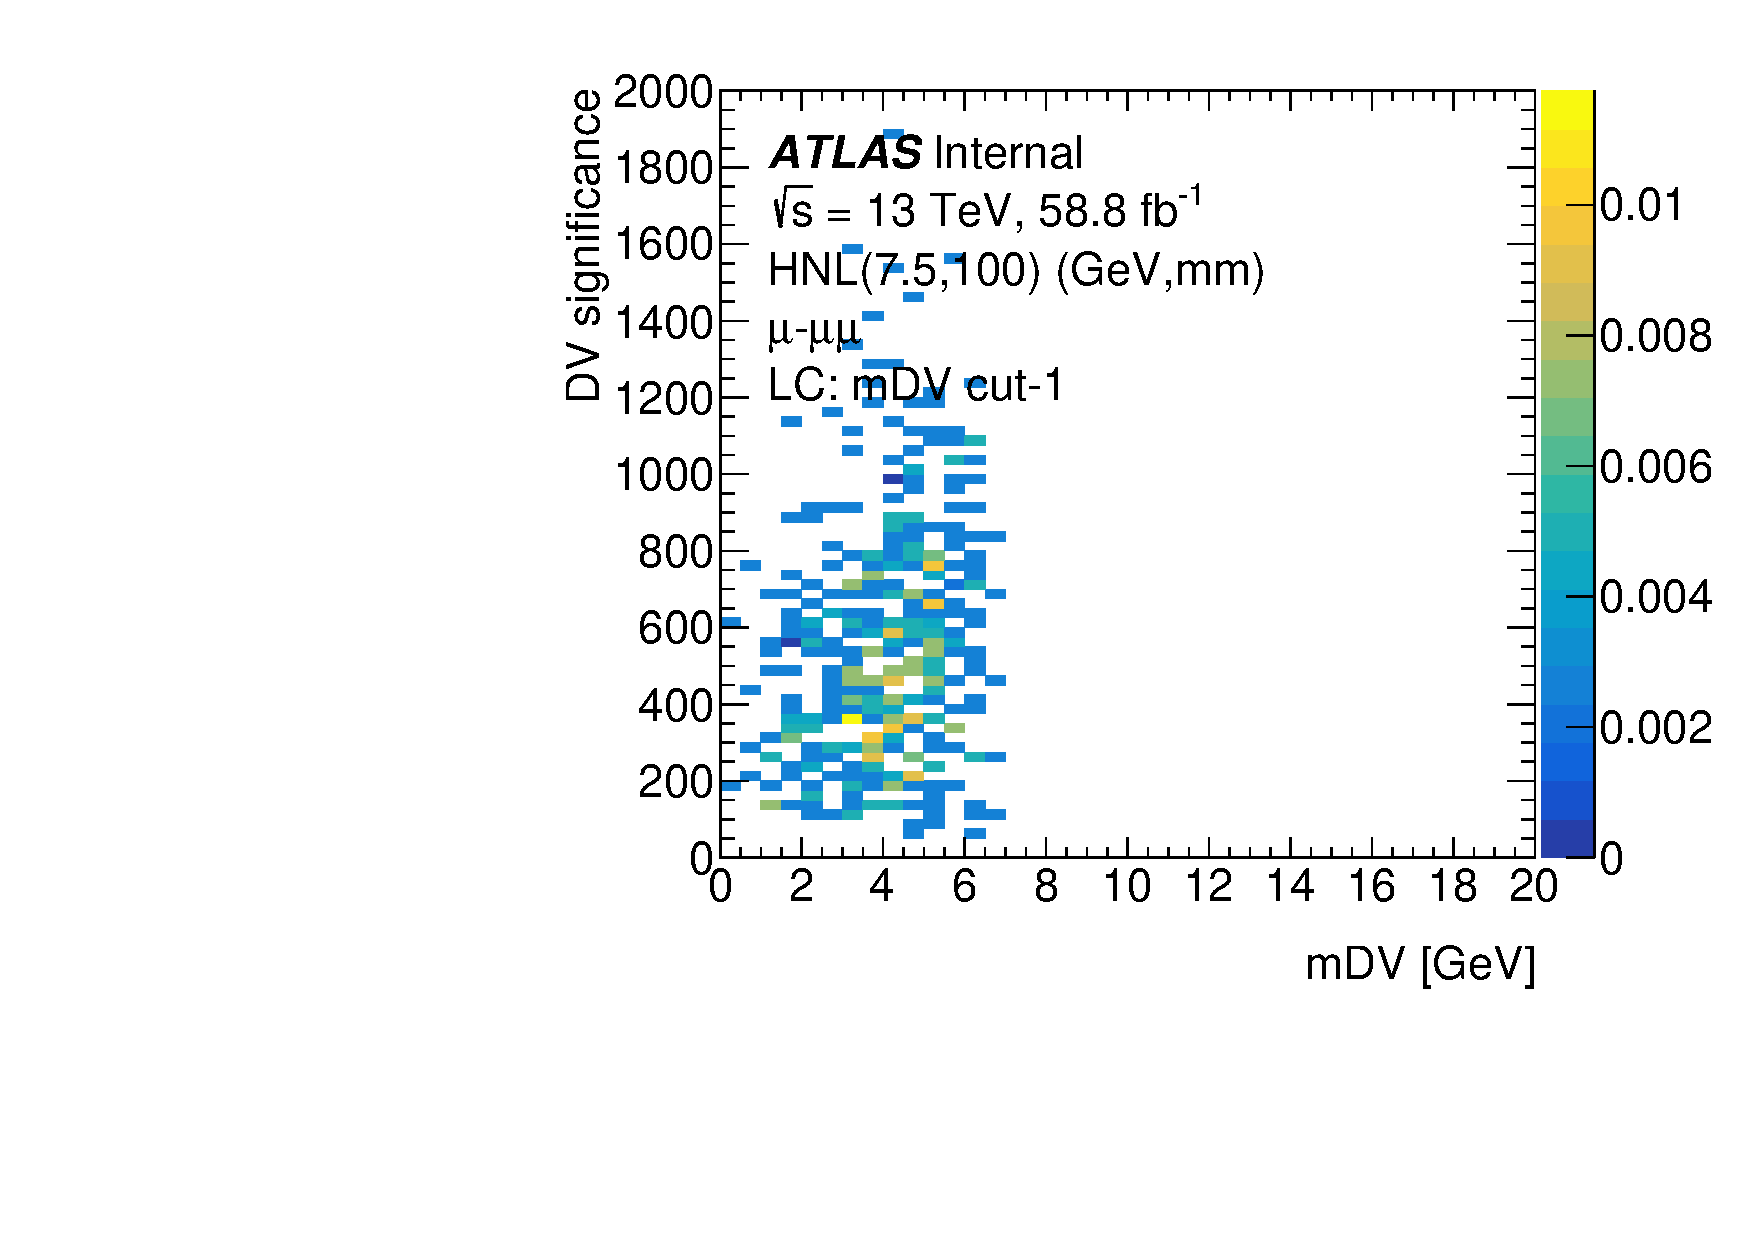
\includegraphics[width=0.45\textwidth]{figures/analysis_strategy/S2D_HNL7p5_ctau100.pdf}}
    \caption{Distribution of events as a function of the $\mathcal{S}$ variable, referred to as `DV significance' in the plots and \mdv.}
    \label{fig:dvsigni_MDV}
\end{figure}

The distribution of events as a function of $\mathcal{S}$ and the mass of the displaced vertex, $m_{\text{DV}}$ is shown in \cref{fig:dvsigni_MDV} for the hadron decay background predicted by the combination of $t\bar{t}$ and $V+$jets MC simulations as well as for representative signals in for pairs (\mhnl, \ctau) = (2 GeV, 1000 mm) and (7.5 GeV, 100 mm).

From~\cref{fig:dvsigni_MDV}, it is clear that the hadron decay backgrounds are characterised by lower values of $\mathcal{S}$, while for the signal samples the discriminant variable peaks at values above 100. Furthermore, the events from the SM processes are present only for displaced vertices masses below 5 GeV, as they are mostly produced in $B$-hadron decay chains. For these reasons, I decided to apply the following selection to all the events in the analysis: $\mathcal{S}>100$ \textit{if} \mdv$<5$~GeV. This means that all the events outside of the rectangle defined by the four coordinates (0,0), (5,0), (0,100), (5,100) in the $(\mdv\,[\text{GeV}],\mathcal{S})$ plane are retained.

The SR is defined by requiring, on top of the events pre-selection, that the two displaced leptons satisfy an isolation criterion, using the \texttt{Loose\_VarRad}~\cite{EGAM-2018-01} WP for electrons, and the \texttt{PflowLoose\_VarRad} WP~\cite{MUON-2018-03} for muons. Leptons from the DV tend to be collimated and hence close-by-effects\footnote{The calculation of isolation variables uses low-level information from the tracker and the calorimeter without relying on object-level reconstruction. When two leptons are close to each other, they will contribute to the calculation of each other's isolation variables. However, since isolation is only supposed to identify leptons in jets, such a lepton-close-by-effect is an artefact of the method and needs to be corrected.} that might appear in the evaluation of isolation variables are taken into account and correctly subtracted from both the track term and the calorimeter term that define the isolation working points. This procedure is done since Run-1 in $H\to ZZ^*\to 4\ell$ analyses, and generally applies to boosted multi-lepton signatures utilizing lepton isolation. The HF-CR, on the other hand, is defined adding a requirement of at least one non-isolated displaced lepton. To further suppress signal contamination in this region, at least one b-tagged jet is required. This requirement does not bias the kinematics of the correlated background in the HF-CR away from the SR. Lastly, since this analysis probes HNLs with masses up to 20 GeV, the phase space beyond \mhnl$>20$~GeV is not considered in the SR. ~\Cref{tab:sr_cr_cuts} summarizes the cuts used for the SR and the HF-CR. There are 6 SRs and 6 HF-CRs defined in this analysis, one each per channel.

\begin{table}[!htbp]
    \centering
    \resizebox{\columnwidth}{!}{
    \begin{tabular}{>{\centering}p{0.4\textwidth-70pt}
                    >{\centering}p{0.3\textwidth}
                    cp{0.3\textwidth-220pt}}
         \hline\hline
         Cut Name &  \multicolumn{2}{c}{Cut Description} \\
         \hline
         \multicolumn{3}{c}{\textbf{Object Selection}} \\
         \hline
         Primary Vertex &  \multicolumn{2}{c}{Largest $\Sigma_\mathrm{tracks} \pT^2$} \\
         Prompt Lepton &  \multicolumn{2}{c}{see~\cref{tab:plep_selection}} \\
         Trigger & \multicolumn{2}{c}{see~\cref{tab:triggers}} \\
         Displaced Lepton &  \multicolumn{2}{c}{see~\cref{tab:disp_muon_selection,tab:disp_electron_selection}} \\
         Overlap Removal &  \multicolumn{2}{c}{see~\cref{tab:overlap_removal}} \\
         Displaced Vertex &  \multicolumn{2}{c}{see~\cref{tab:dv_selection}} \\
         \hline
         \multicolumn{3}{c}{\textbf{Pre-selection}} \\
         \hline
         $\gamma\to e e$ Veto & \multicolumn{2}{c}{Material veto, $|z|<300$~mm and $\mdv>500$~MeV for $ee$ DVs} \\
         Cosmic Muon Veto & \multicolumn{2}{c}{$\sqrt{(\Sigma_\text{DV tracks}\eta)^2+(\pi-|\Delta_\text{DV tracks}\phi|)^2}>.05$}\\
         $Z\to\ell\ell$ Veto & \multicolumn{2}{c}{$|m_{\ell_\mathrm{DV}\ell_\mathrm{prompt}}-90\text{ GeV}|>10\text{ GeV}$ for SFOS pairs} \\
         $W$-decay Selection & \multicolumn{2}{c}{40 GeV $<m_{\ell\ell\ell}<90$ GeV} \\
         $J/\psi$ Veto & \multicolumn{2}{c}{$|\mdv-3.1\text{ GeV}|>0.1\text{ GeV}$ for $ee$ and $\mu\mu$ DVs} \\
         Discriminant & \multicolumn{2}{c}{$\mathcal{S}>100$ \textit{if} \mdv$<5$~GeV} \\
         \hline
         \multicolumn{3}{c}{\textbf{Region Specific Cuts}} \\
         \hline
         & \textbf{SR} & \textbf{HF-CR} \\
         \hline
         DV Lepton Isolation & Both isolated & $\geq 1$ non-isolated \\
         b-jets & - & $\geq 1$ \\
         \mhnl Limit & $<20$~GeV & - \\
         \hline\hline
    \end{tabular}
    }
    \caption{Object selection, pre-selection, and other additional cuts used to define the non-overlapping Signal Region and the Heavy Flavor Control Region.}
    \label{tab:sr_cr_cuts}
\end{table}

~\Cref{fig:cr_plots_uuu,fig:cr_plots_uue,fig:cr_plots_uee,fig:cr_plots_euu,fig:cr_plots_eeu,fig:cr_plots_eee} show representative kinematics of important properties of the DV in the event and the tracks in it, the prompt lepton, and the $\mathcal{S}$ discriminant variable for events in the HF-CR for all the six channels.

\begin{figure}[!ht]
    \centering
    \subfloat[{\mdv [GeV]}]{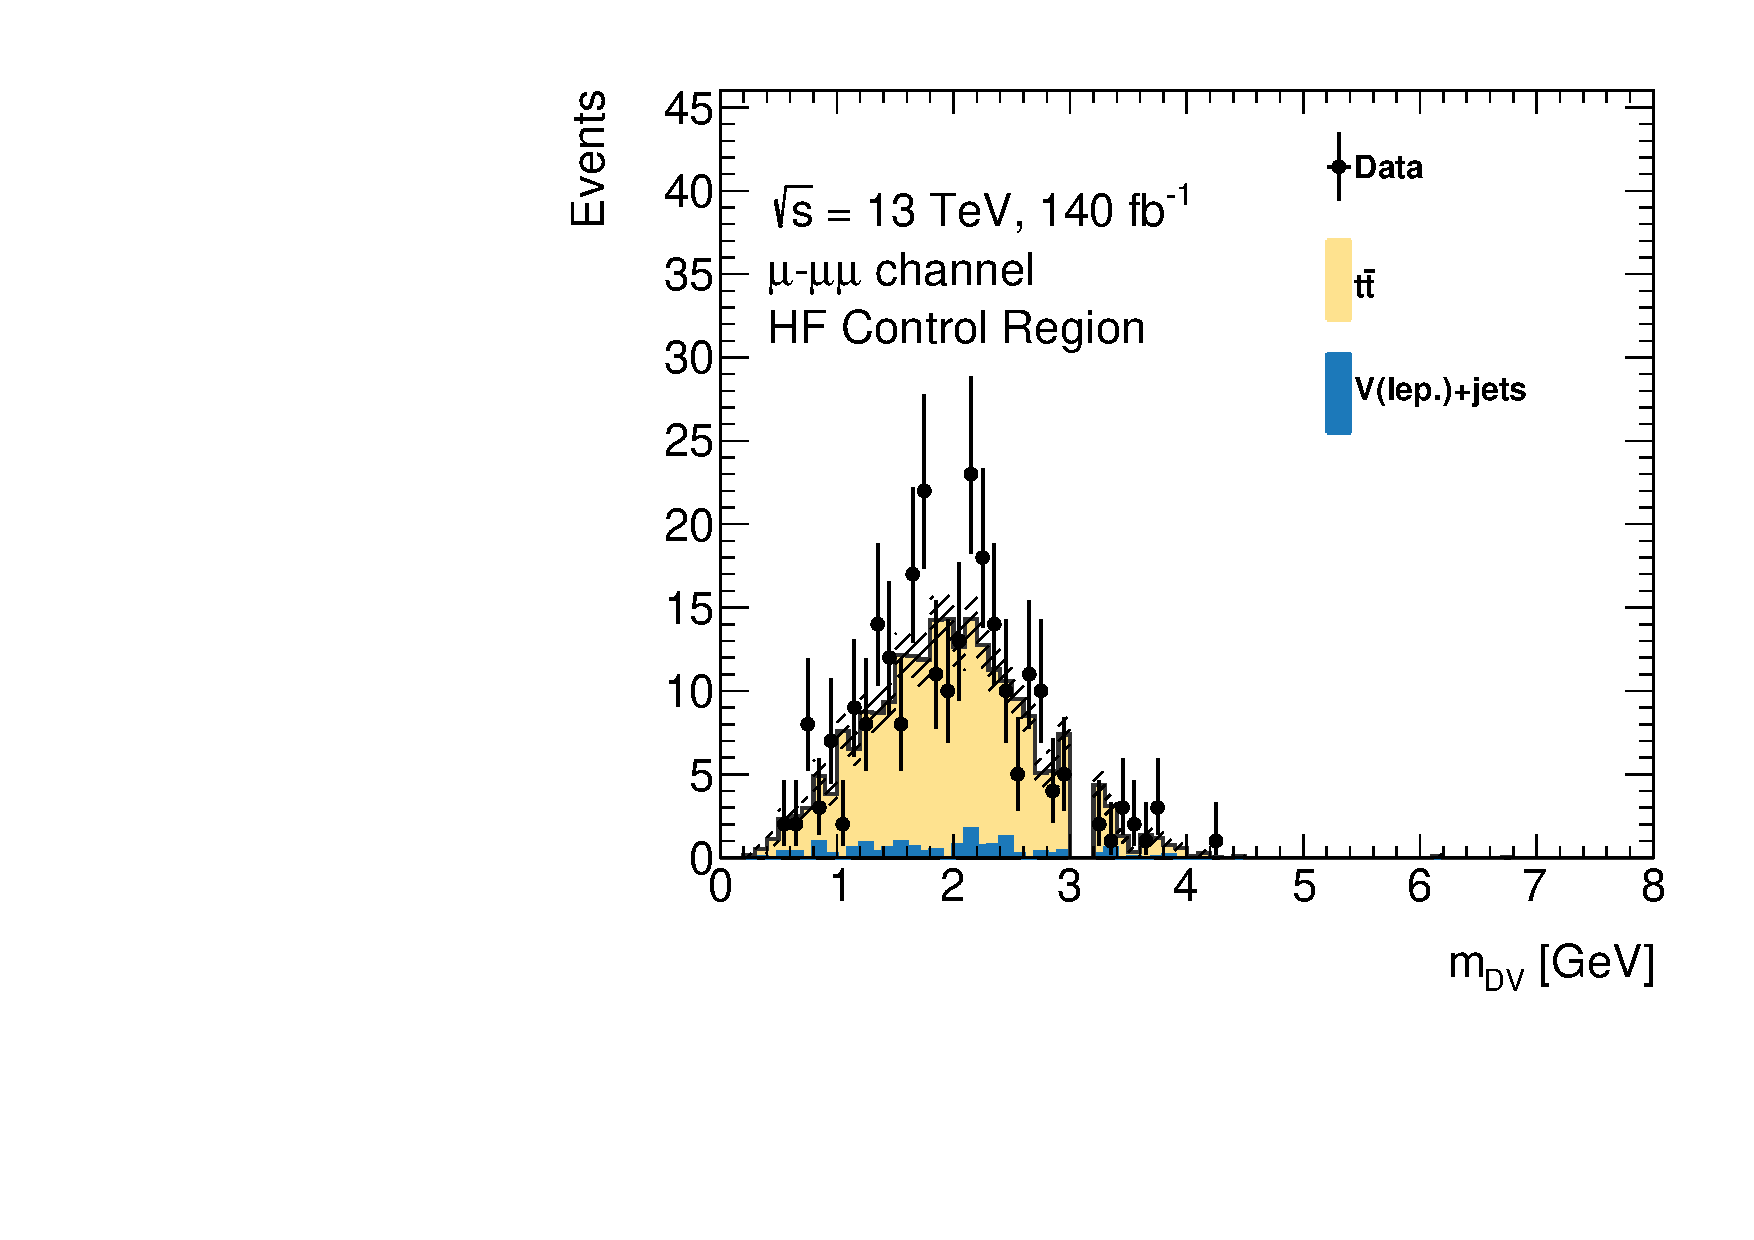
\includegraphics[width=0.24\linewidth]{figures/analysis_strategy/CR_plots/uuu/DV_mass.pdf}}
    \subfloat[{$r_\mathrm{DV}$ [mm]}]{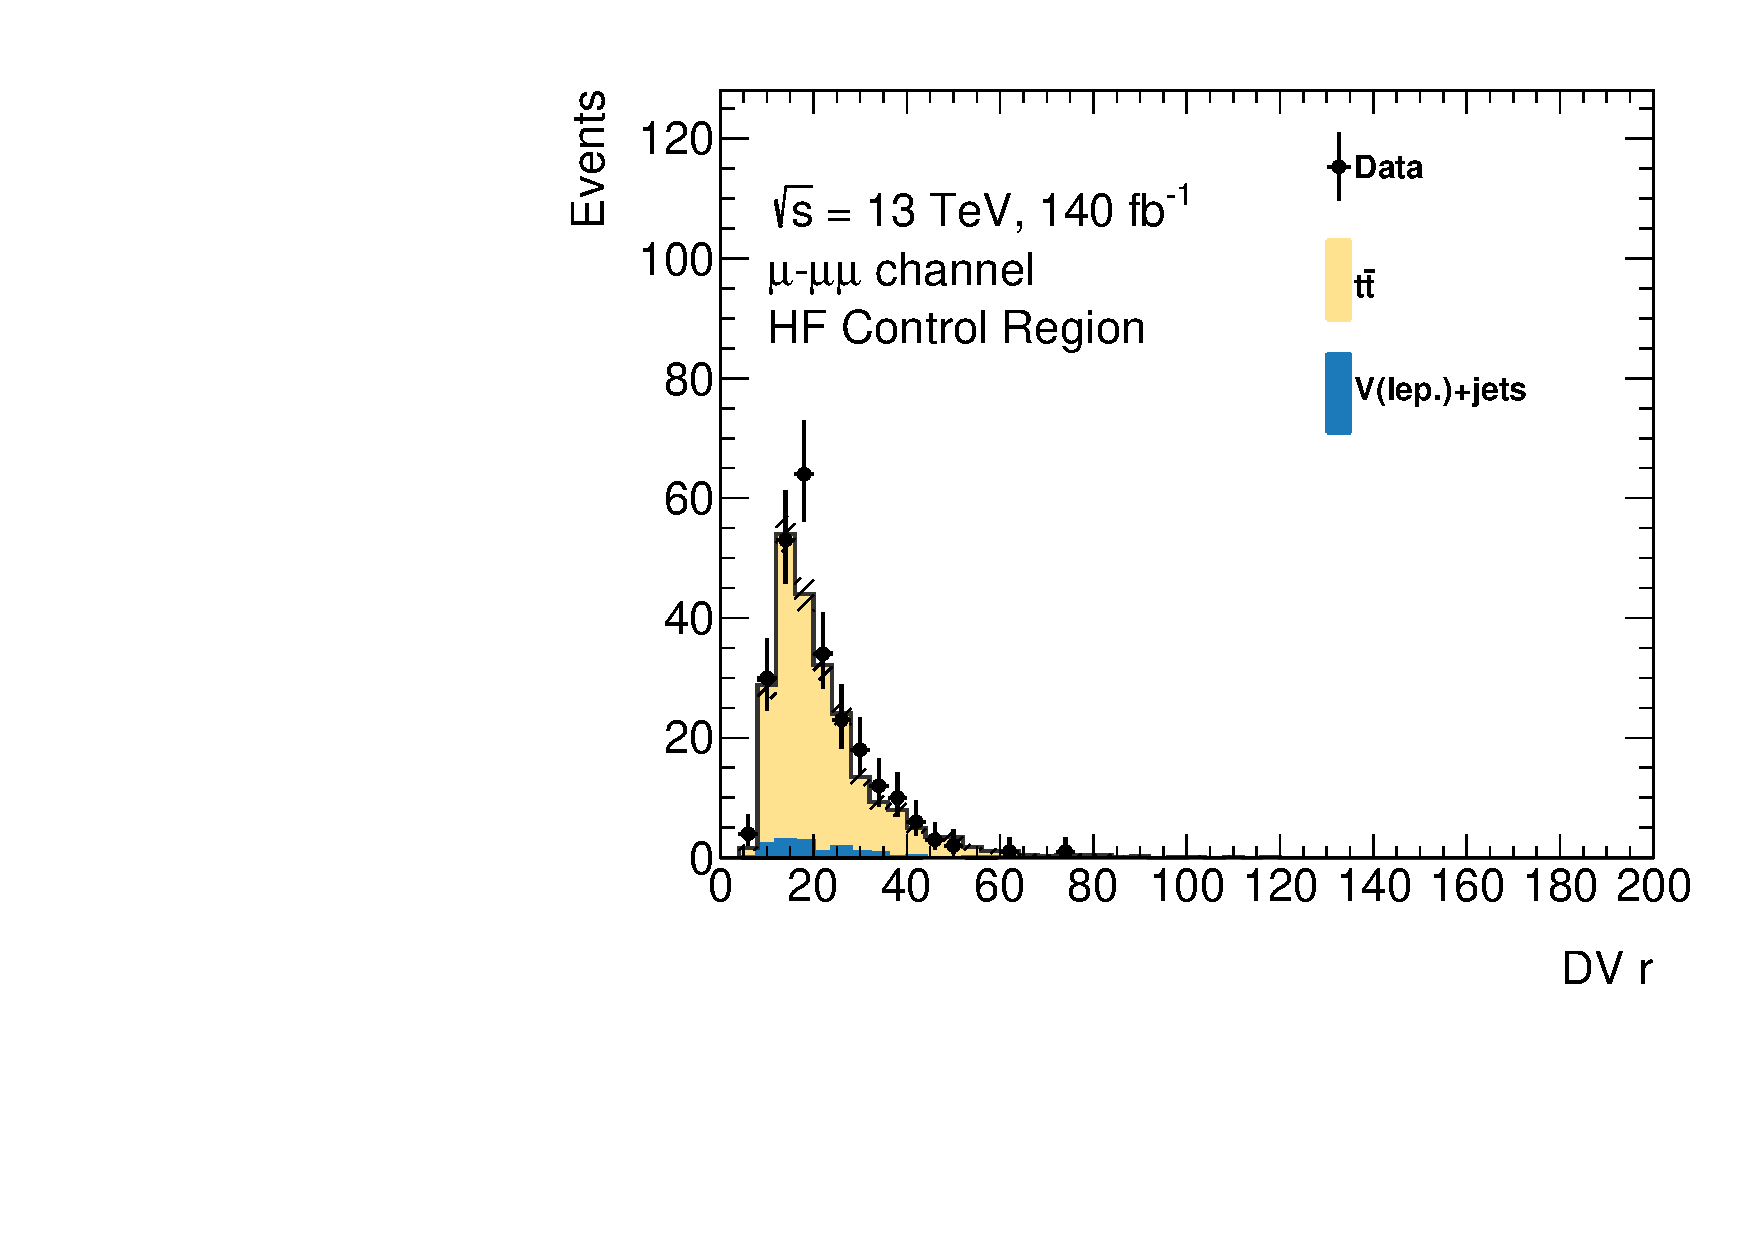
\includegraphics[width=0.24\linewidth]{figures/analysis_strategy/CR_plots/uuu/DV_r.pdf}}
    \subfloat[{$\mathcal{S}$}]{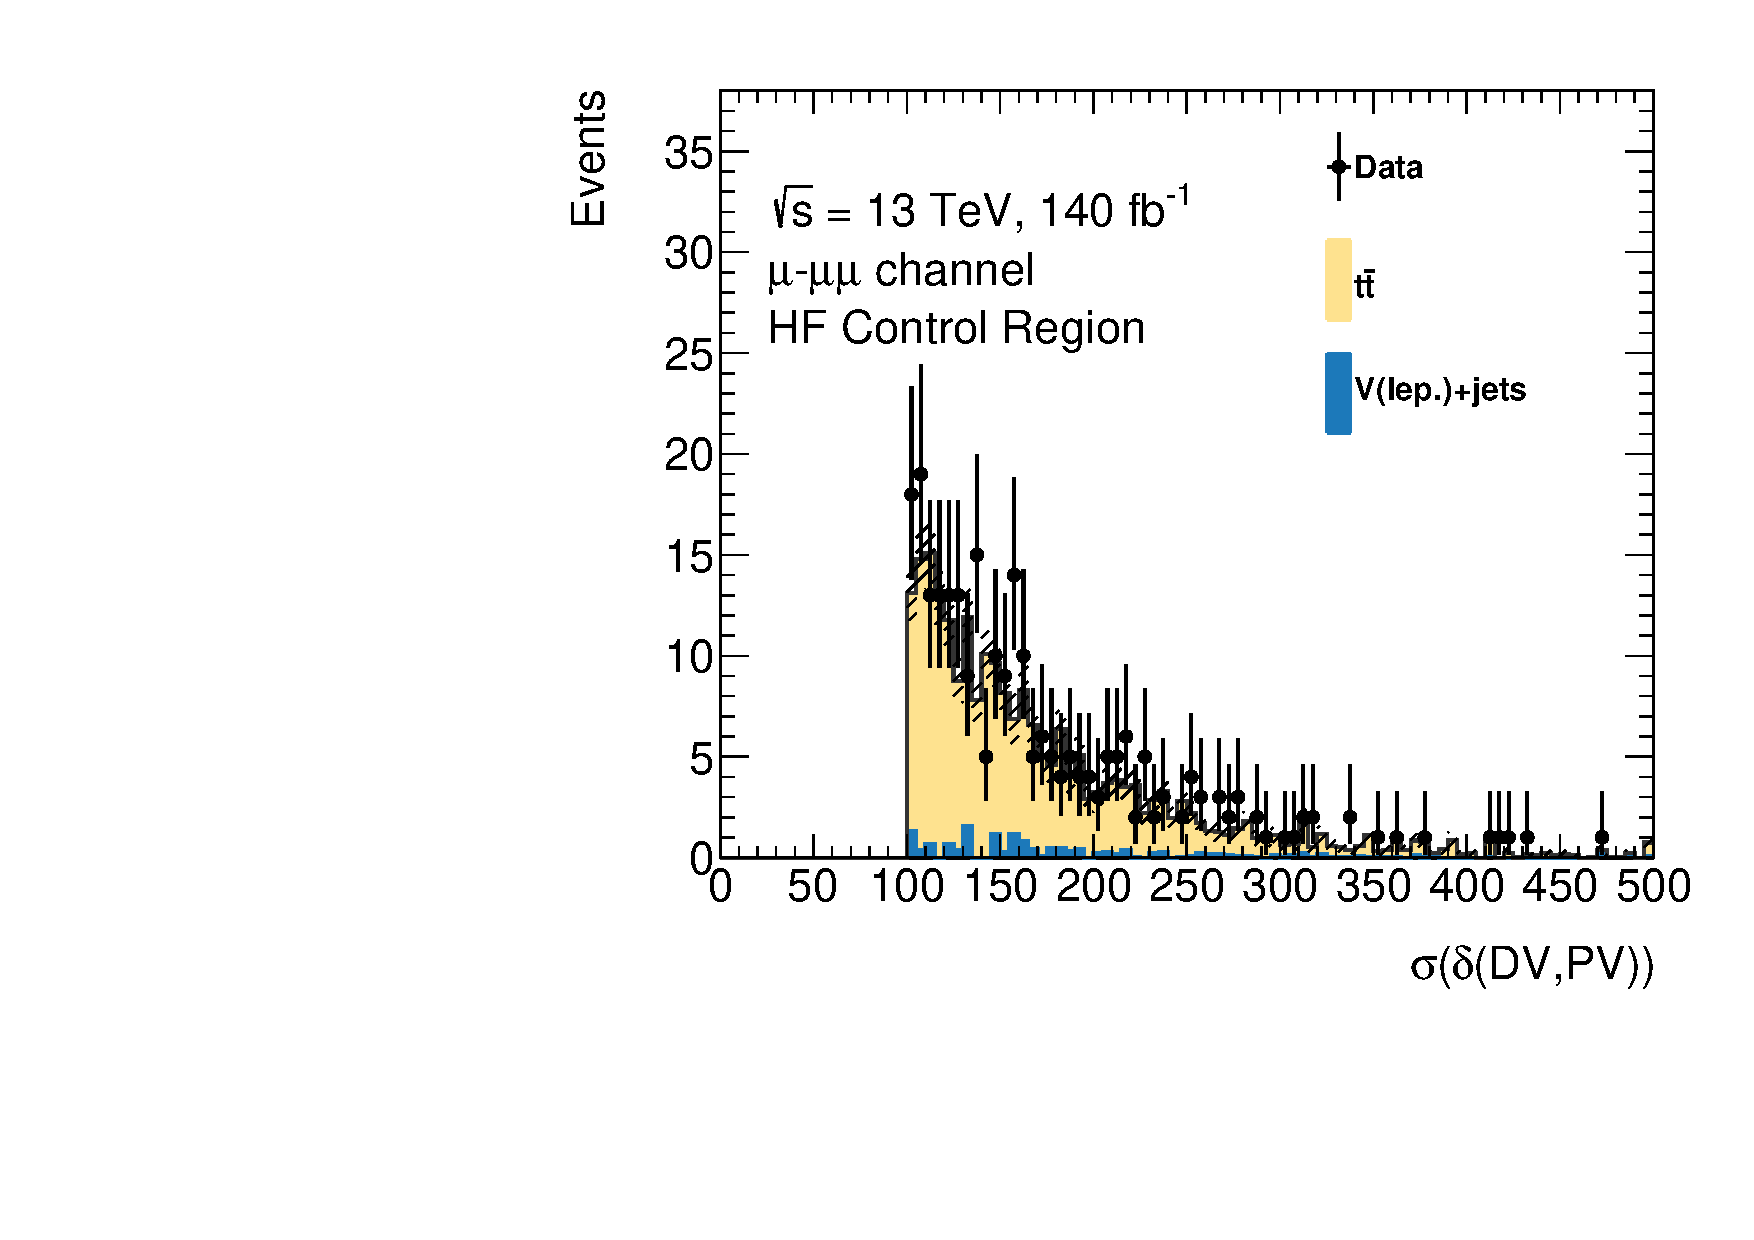
\includegraphics[width=0.24\linewidth]{figures/analysis_strategy/CR_plots/uuu/DV_distFromPVsigni.pdf}}
    \subfloat[{prompt lep. \pT [GeV]}]{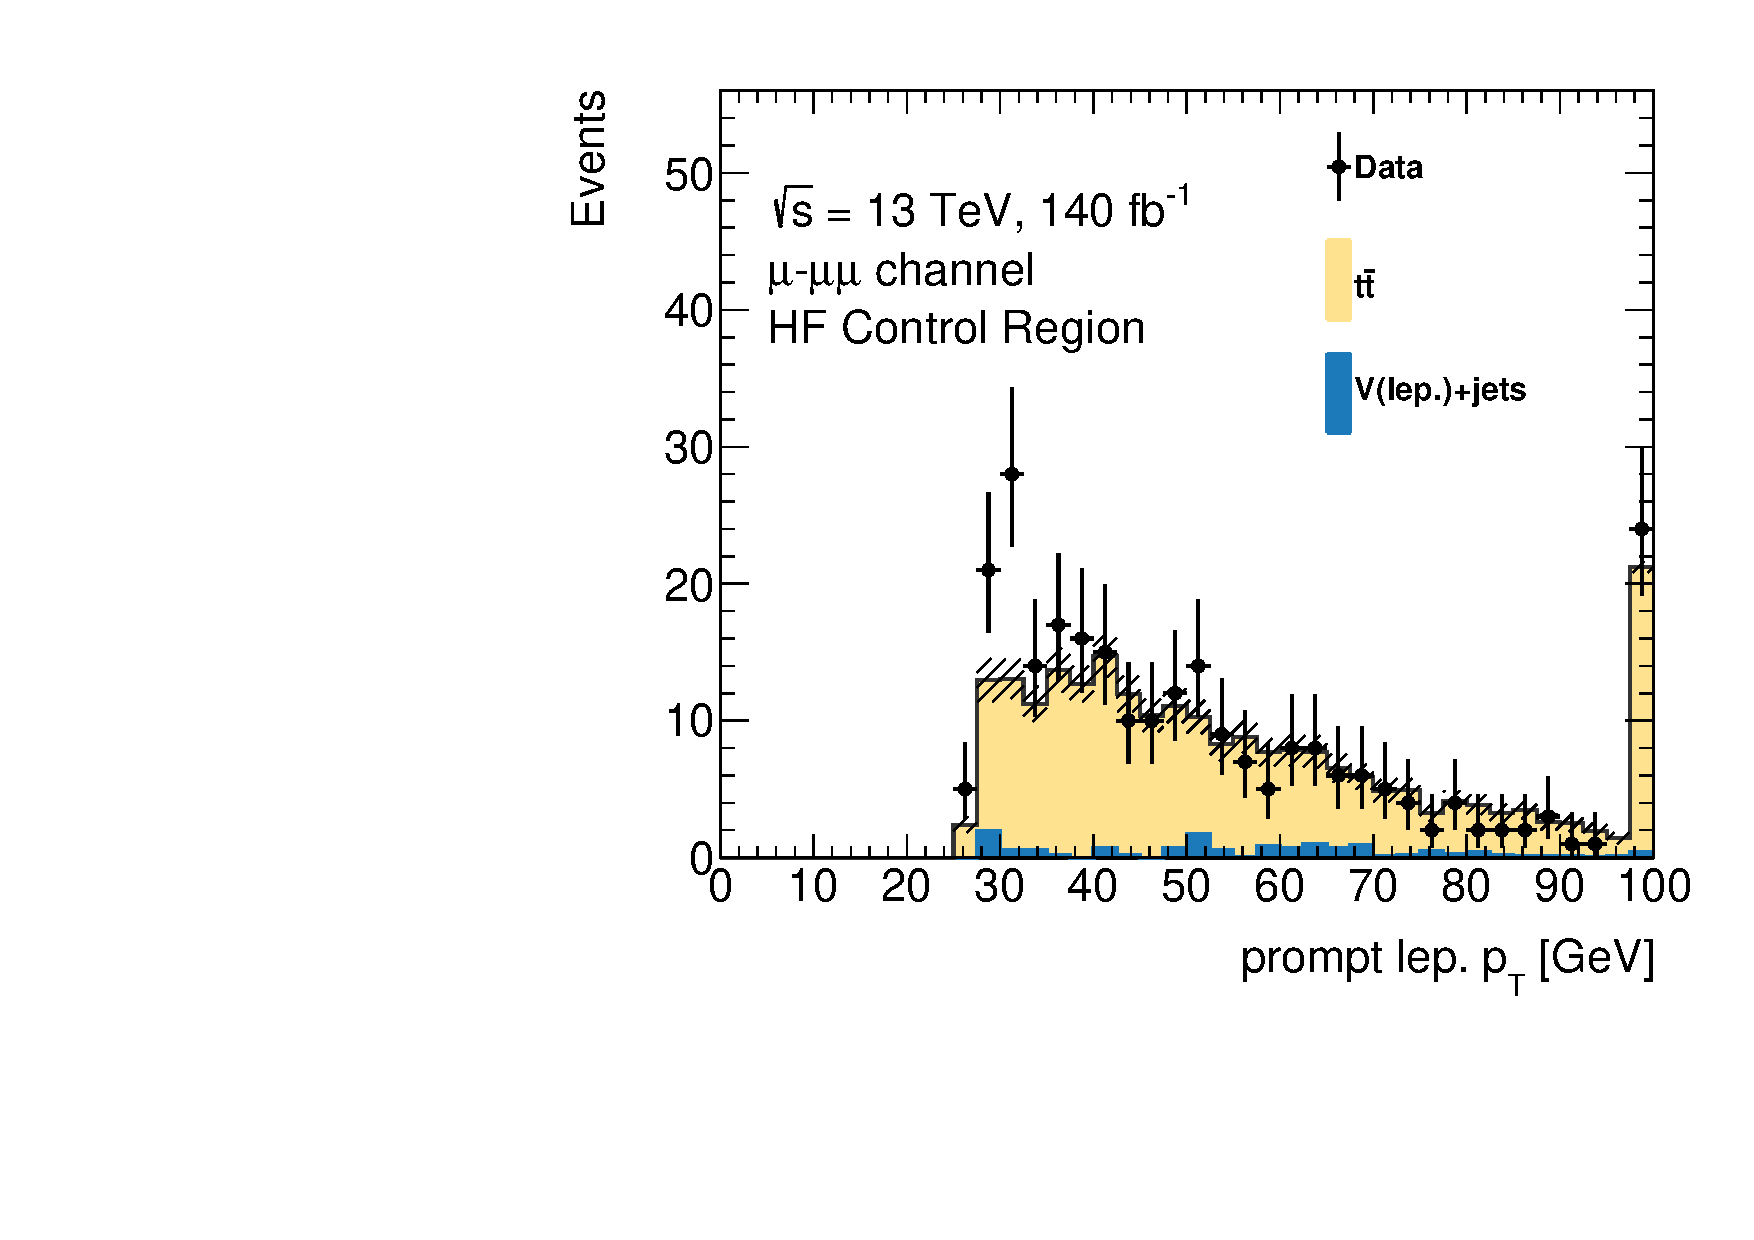
\includegraphics[width=0.24\linewidth]{figures/analysis_strategy/CR_plots/uuu/prompt_lepton_pt.pdf}}\\
    \subfloat[{$\Delta R$ DV tracks}]{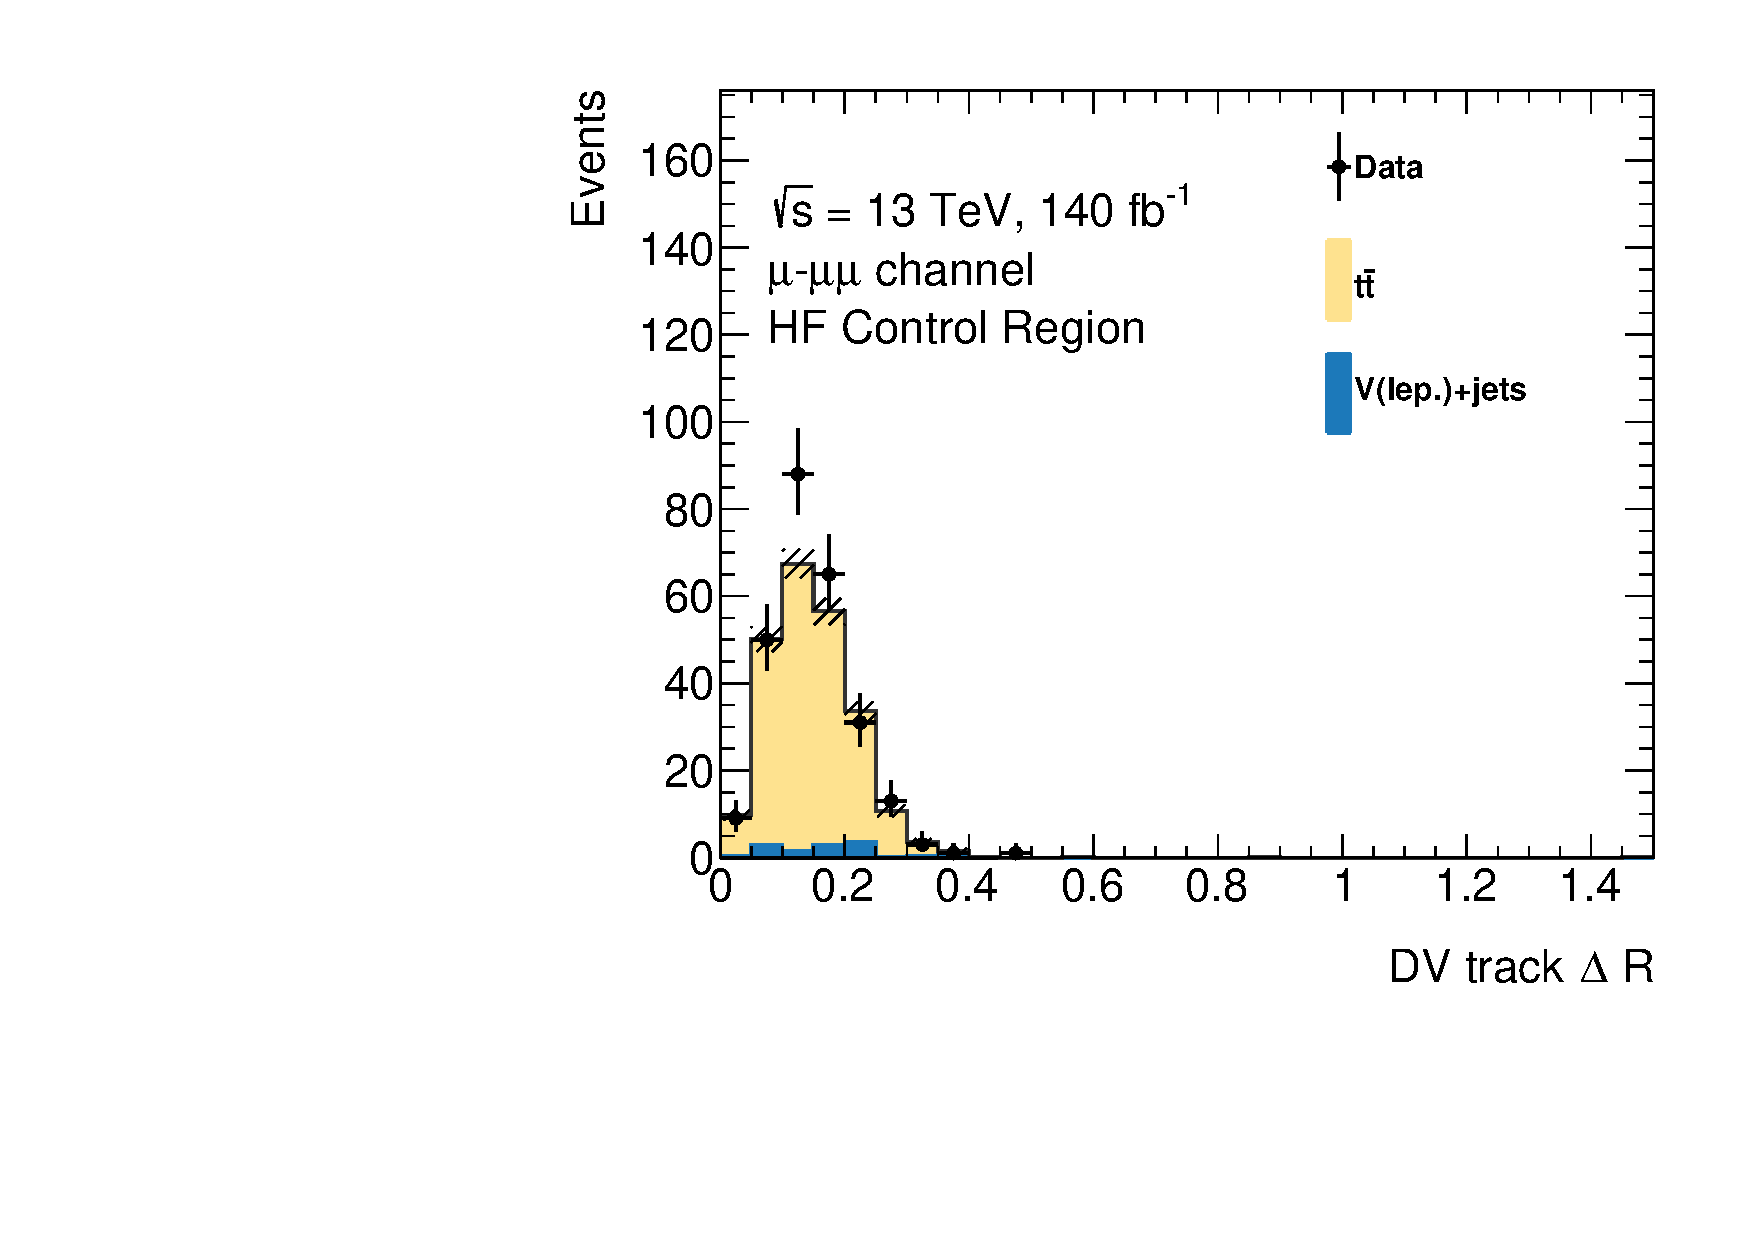
\includegraphics[width=0.24\linewidth]{figures/analysis_strategy/CR_plots/uuu/DV_track_dR.pdf}}
    \subfloat[{\pT of DV tracks [GeV]}]{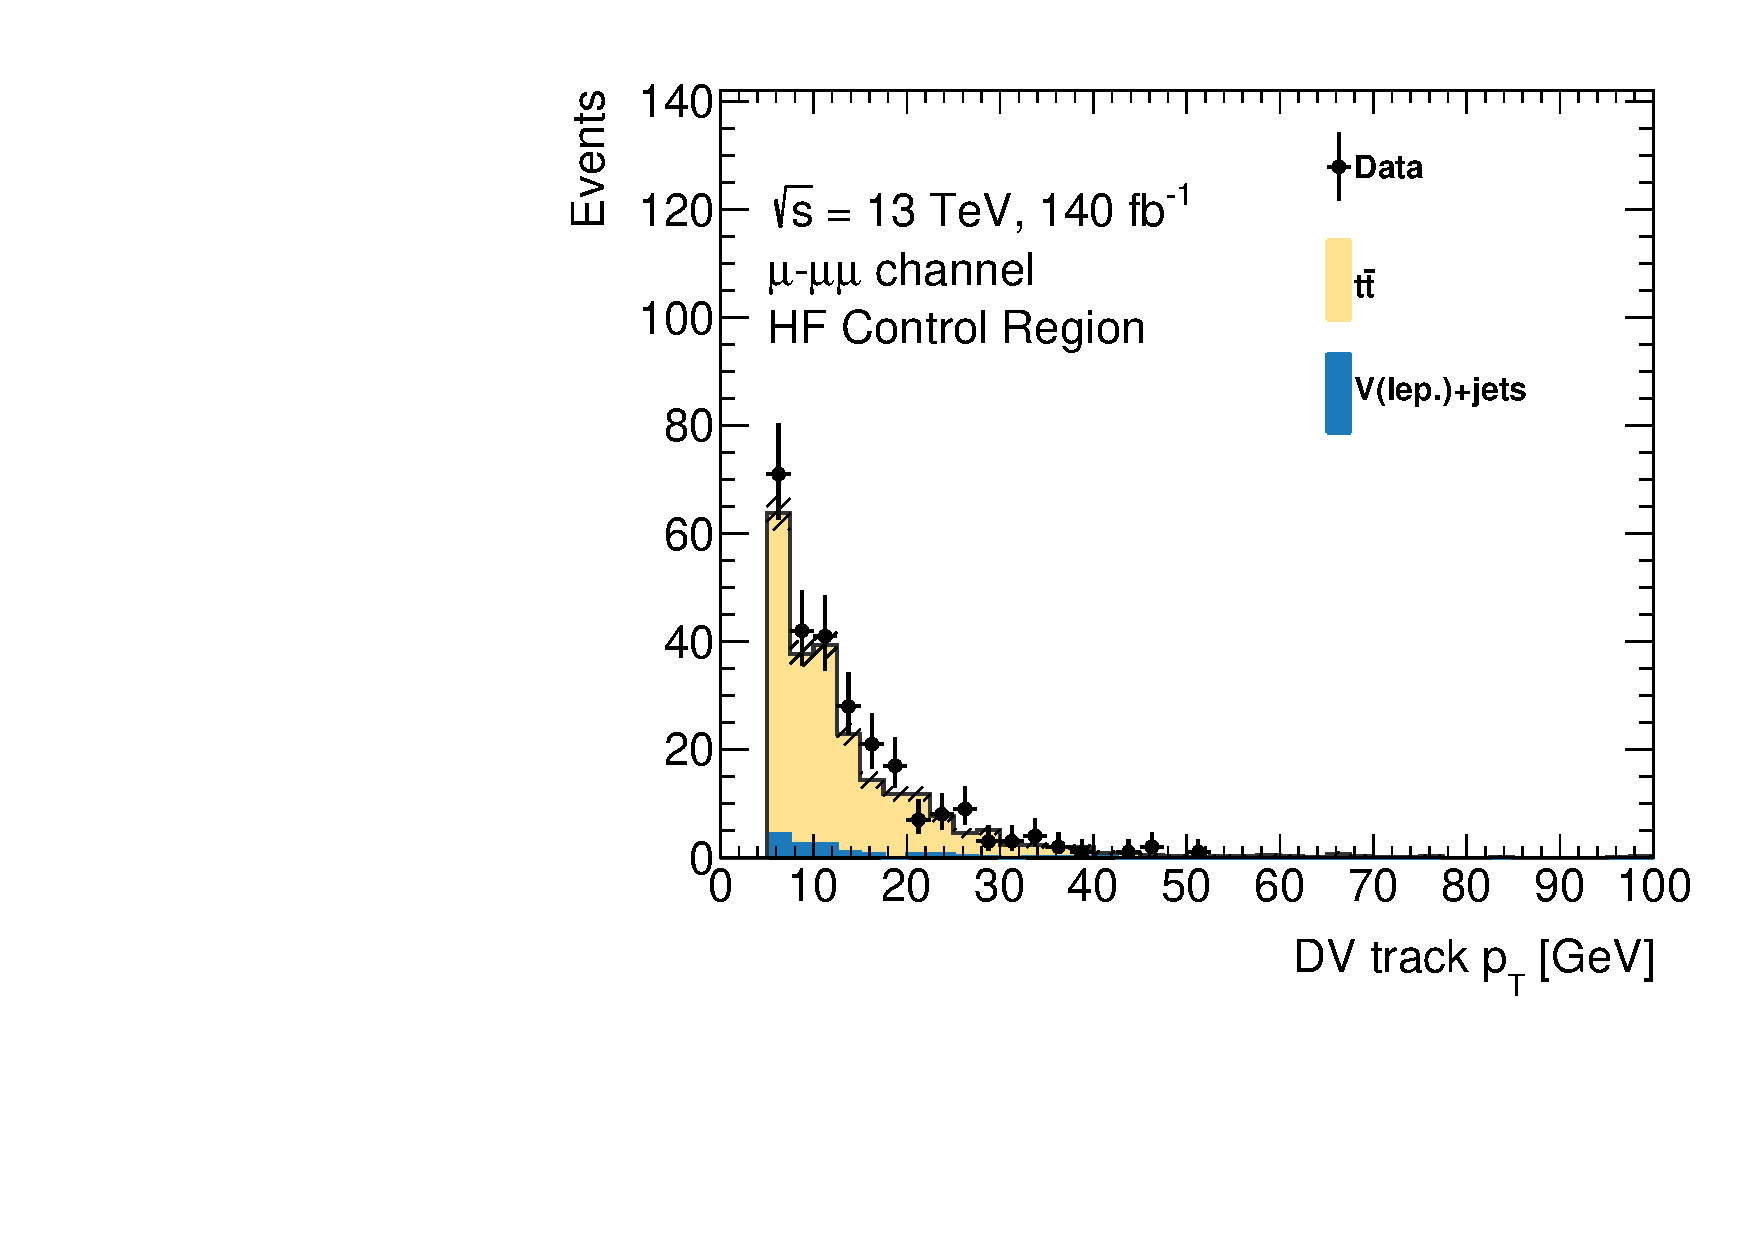
\includegraphics[width=0.24\linewidth]{figures/analysis_strategy/CR_plots/uuu/DV_trk_pt.pdf}}
    \subfloat[{$\eta$ of DV tracks}]{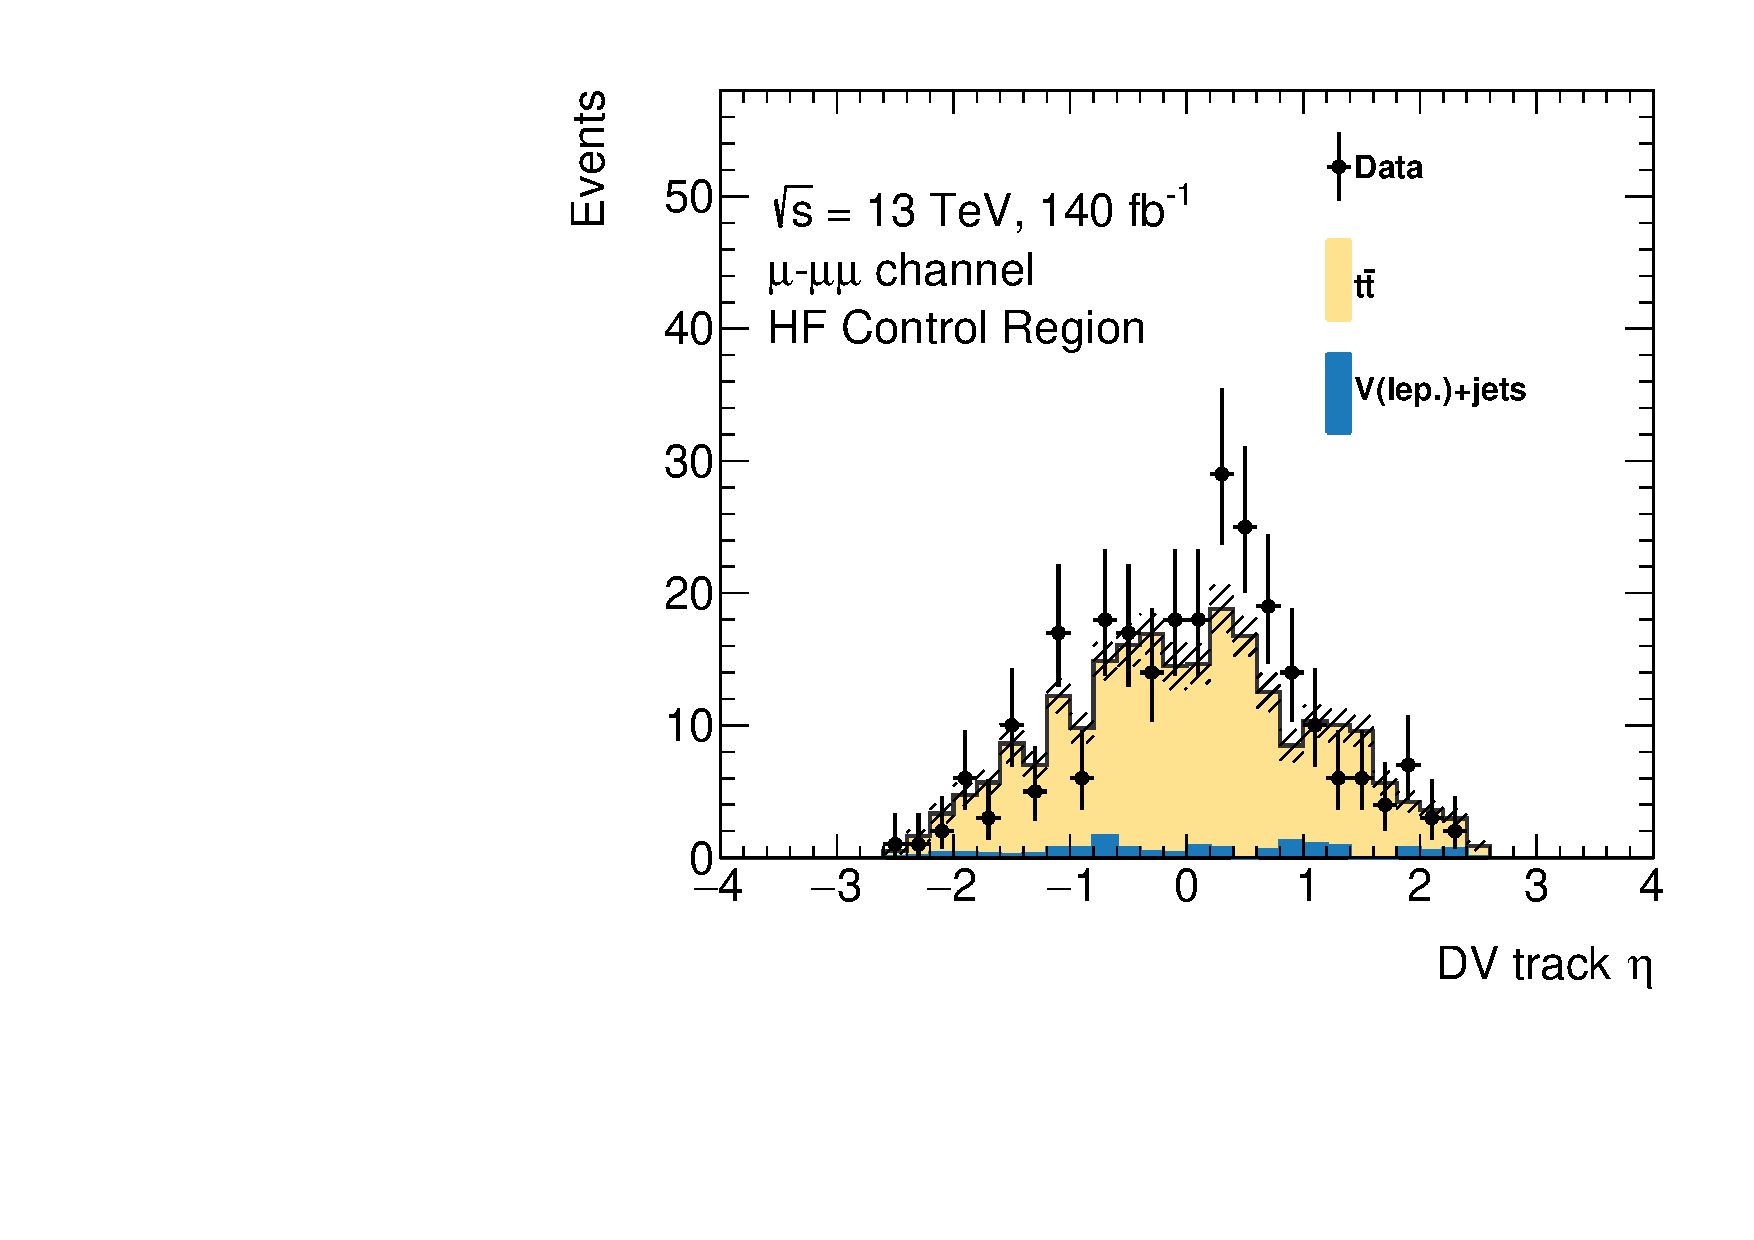
\includegraphics[width=0.24\linewidth]{figures/analysis_strategy/CR_plots/uuu/DV_trk_eta.pdf}}
    \subfloat[{$d_0$ of DV tracks [mm]}]{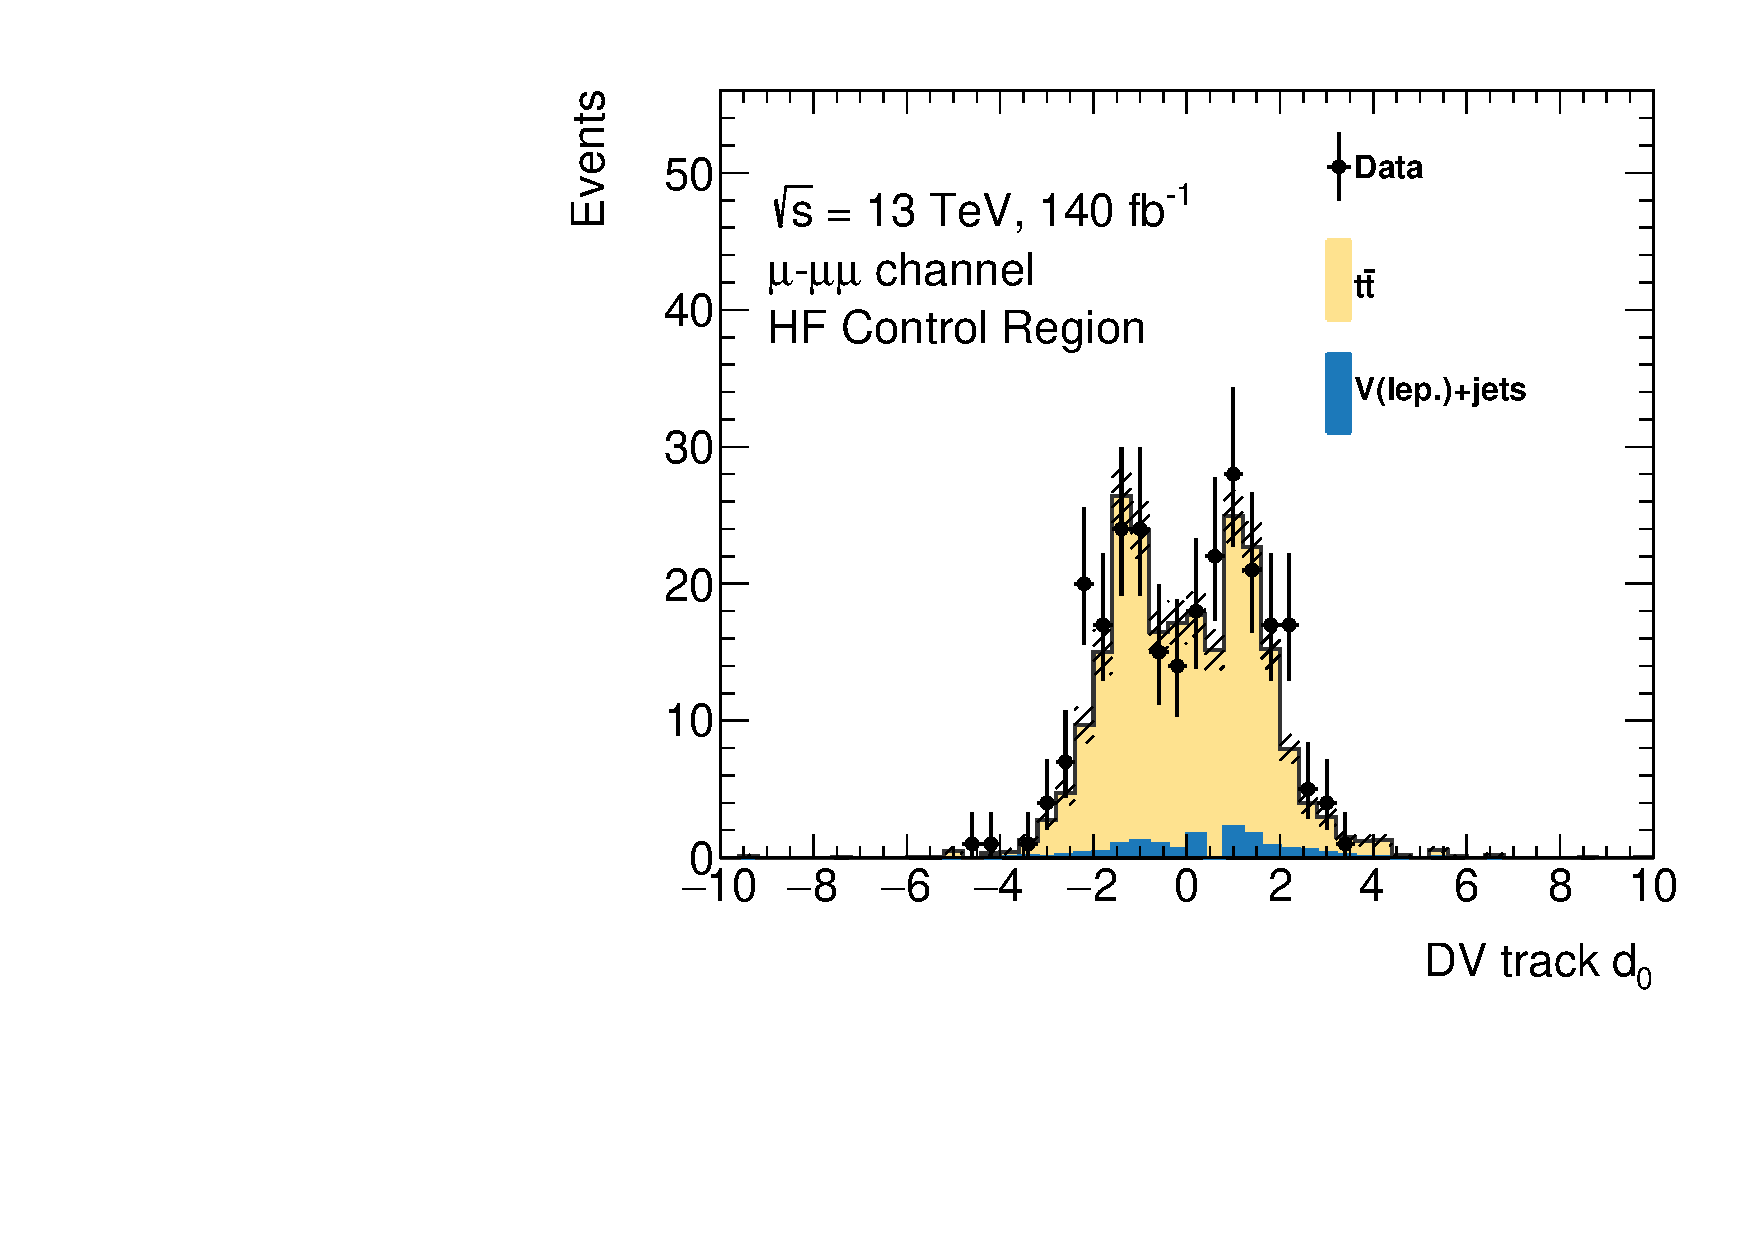
\includegraphics[width=0.24\linewidth]{figures/analysis_strategy/CR_plots/uuu/DV_trk_d0.pdf}}
    \caption{Representative kinematics of the displaced vertex, tracks in the displaced vertex, and of the prompt lepton measured in ATLAS data and modeled by MC simulations in the \uuu Heavy Flavor Control Region.}
    \label{fig:cr_plots_uuu}
\end{figure}

\begin{figure}[!ht]
    \centering
    \subfloat[{\mdv [GeV]}]{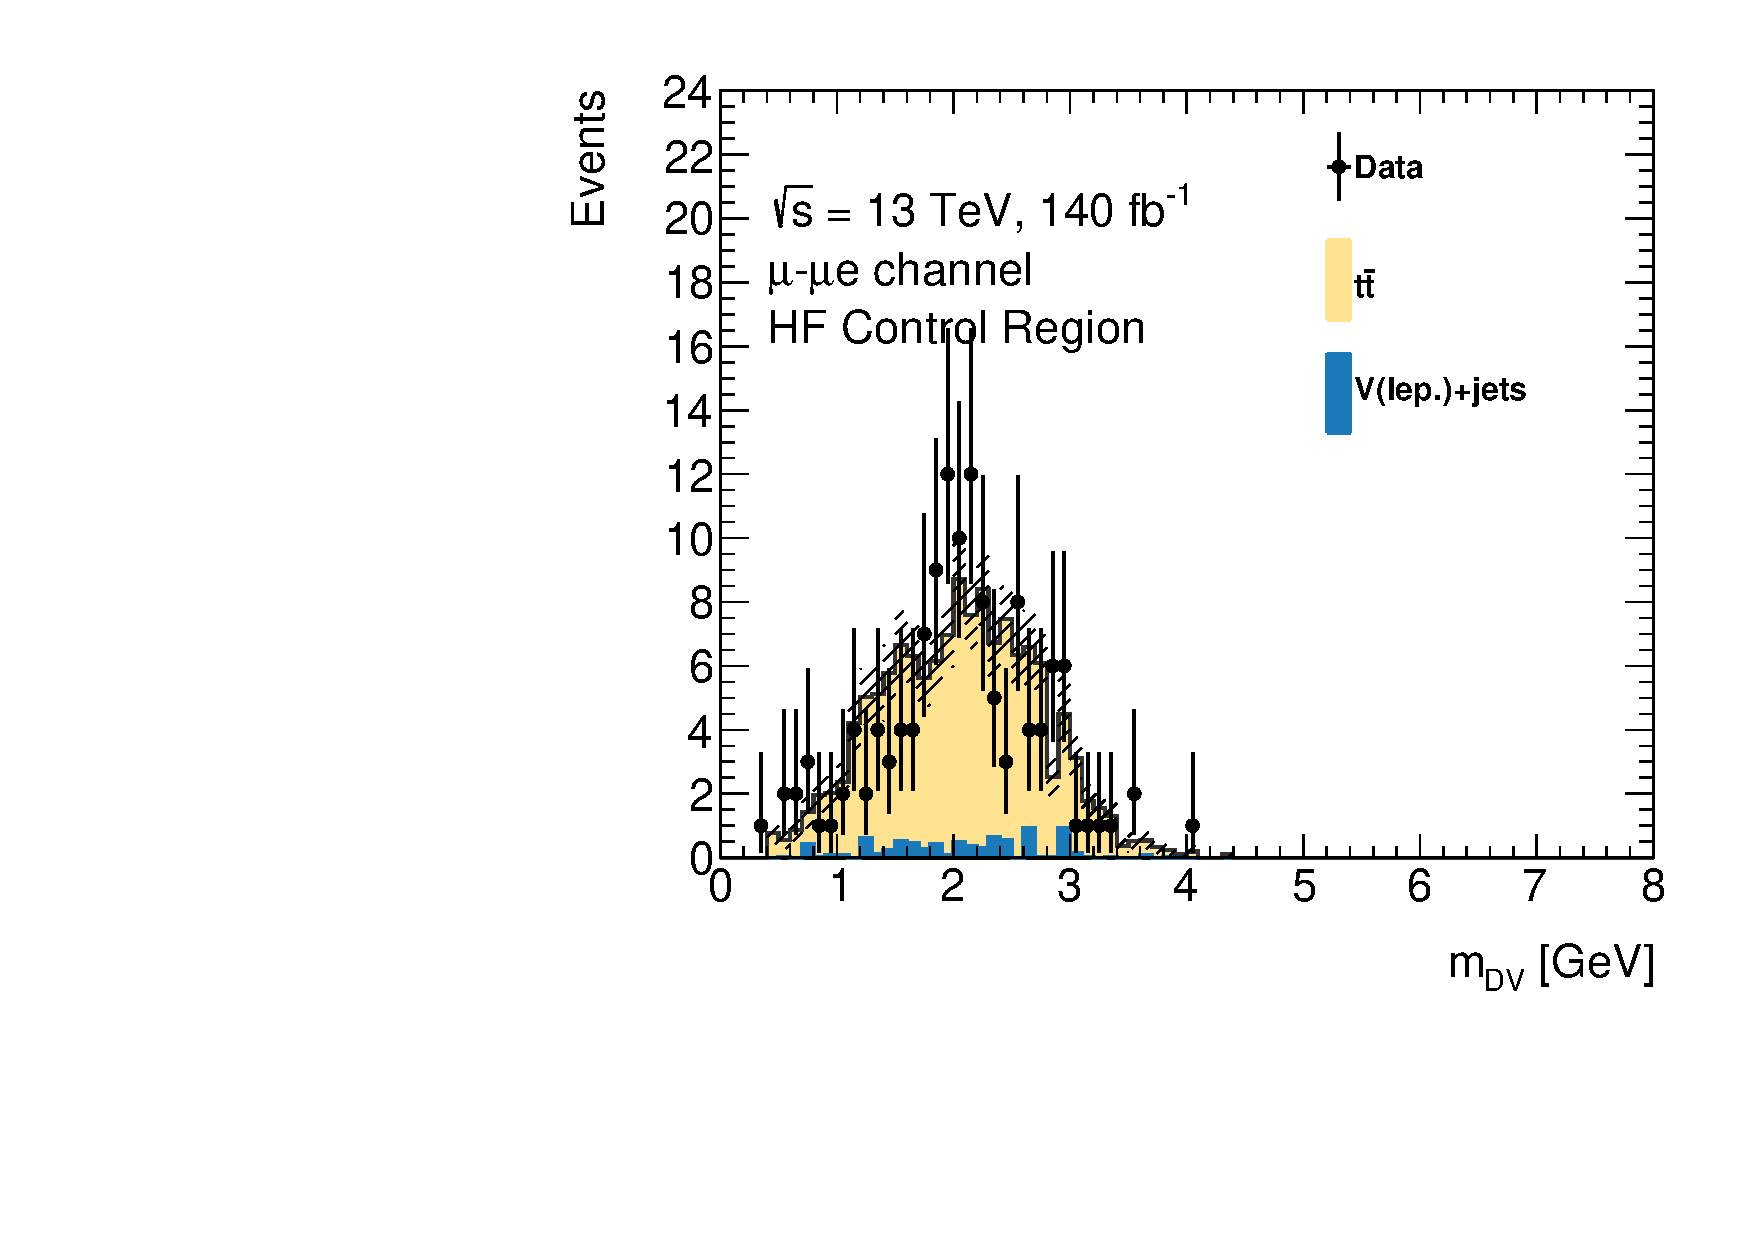
\includegraphics[width=0.24\linewidth]{figures/analysis_strategy/CR_plots/uue/DV_mass.pdf}}
    \subfloat[{$r_\mathrm{DV}$ [mm]}]{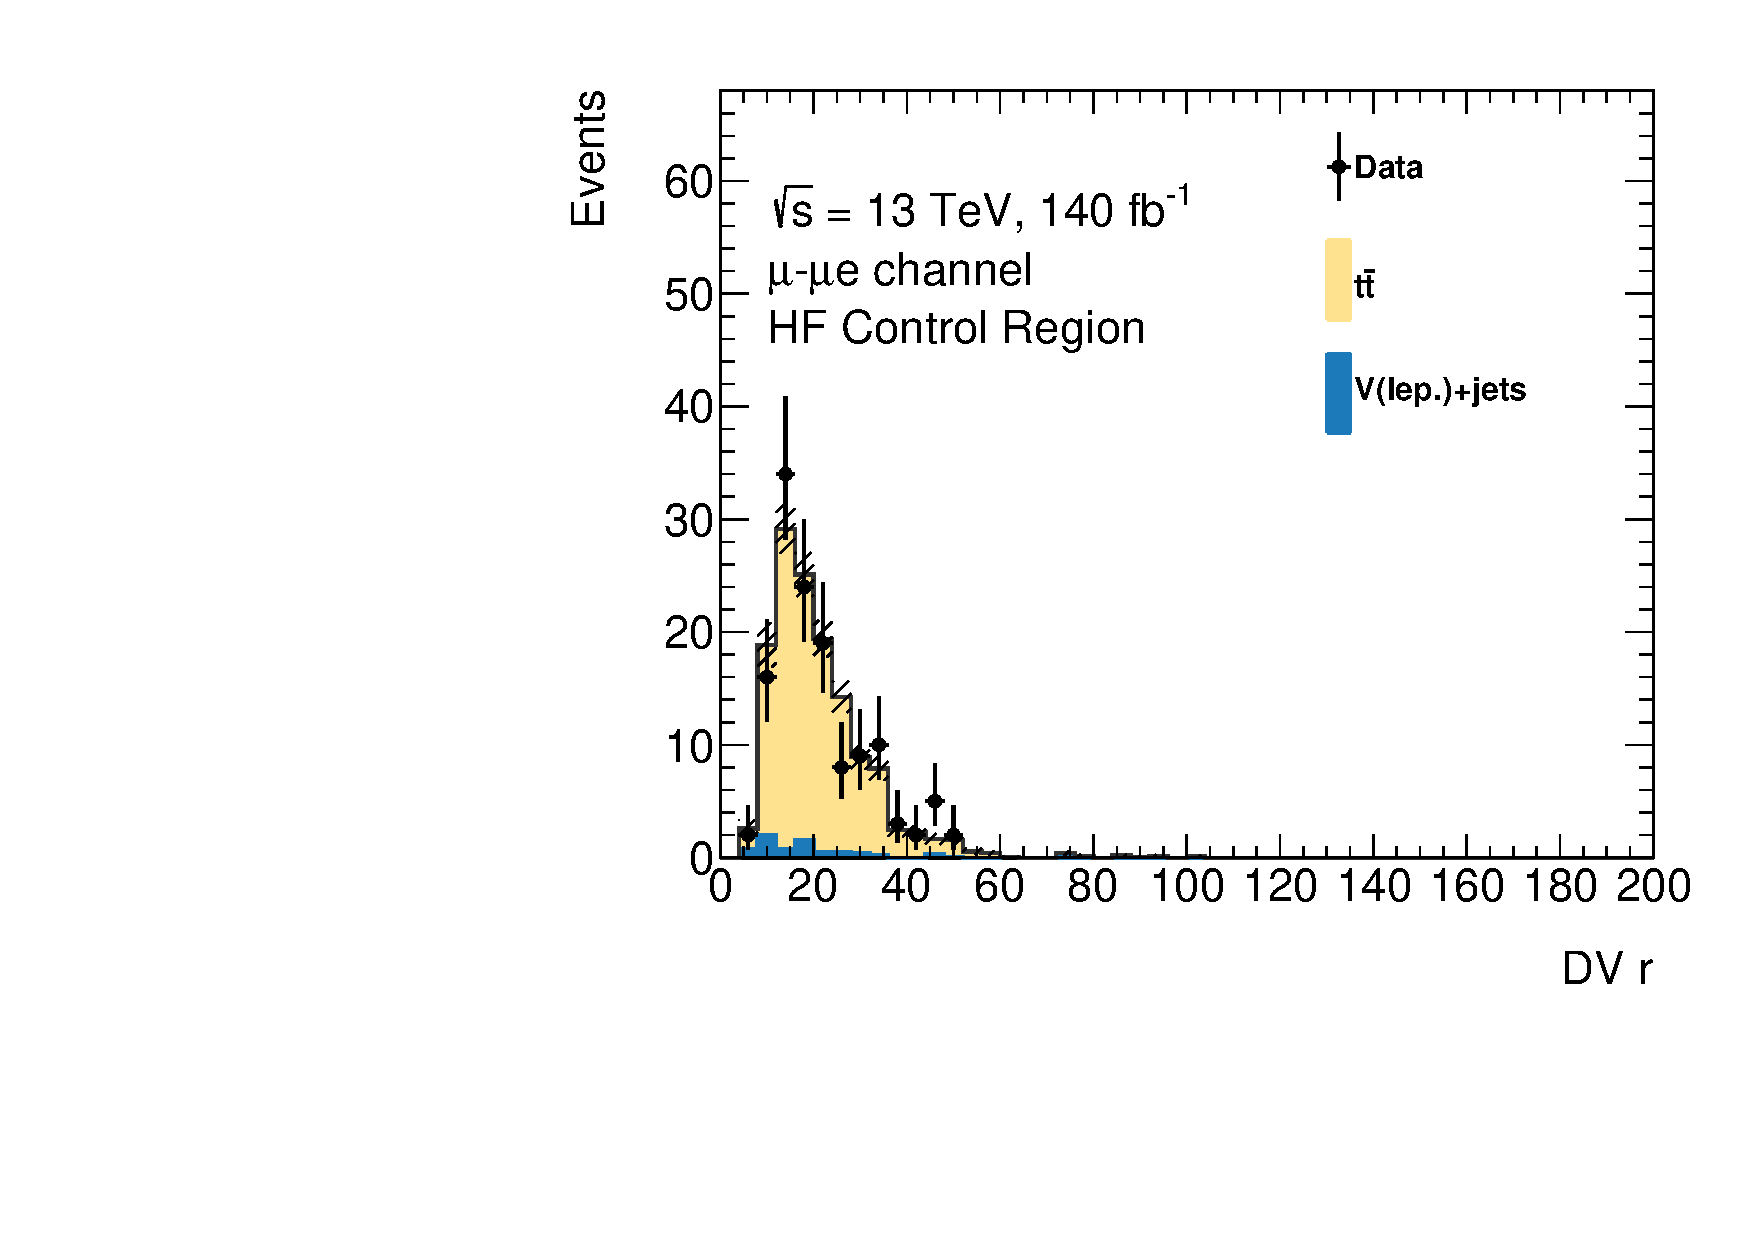
\includegraphics[width=0.24\linewidth]{figures/analysis_strategy/CR_plots/uue/DV_r.pdf}}
    \subfloat[{$\mathcal{S}$}]{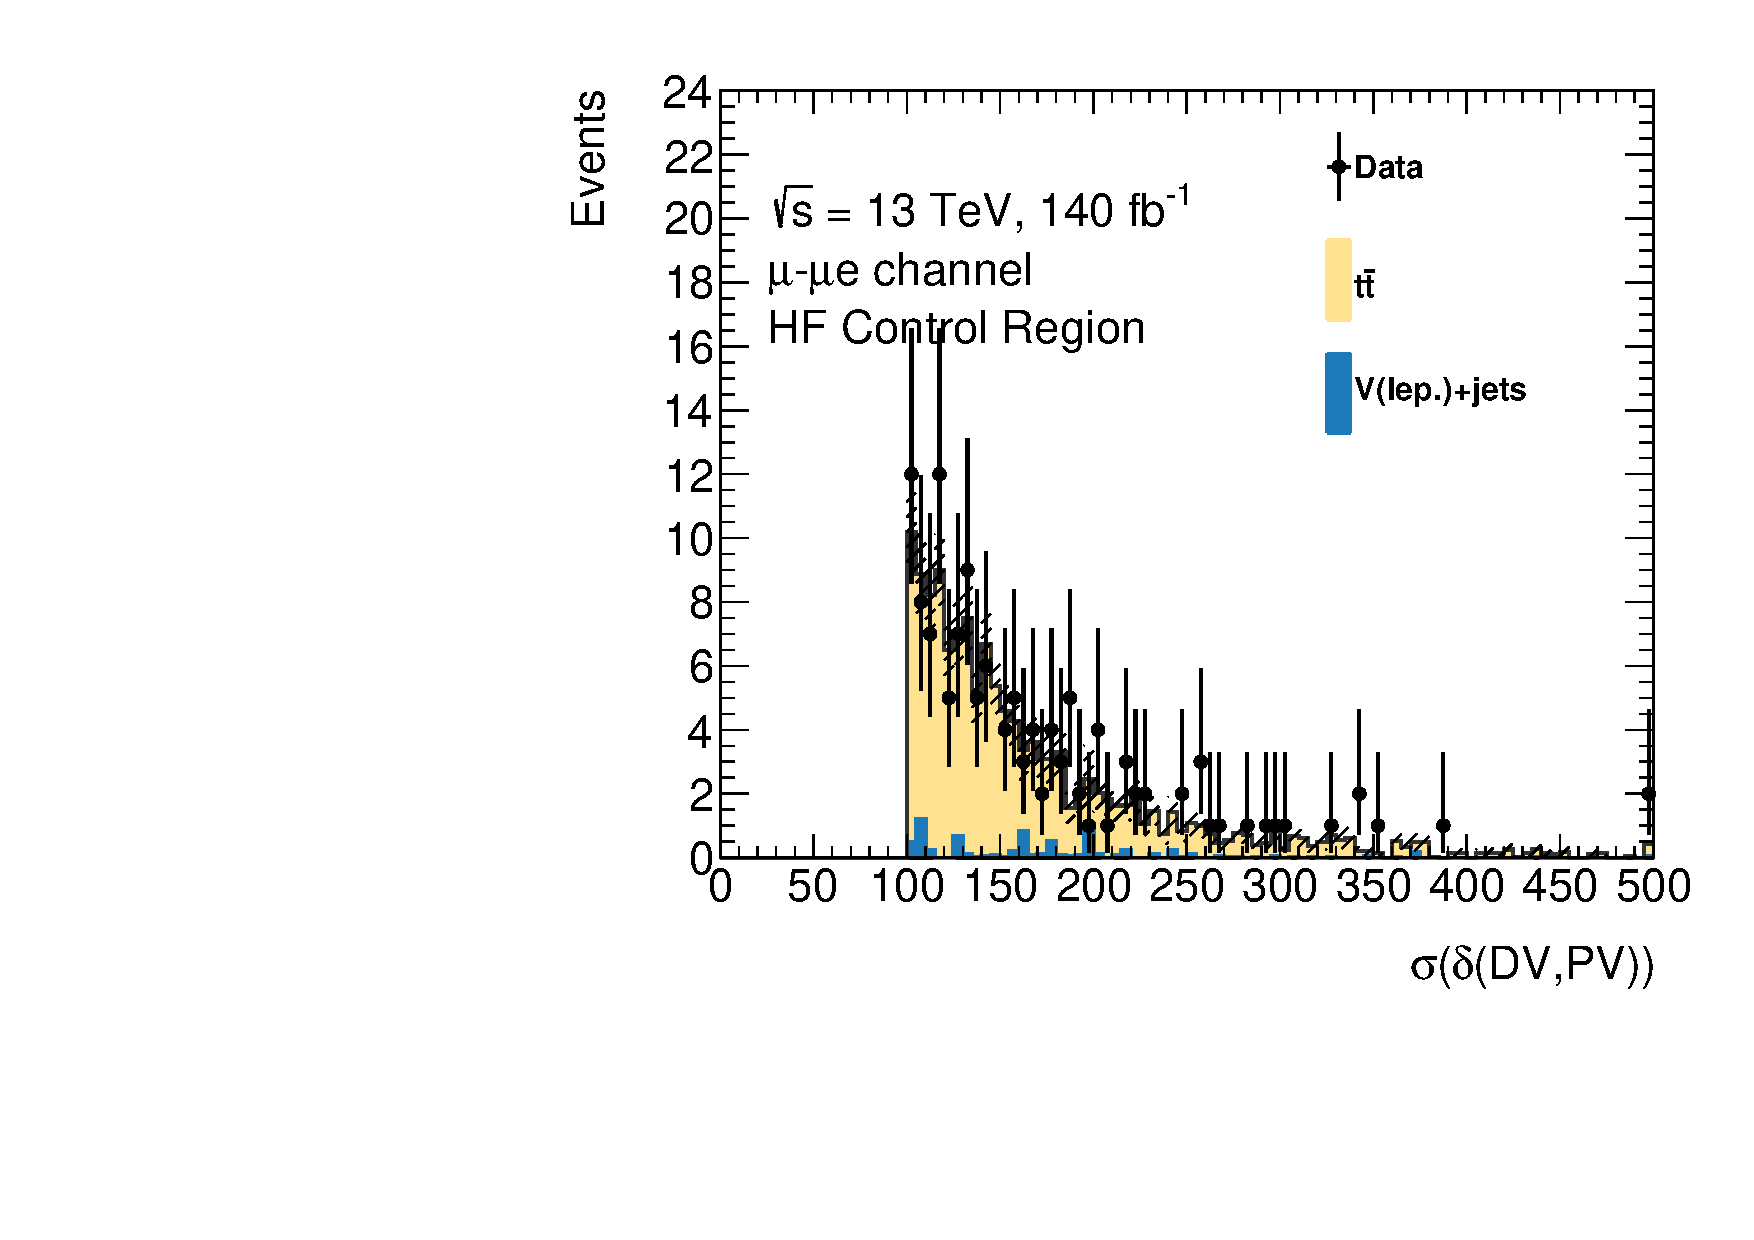
\includegraphics[width=0.24\linewidth]{figures/analysis_strategy/CR_plots/uue/DV_distFromPVsigni.pdf}}
    \subfloat[{prompt lep. \pT [GeV]}]{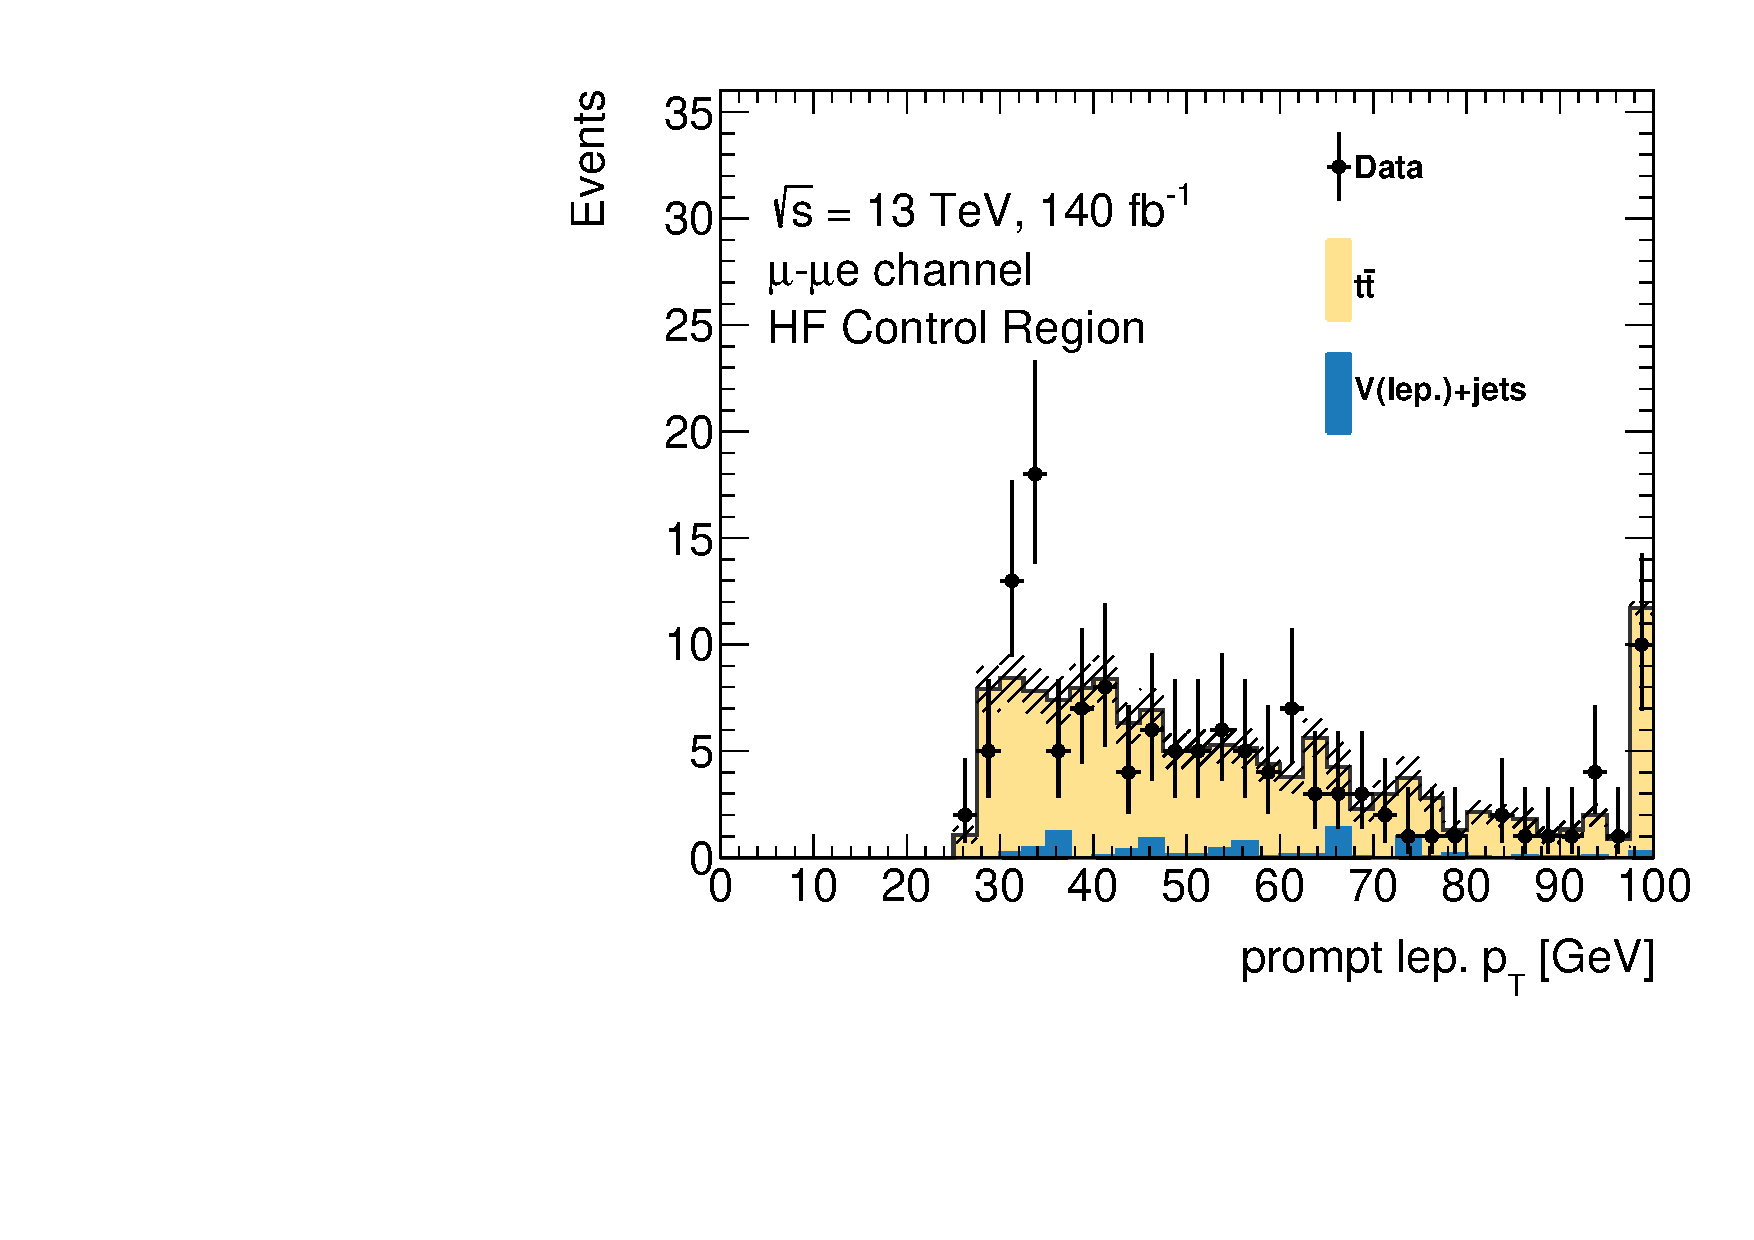
\includegraphics[width=0.24\linewidth]{figures/analysis_strategy/CR_plots/uue/prompt_lepton_pt.pdf}}\\
    \subfloat[{$\Delta R$ DV tracks}]{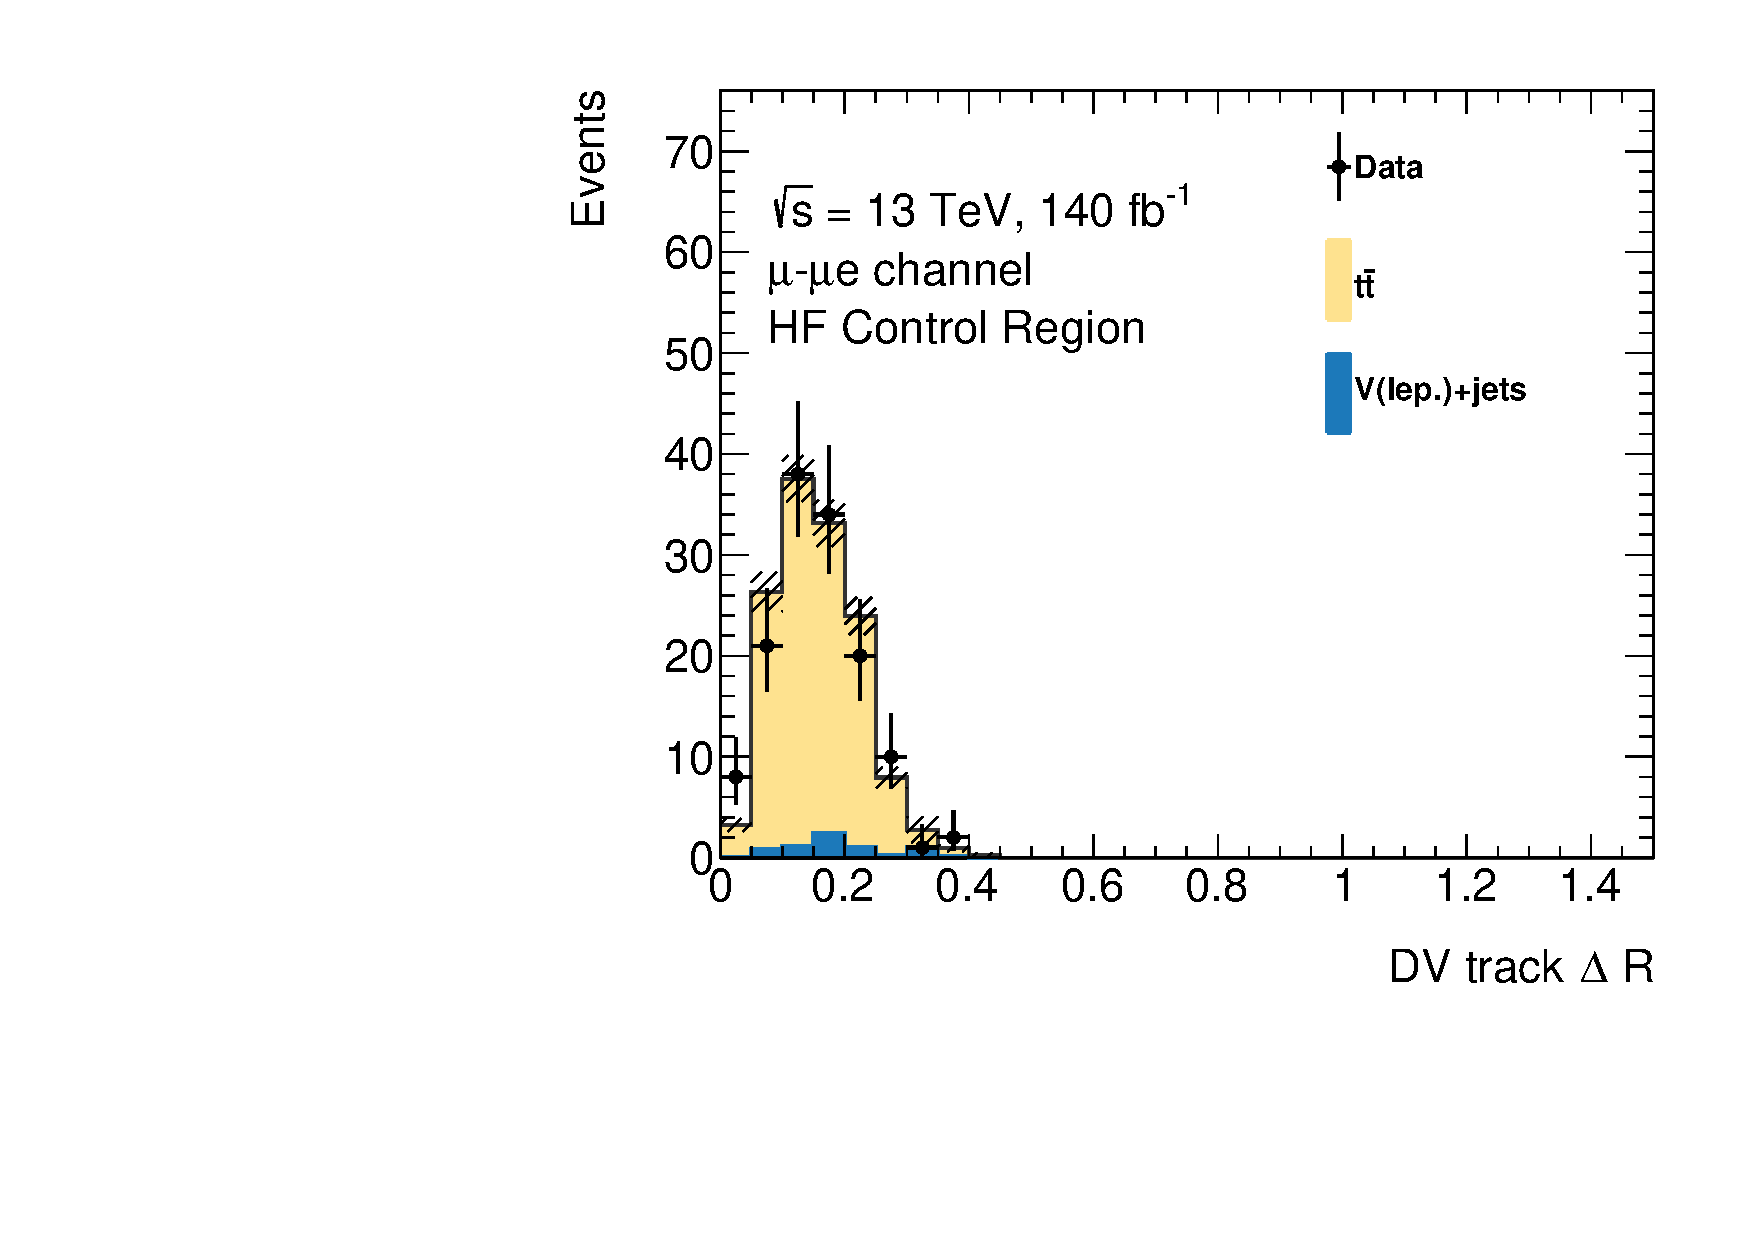
\includegraphics[width=0.24\linewidth]{figures/analysis_strategy/CR_plots/uue/DV_track_dR.pdf}}
    \subfloat[{\pT of DV tracks [GeV]}]{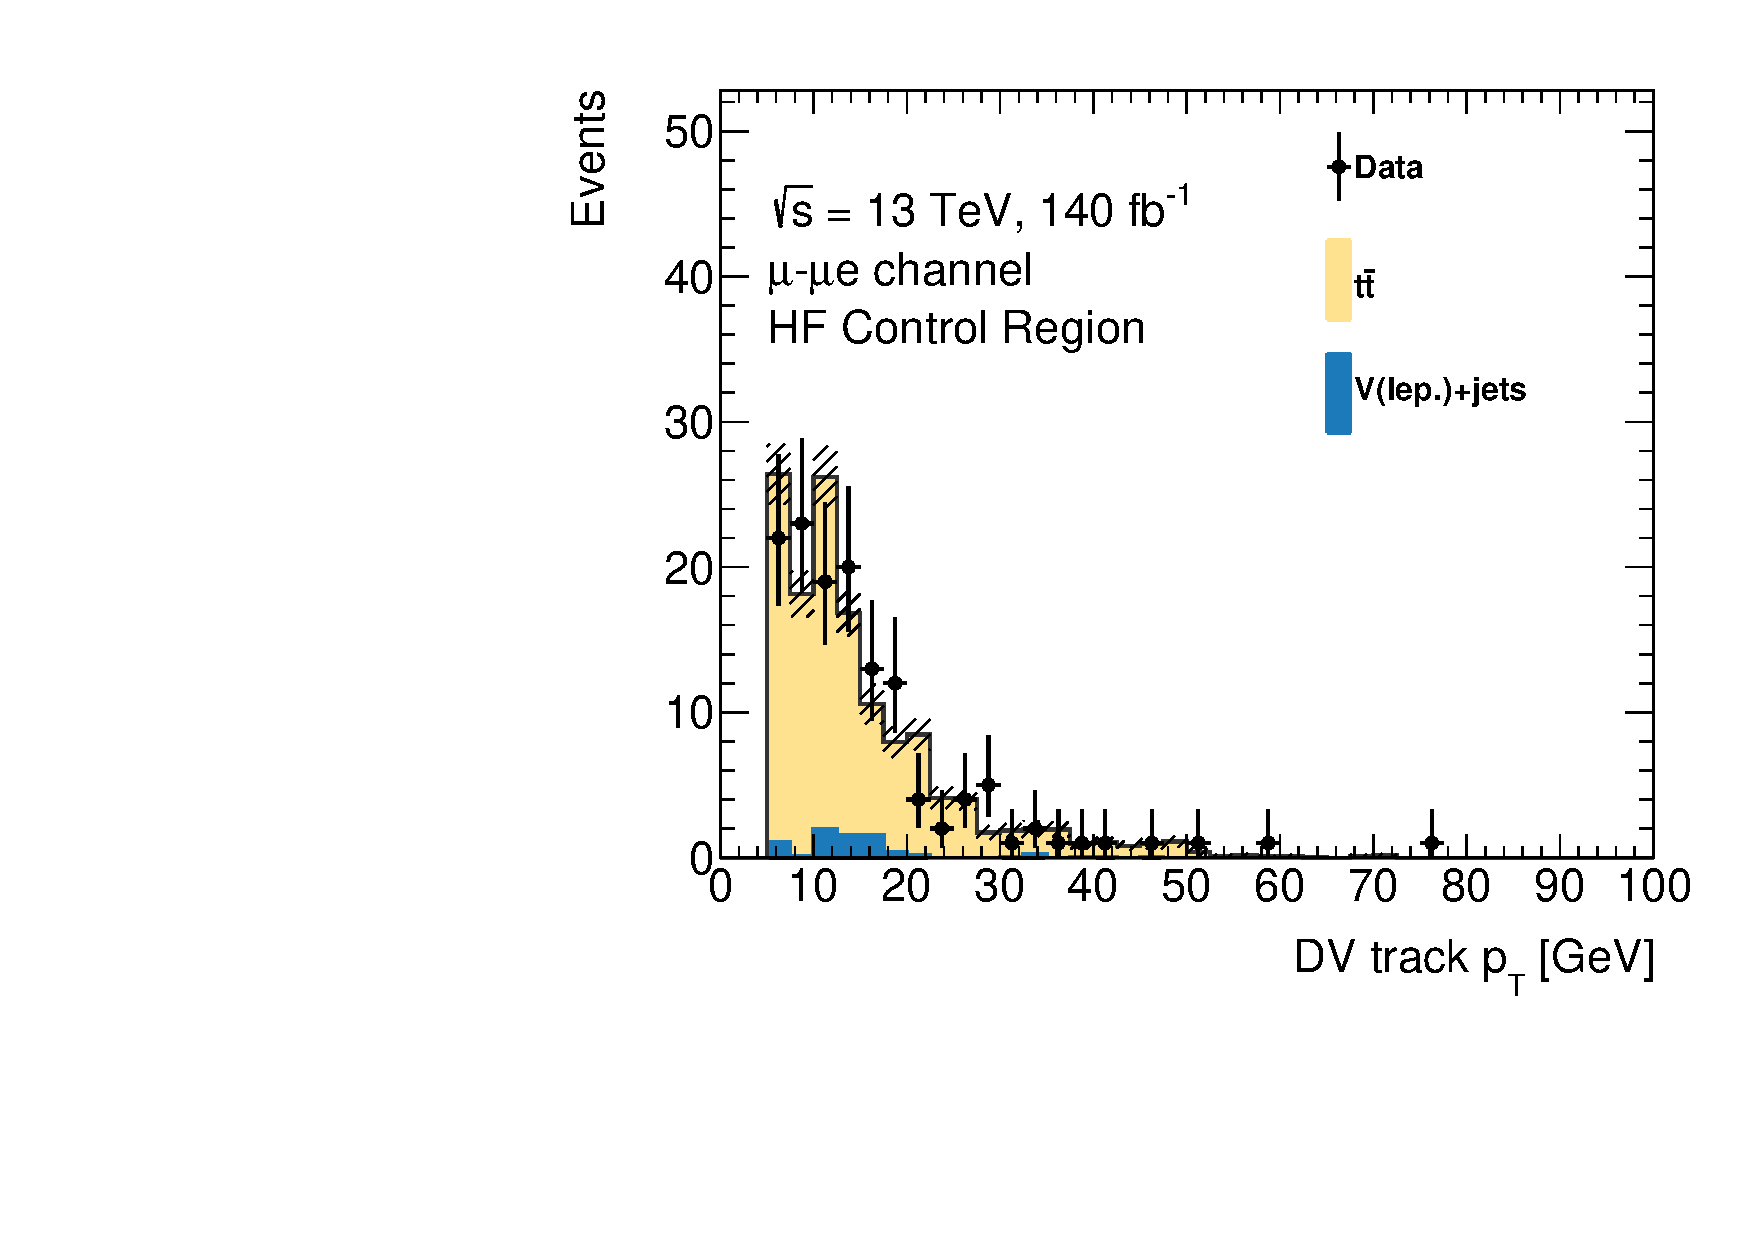
\includegraphics[width=0.24\linewidth]{figures/analysis_strategy/CR_plots/uue/DV_trk_pt.pdf}}
    \subfloat[{$\eta$ of DV tracks}]{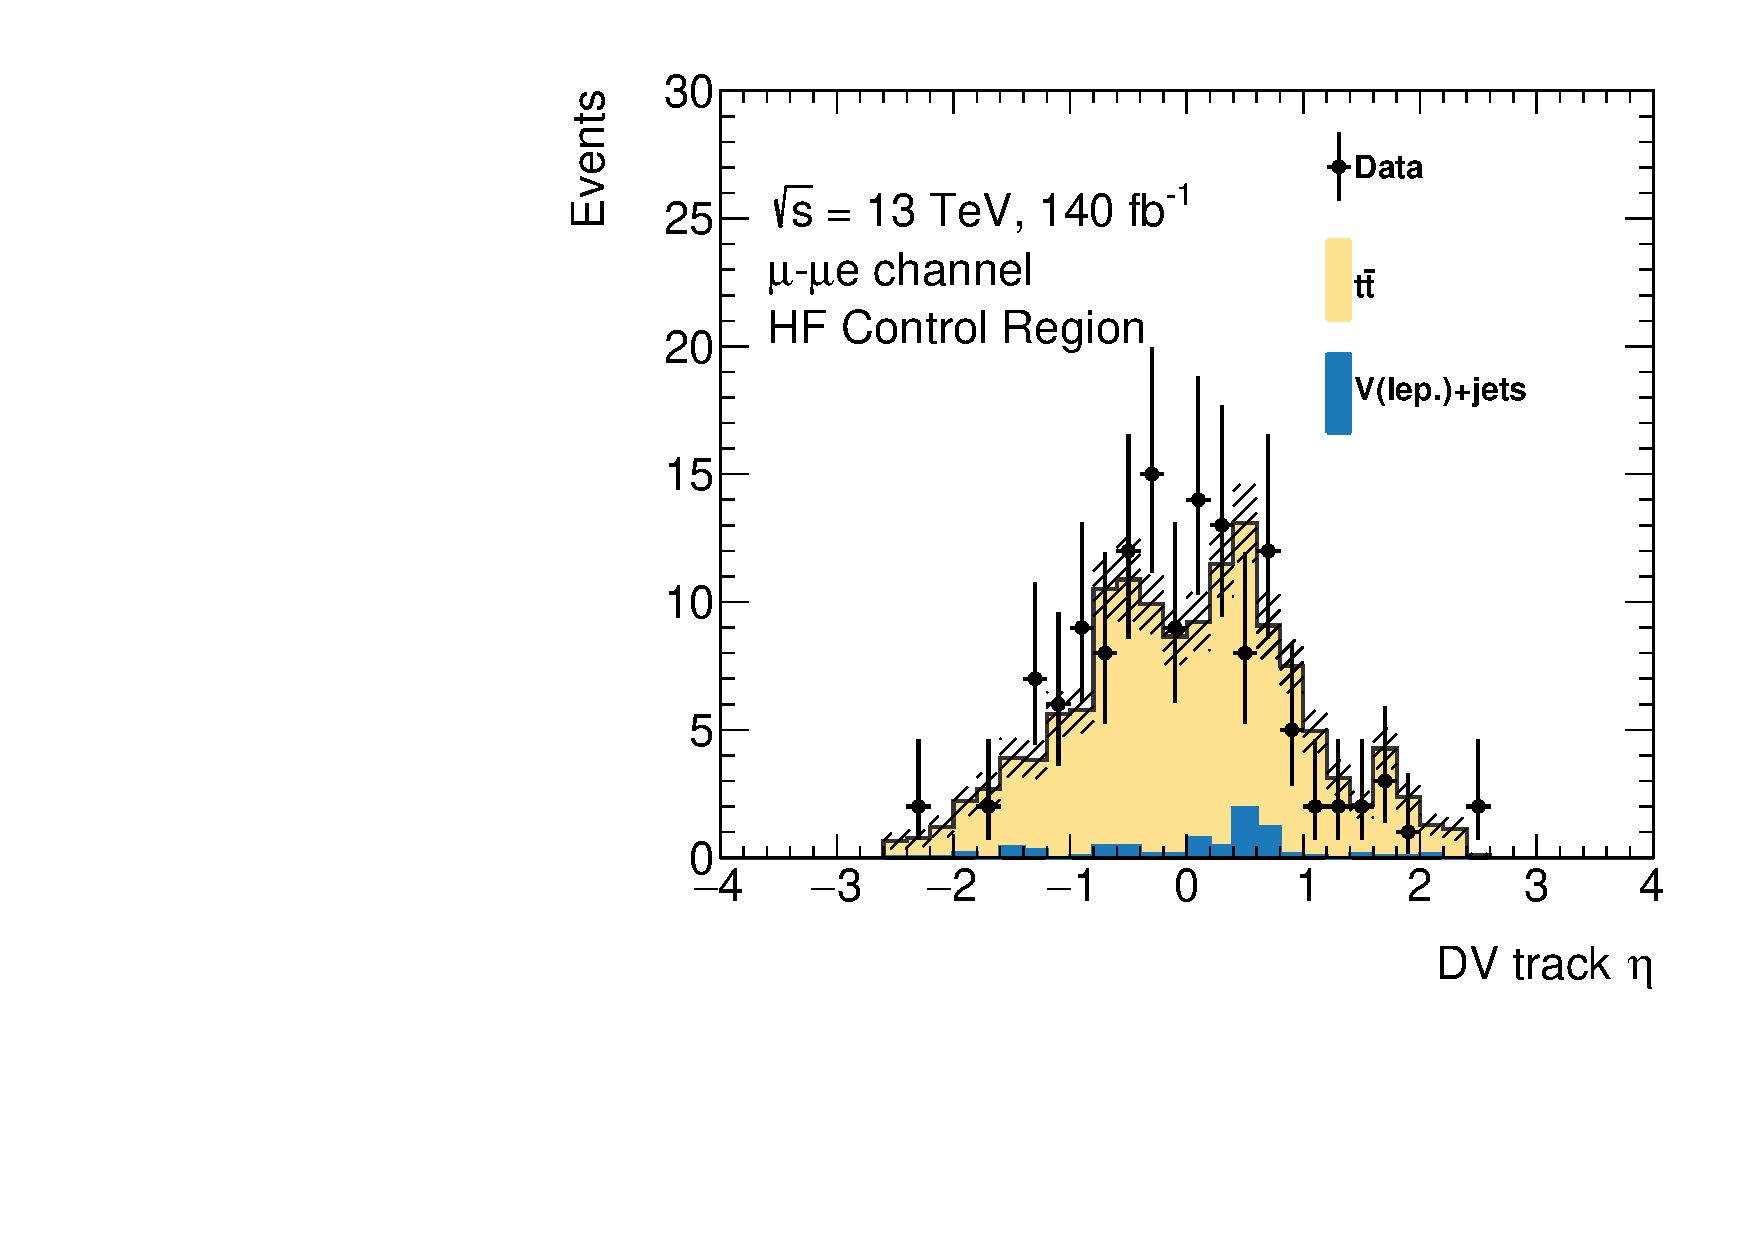
\includegraphics[width=0.24\linewidth]{figures/analysis_strategy/CR_plots/uue/DV_trk_eta.pdf}}
    \subfloat[{$d_0$ of DV tracks [mm]}]{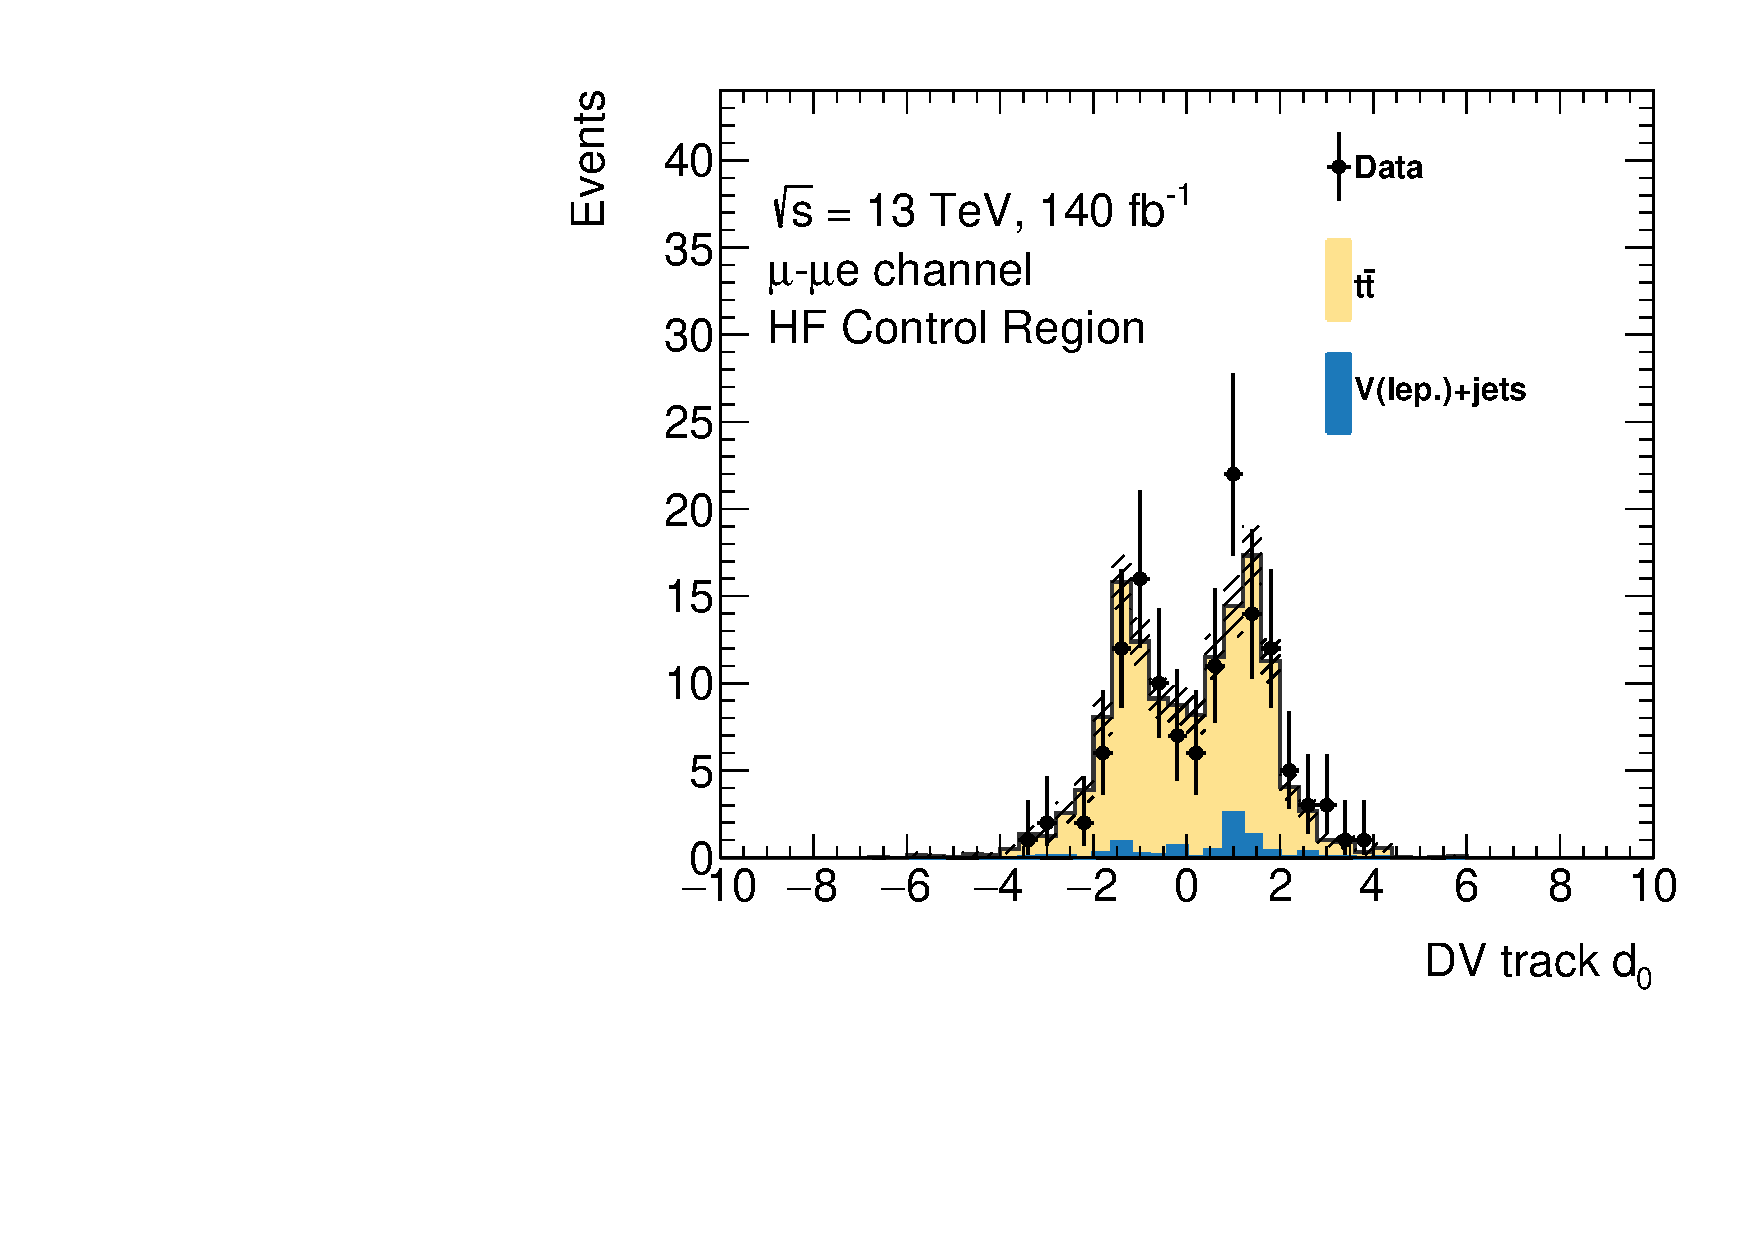
\includegraphics[width=0.24\linewidth]{figures/analysis_strategy/CR_plots/uue/DV_trk_d0.pdf}}
    \caption{Representative kinematics of the displaced vertex, tracks in the displaced vertex, and of the prompt lepton measured in ATLAS data and modeled by MC simulations in the \uue Heavy Flavor Control Region.}
    \label{fig:cr_plots_uue}
\end{figure}

\begin{figure}[!ht]
    \centering
    \subfloat[{\mdv [GeV]}]{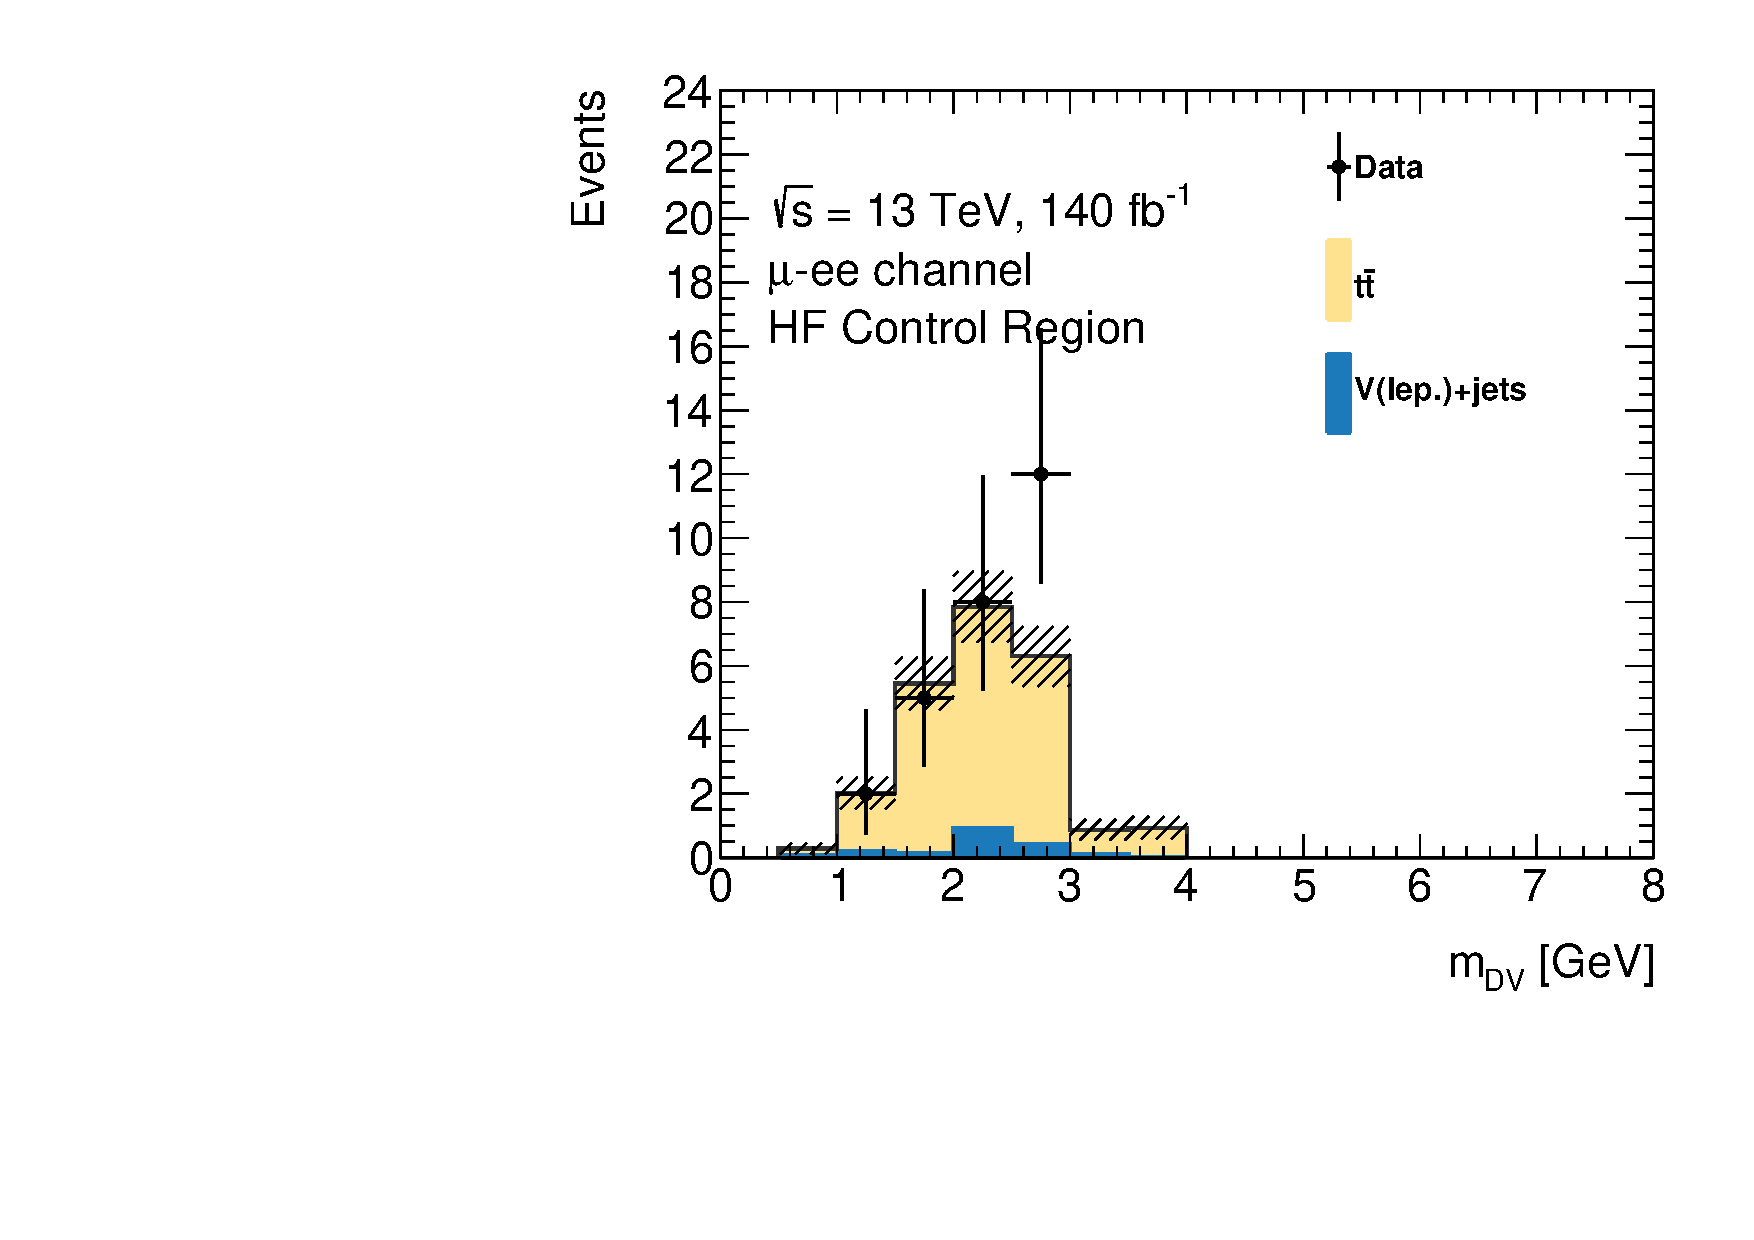
\includegraphics[width=0.24\linewidth]{figures/analysis_strategy/CR_plots/uee/DV_mass.pdf}}
    \subfloat[{$r_\mathrm{DV}$ [mm]}]{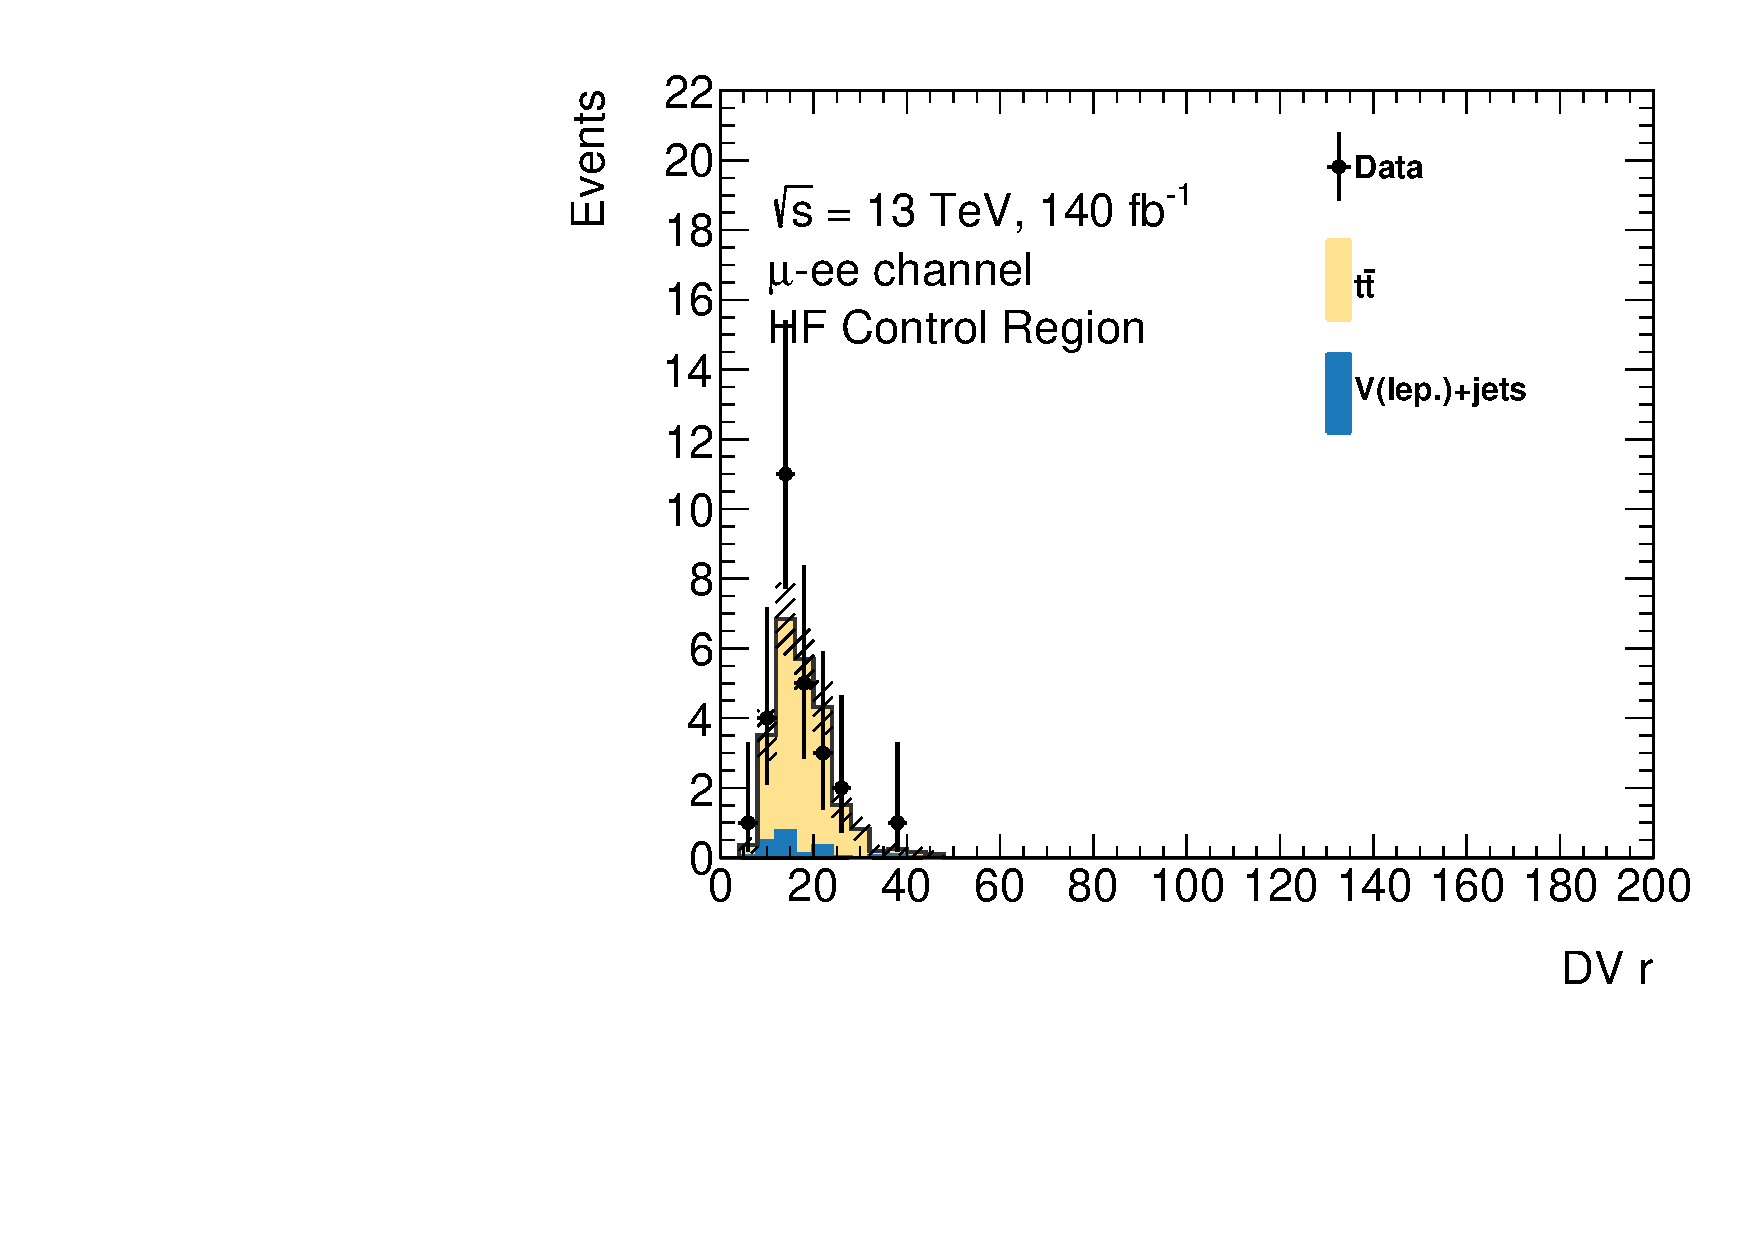
\includegraphics[width=0.24\linewidth]{figures/analysis_strategy/CR_plots/uee/DV_r.pdf}}
    \subfloat[{$\mathcal{S}$}]{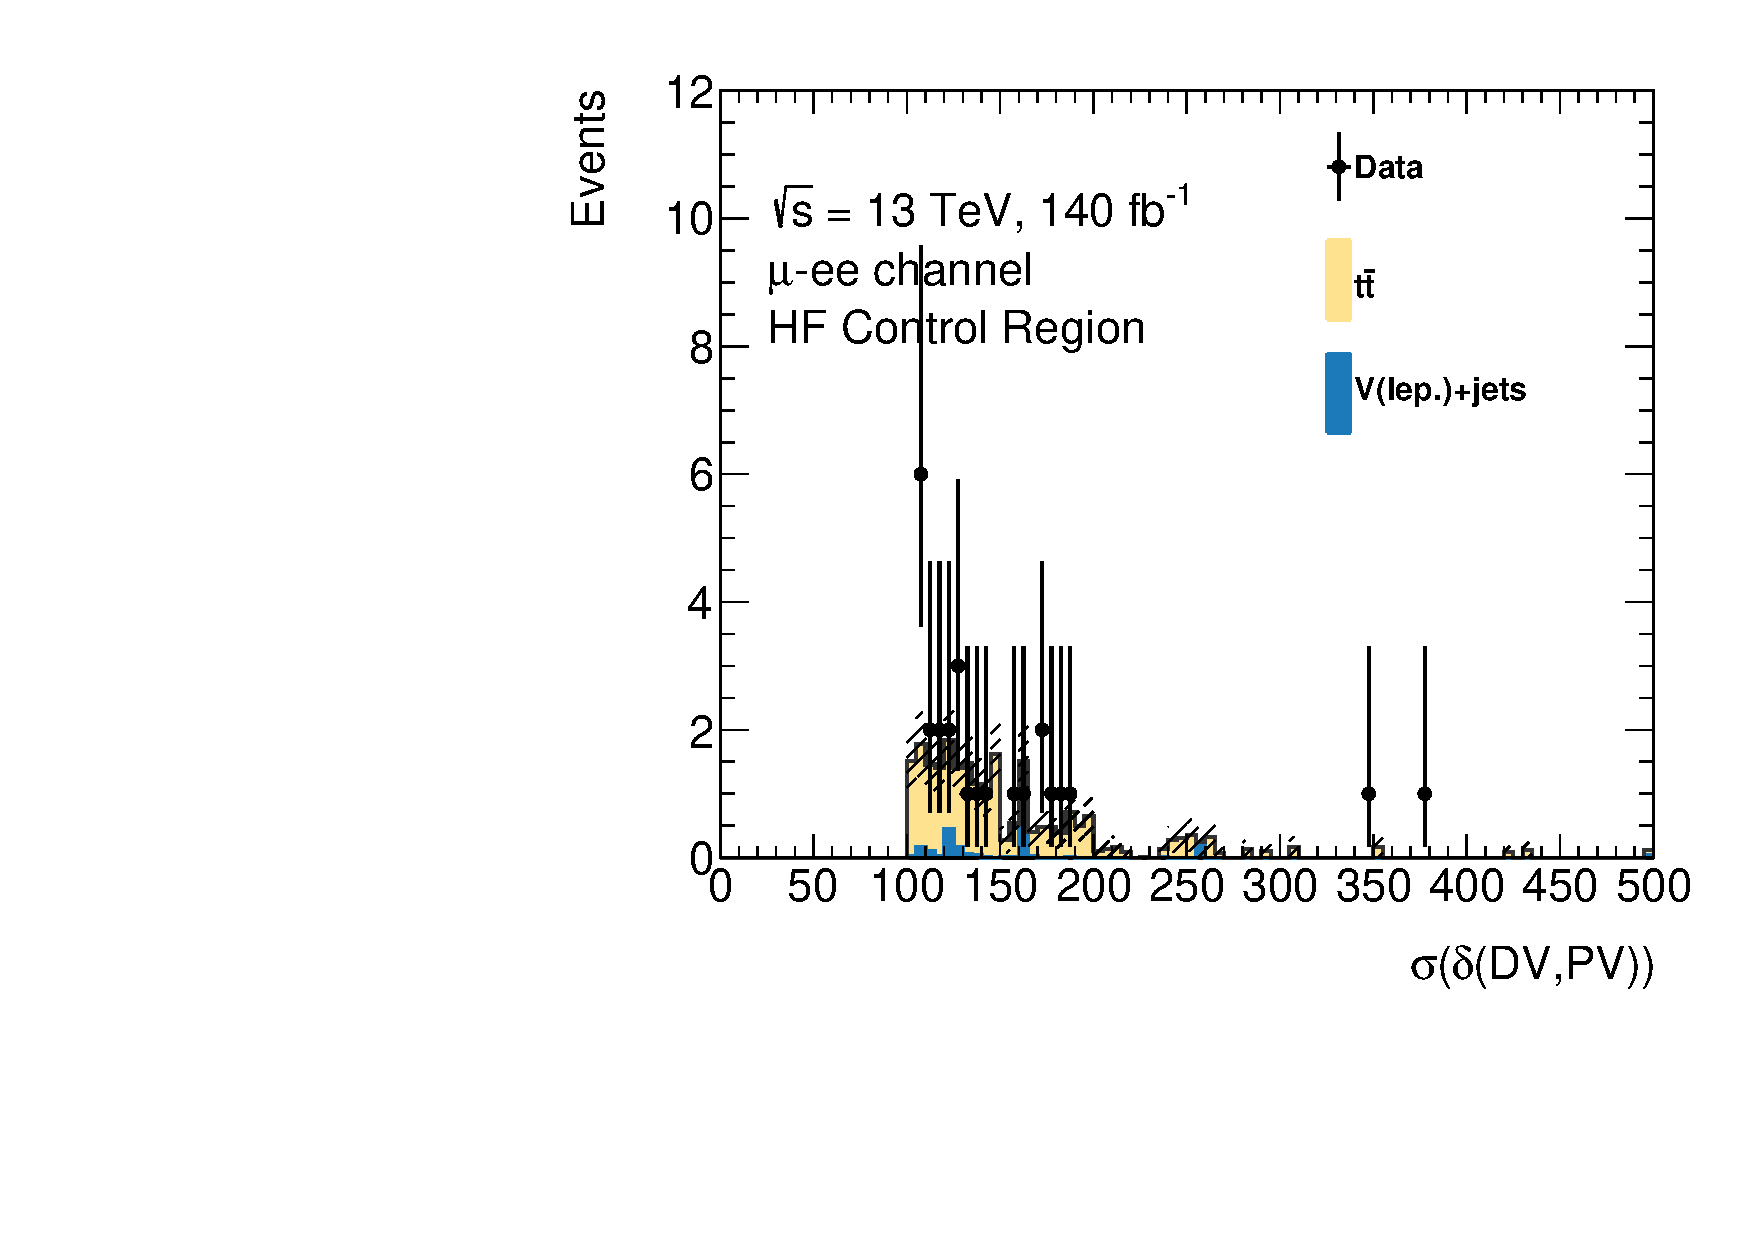
\includegraphics[width=0.24\linewidth]{figures/analysis_strategy/CR_plots/uee/DV_distFromPVsigni.pdf}}
    \subfloat[{prompt lep. \pT [GeV]}]{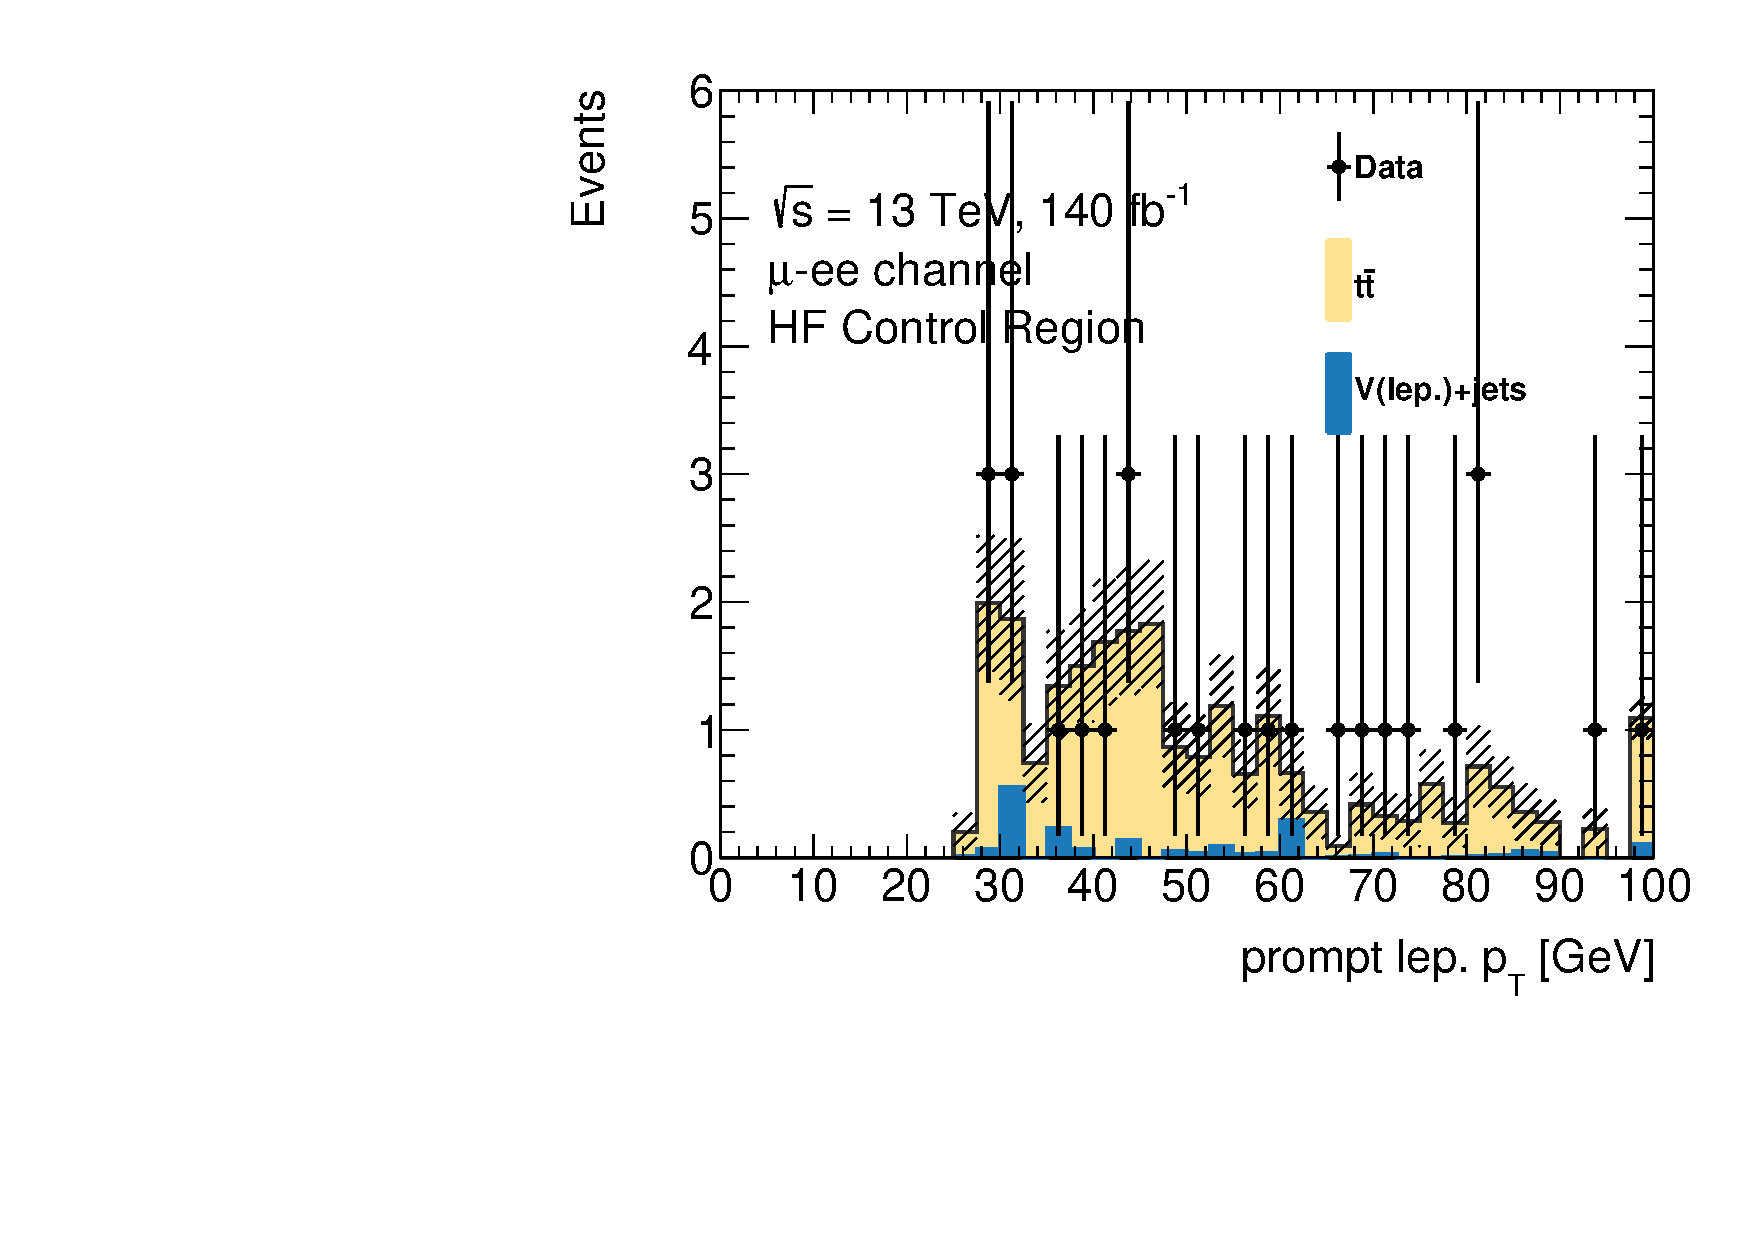
\includegraphics[width=0.24\linewidth]{figures/analysis_strategy/CR_plots/uee/prompt_lepton_pt.pdf}}\\
    \subfloat[{$\Delta R$ DV tracks}]{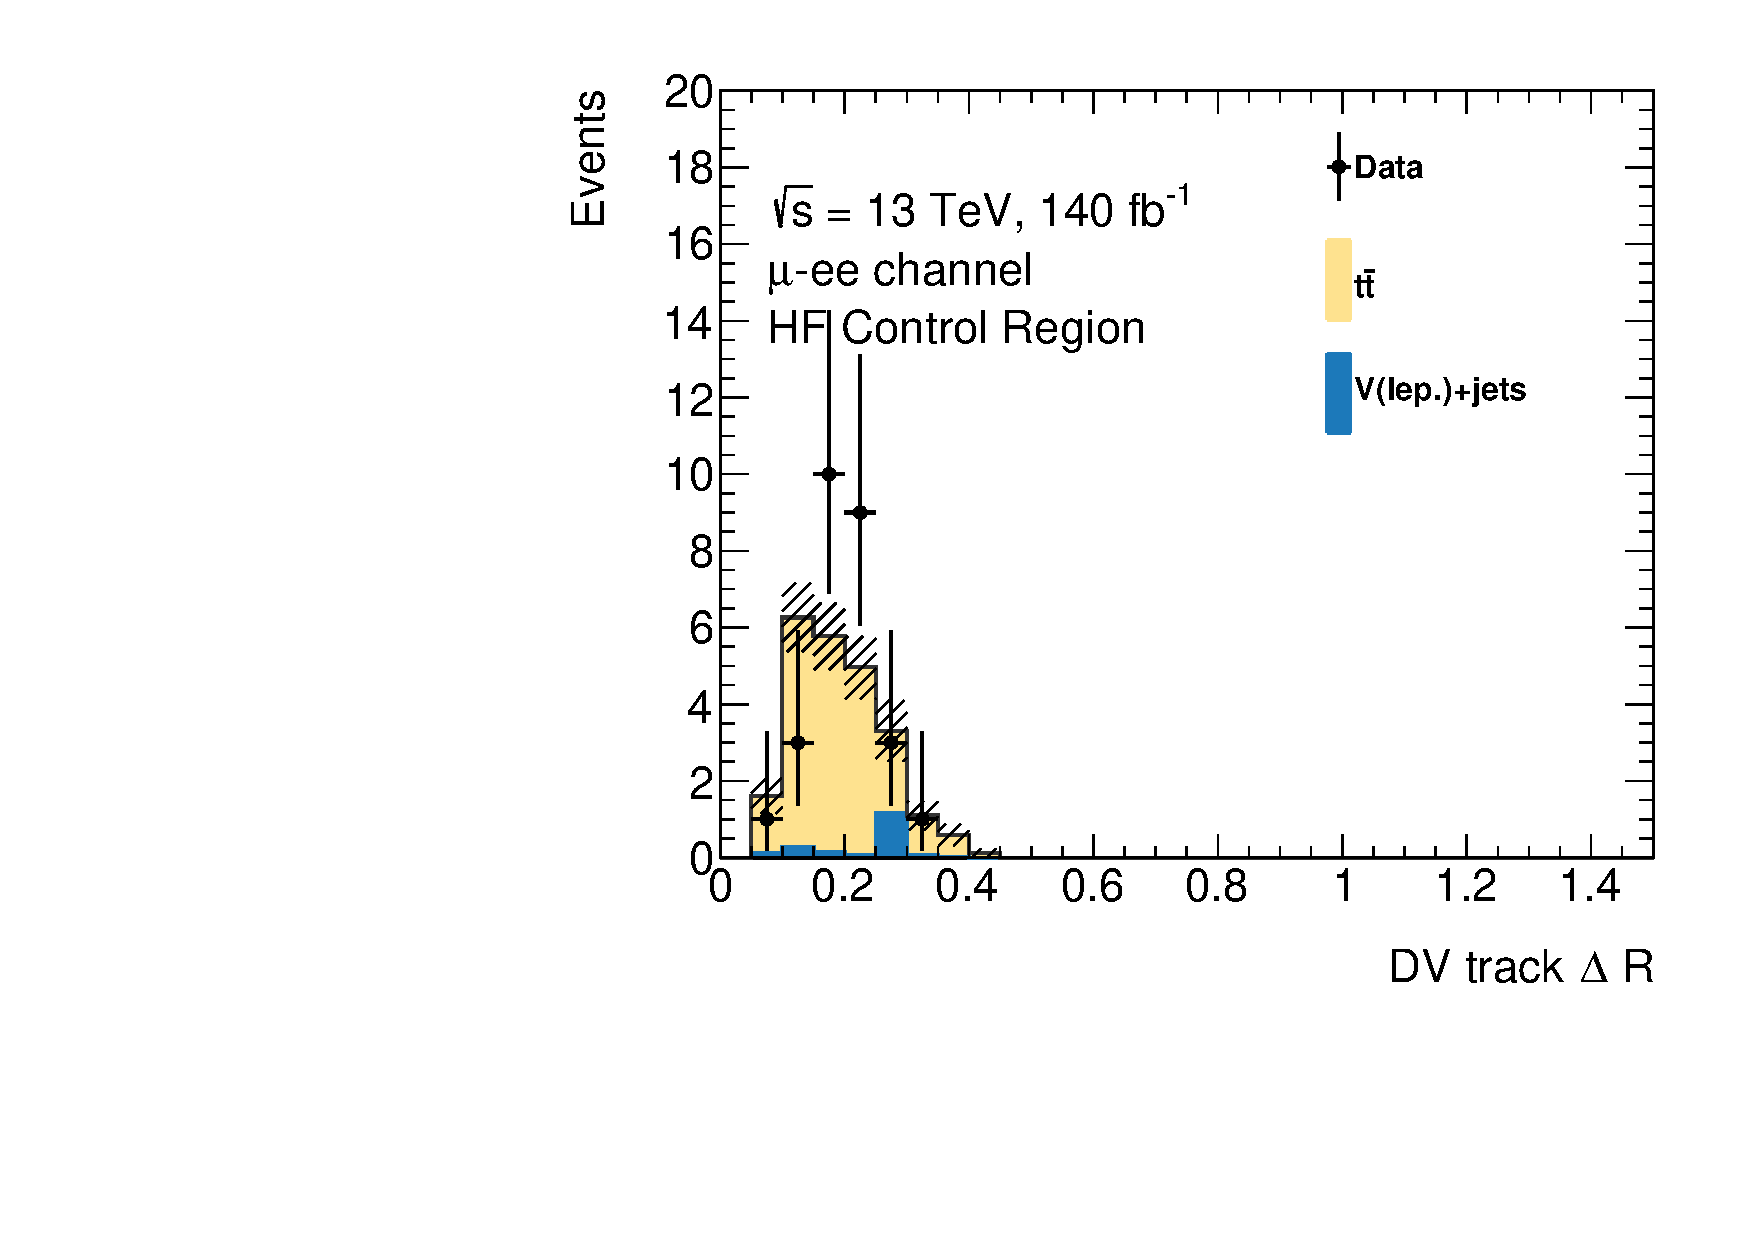
\includegraphics[width=0.24\linewidth]{figures/analysis_strategy/CR_plots/uee/DV_track_dR.pdf}}
    \subfloat[{\pT of DV tracks [GeV]}]{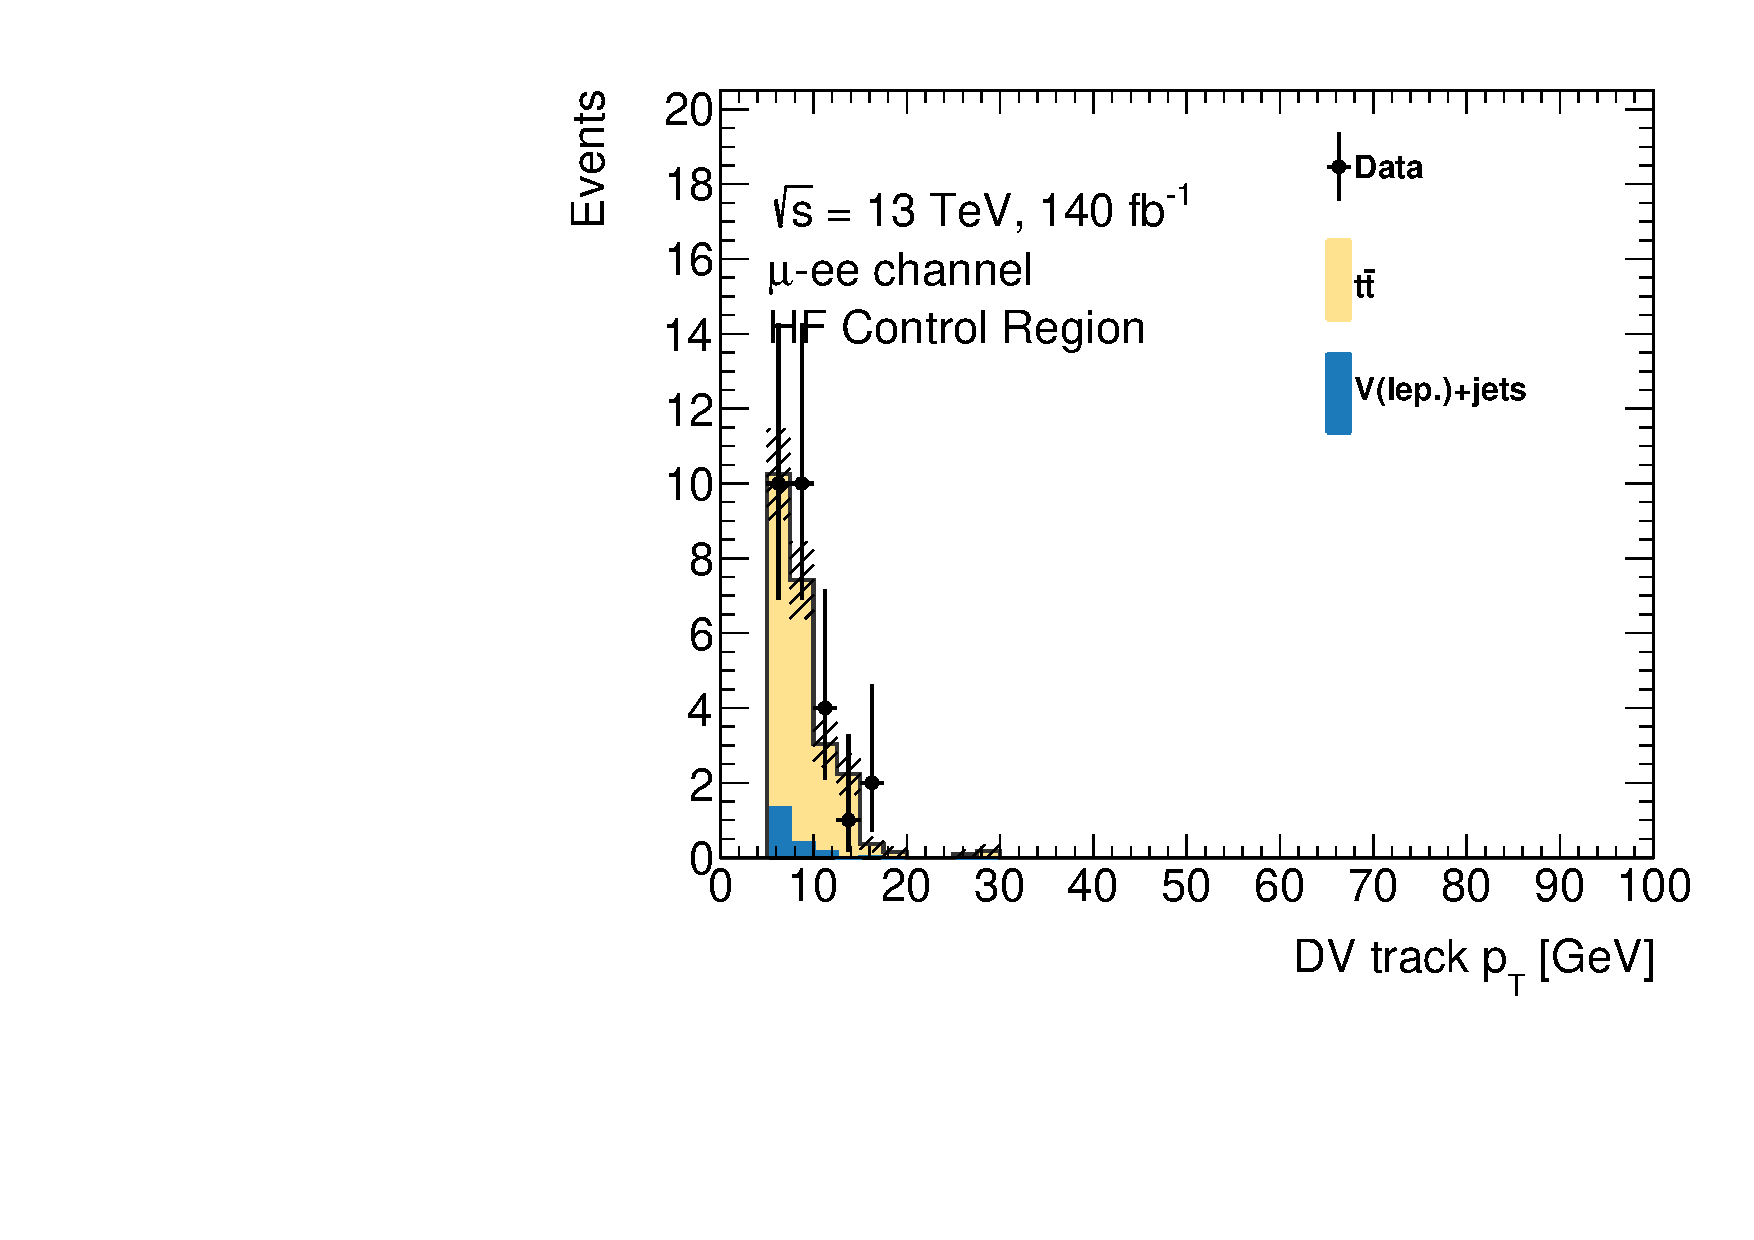
\includegraphics[width=0.24\linewidth]{figures/analysis_strategy/CR_plots/uee/DV_trk_pt.pdf}}
    \subfloat[{$\eta$ of DV tracks}]{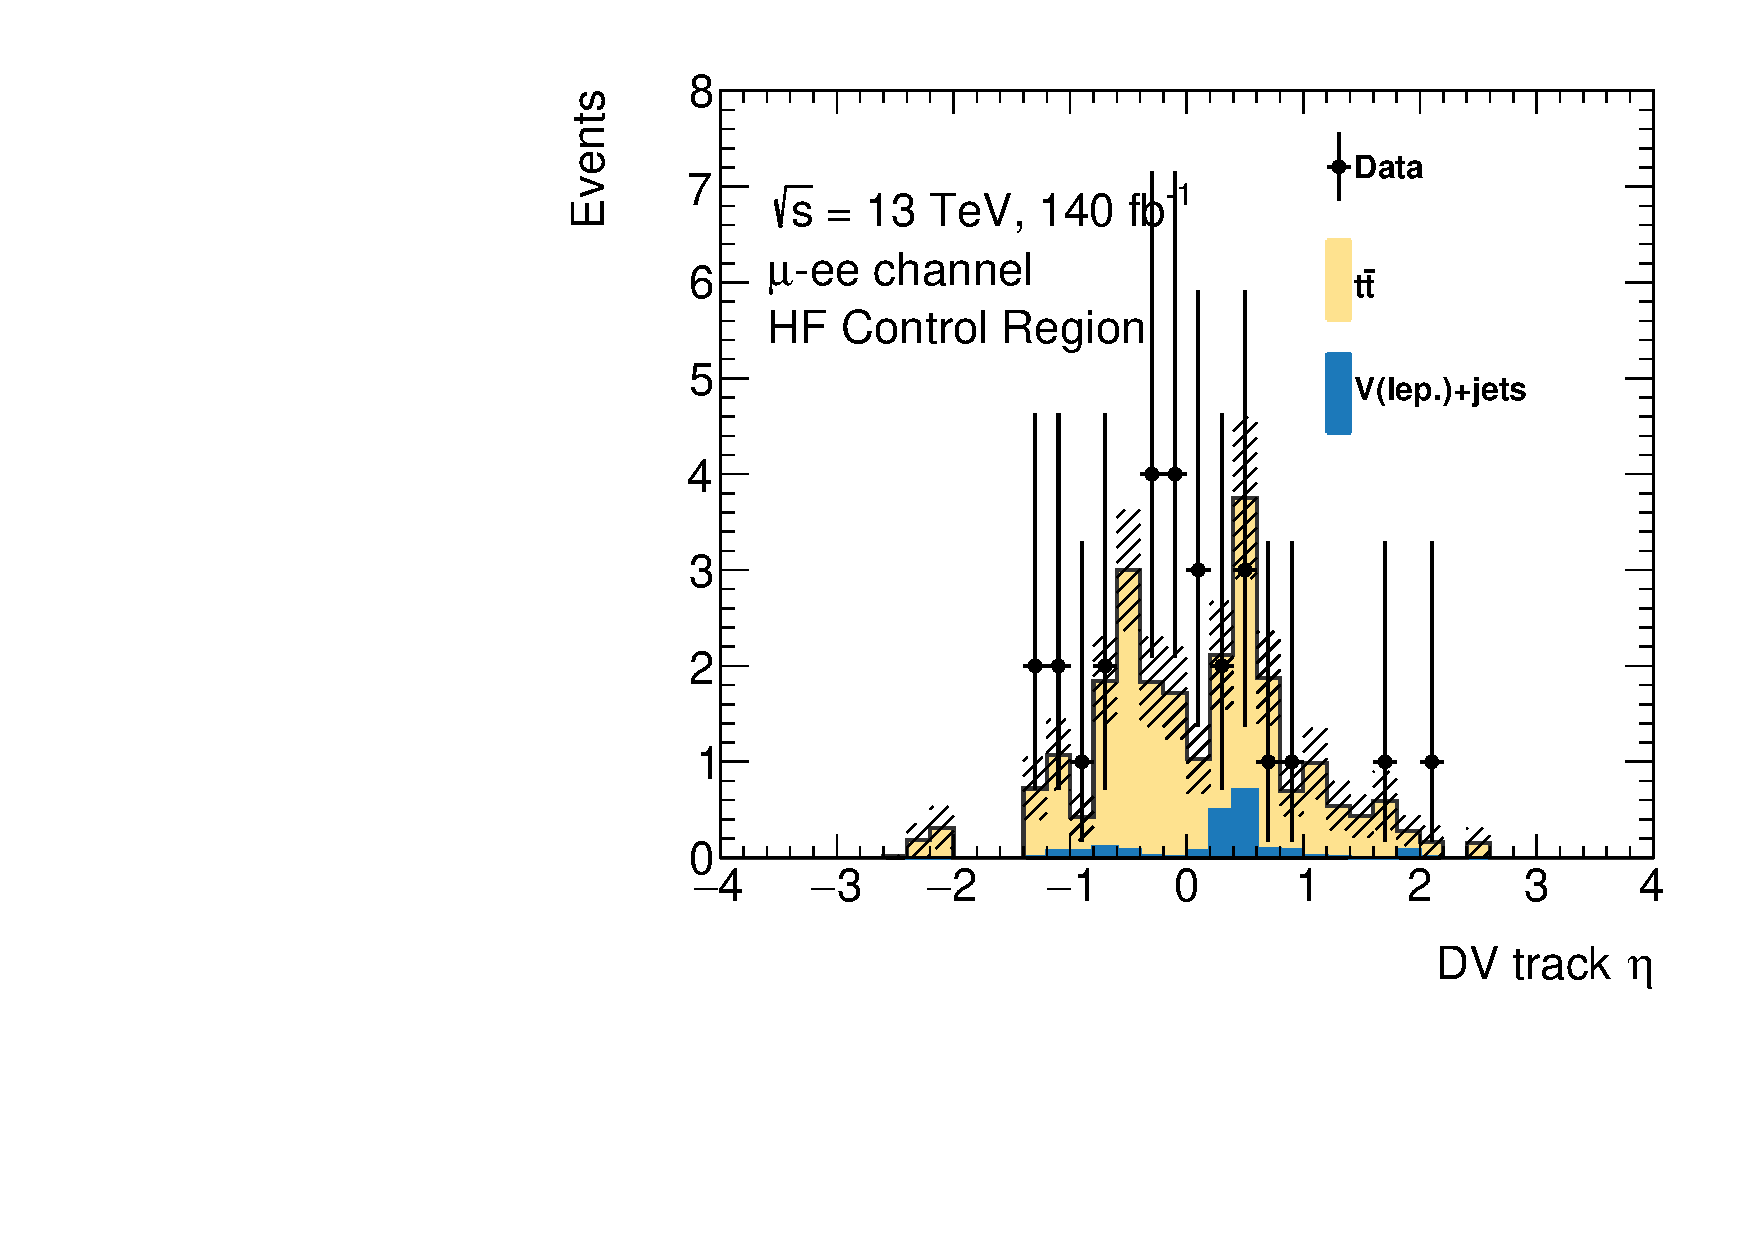
\includegraphics[width=0.24\linewidth]{figures/analysis_strategy/CR_plots/uee/DV_trk_eta.pdf}}
    \subfloat[{$d_0$ of DV tracks [mm]}]{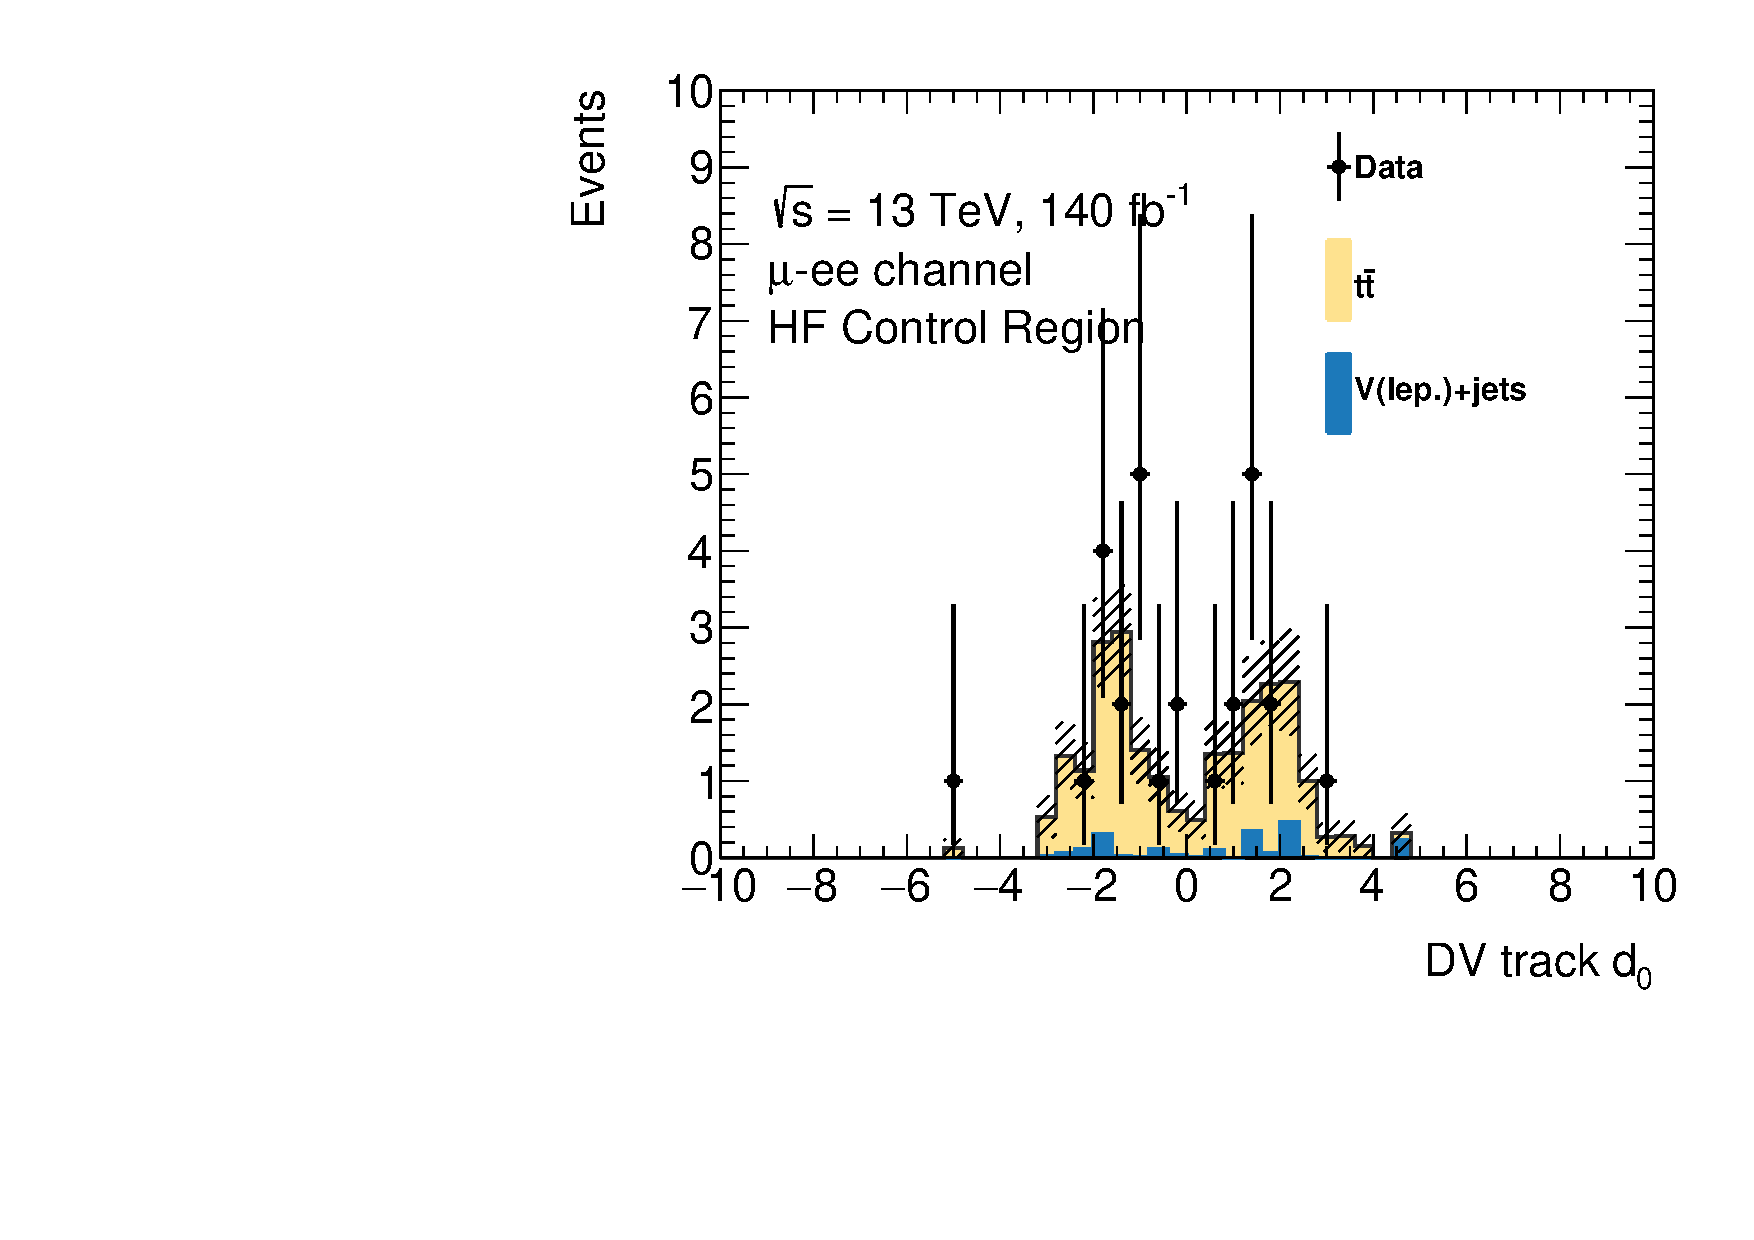
\includegraphics[width=0.24\linewidth]{figures/analysis_strategy/CR_plots/uee/DV_trk_d0.pdf}}
    \caption{Representative kinematics of the displaced vertex, tracks in the displaced vertex, and of the prompt lepton measured in ATLAS data and modeled by MC simulations in the \uee Heavy Flavor Control Region.}
    \label{fig:cr_plots_uee}
\end{figure}

\begin{figure}[!ht]
    \centering
    \subfloat[{\mdv [GeV]}]{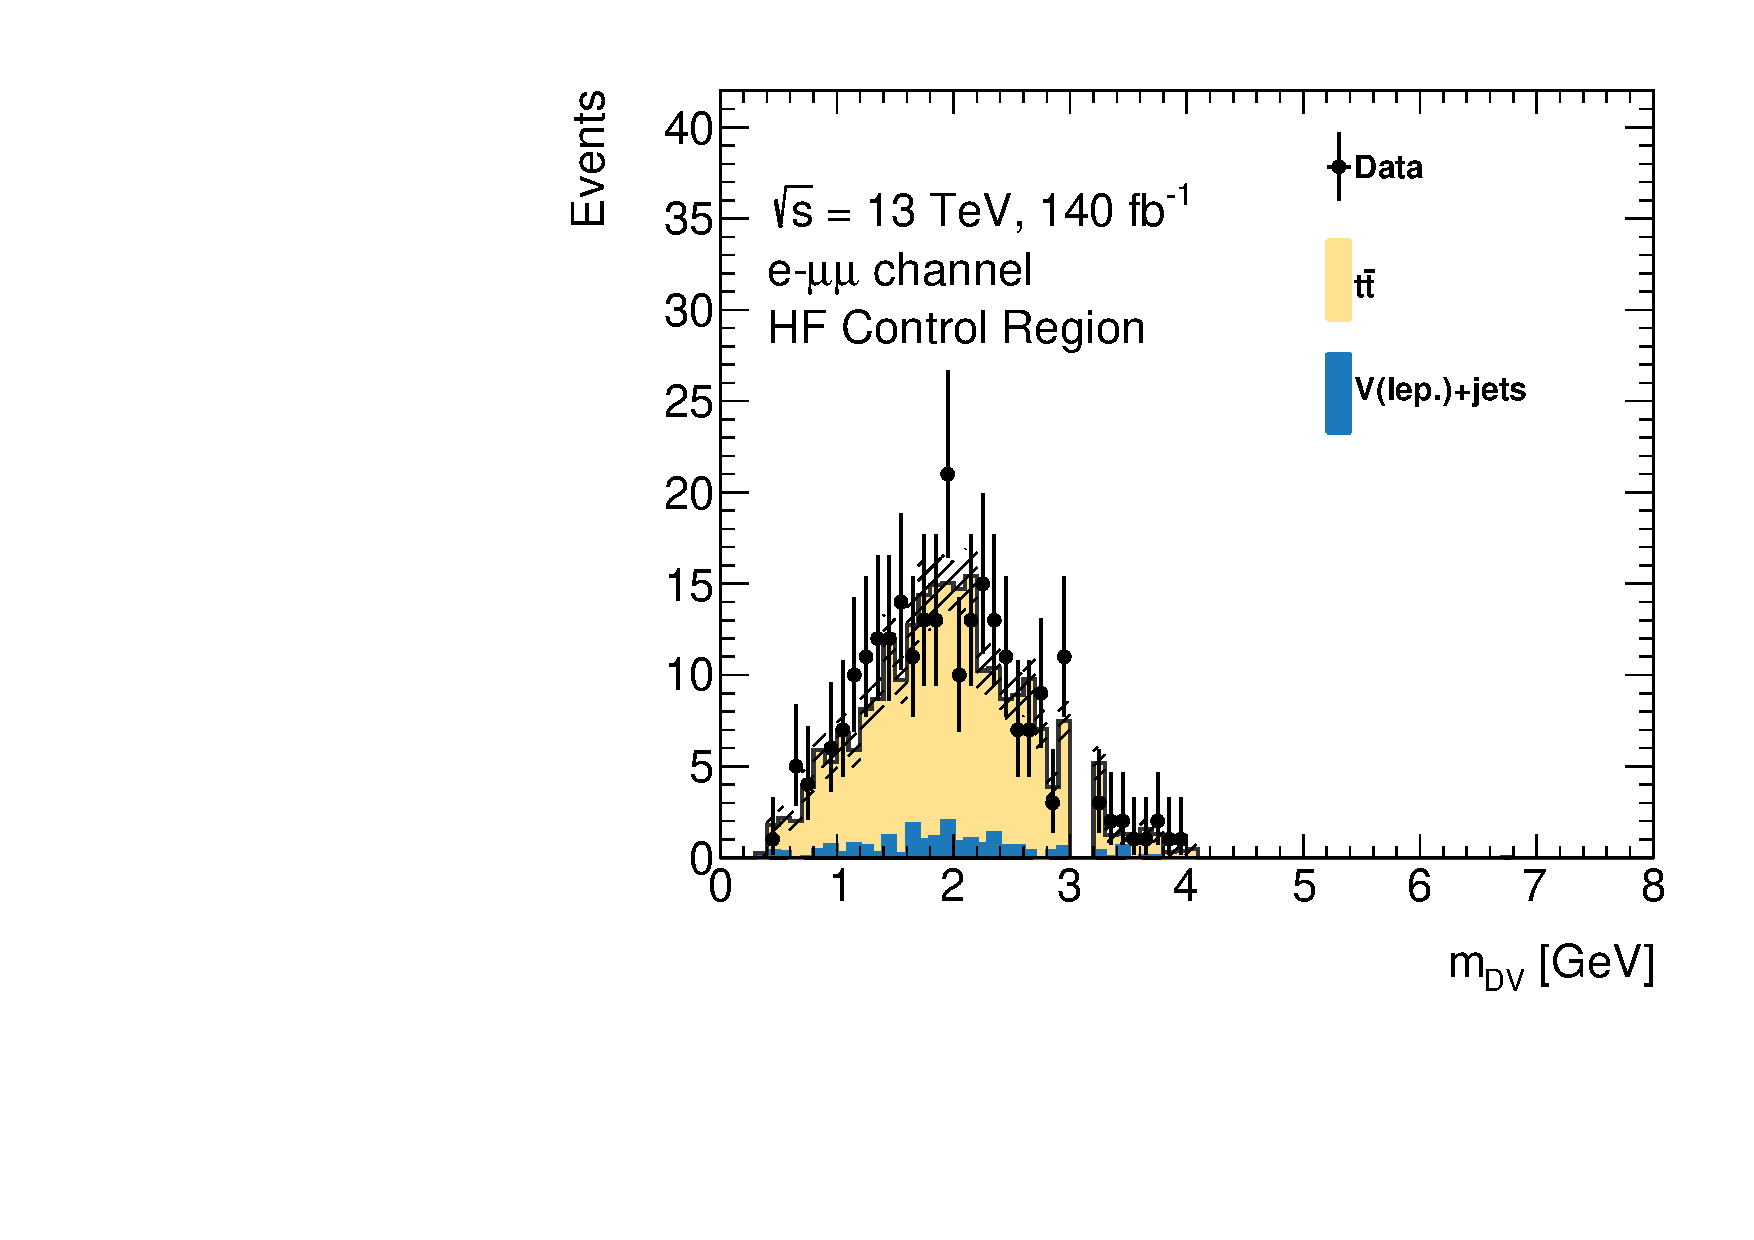
\includegraphics[width=0.24\linewidth]{figures/analysis_strategy/CR_plots/euu/DV_mass.pdf}}
    \subfloat[{$r_\mathrm{DV}$ [mm]}]{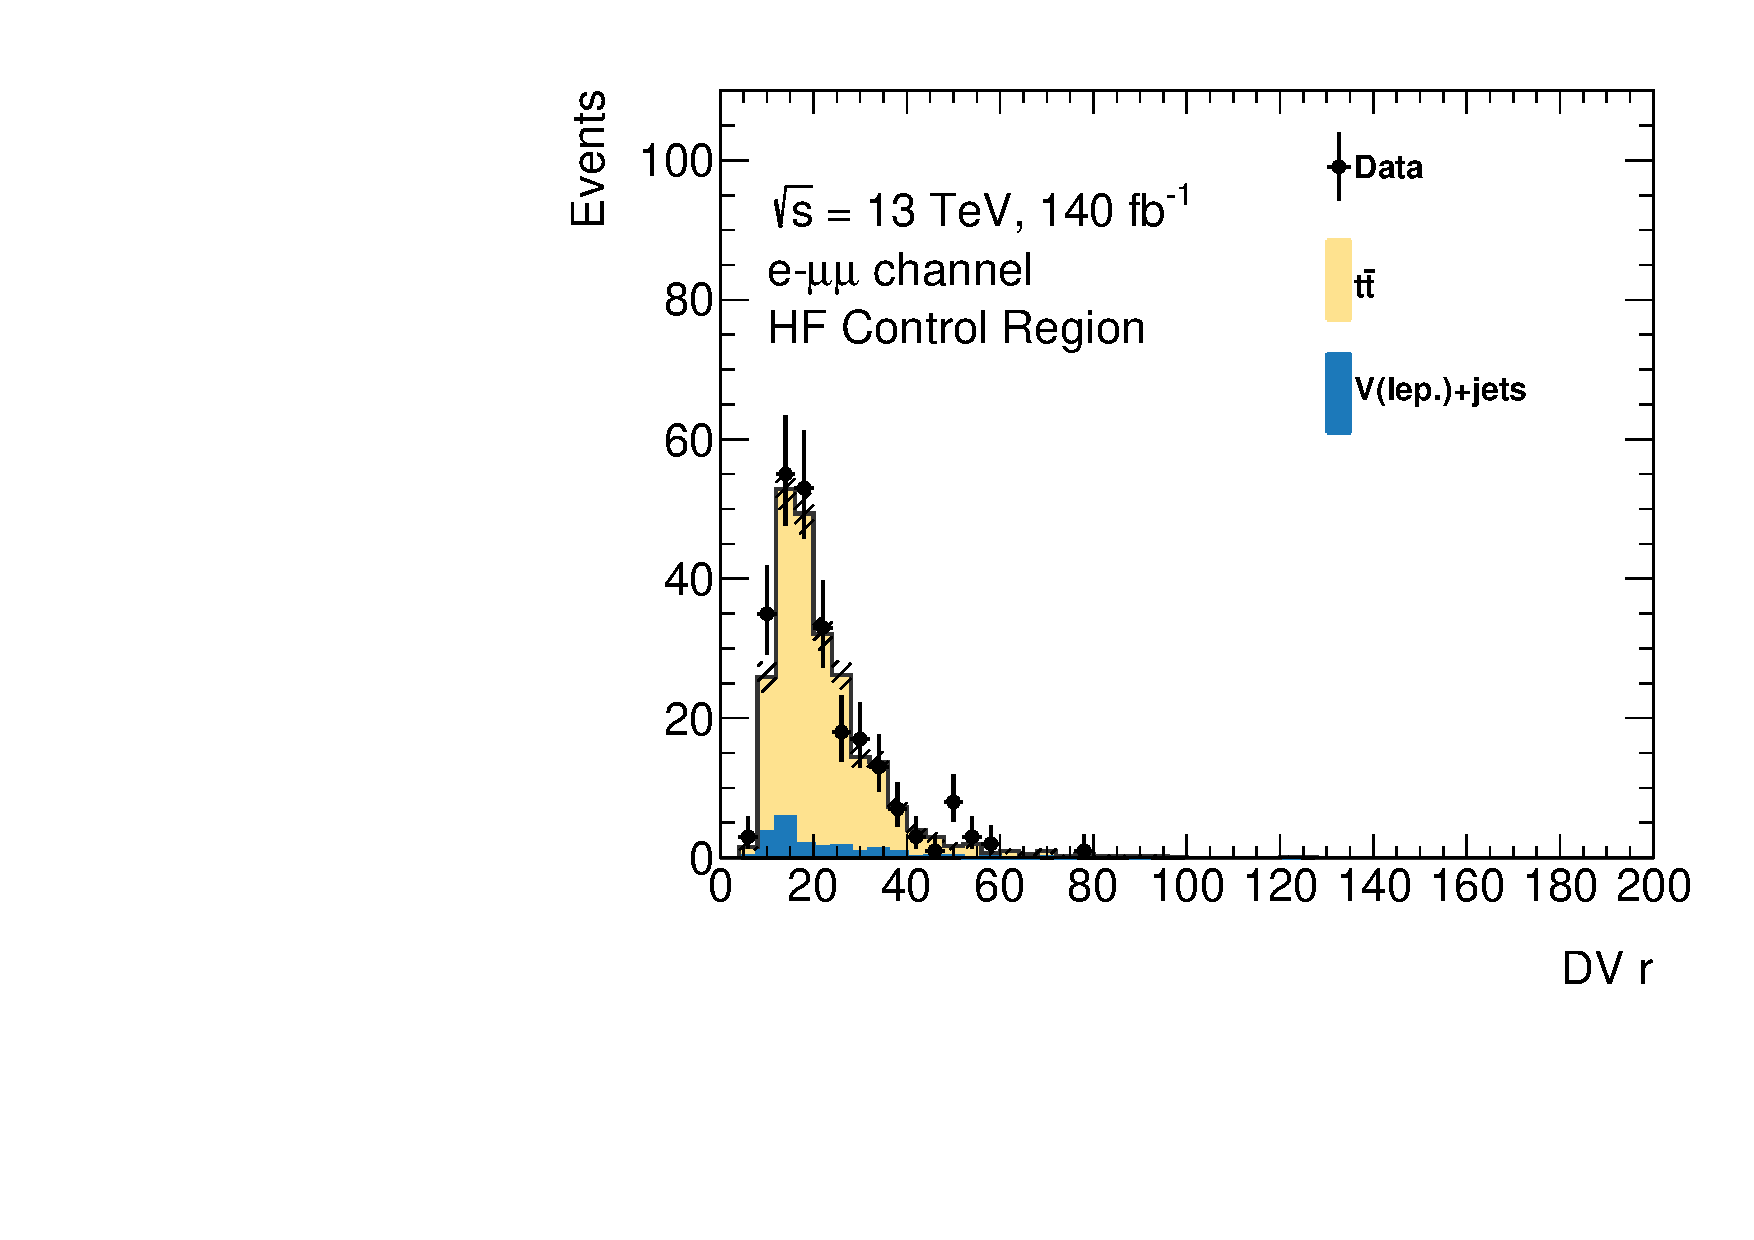
\includegraphics[width=0.24\linewidth]{figures/analysis_strategy/CR_plots/euu/DV_r.pdf}}
    \subfloat[{$\mathcal{S}$}]{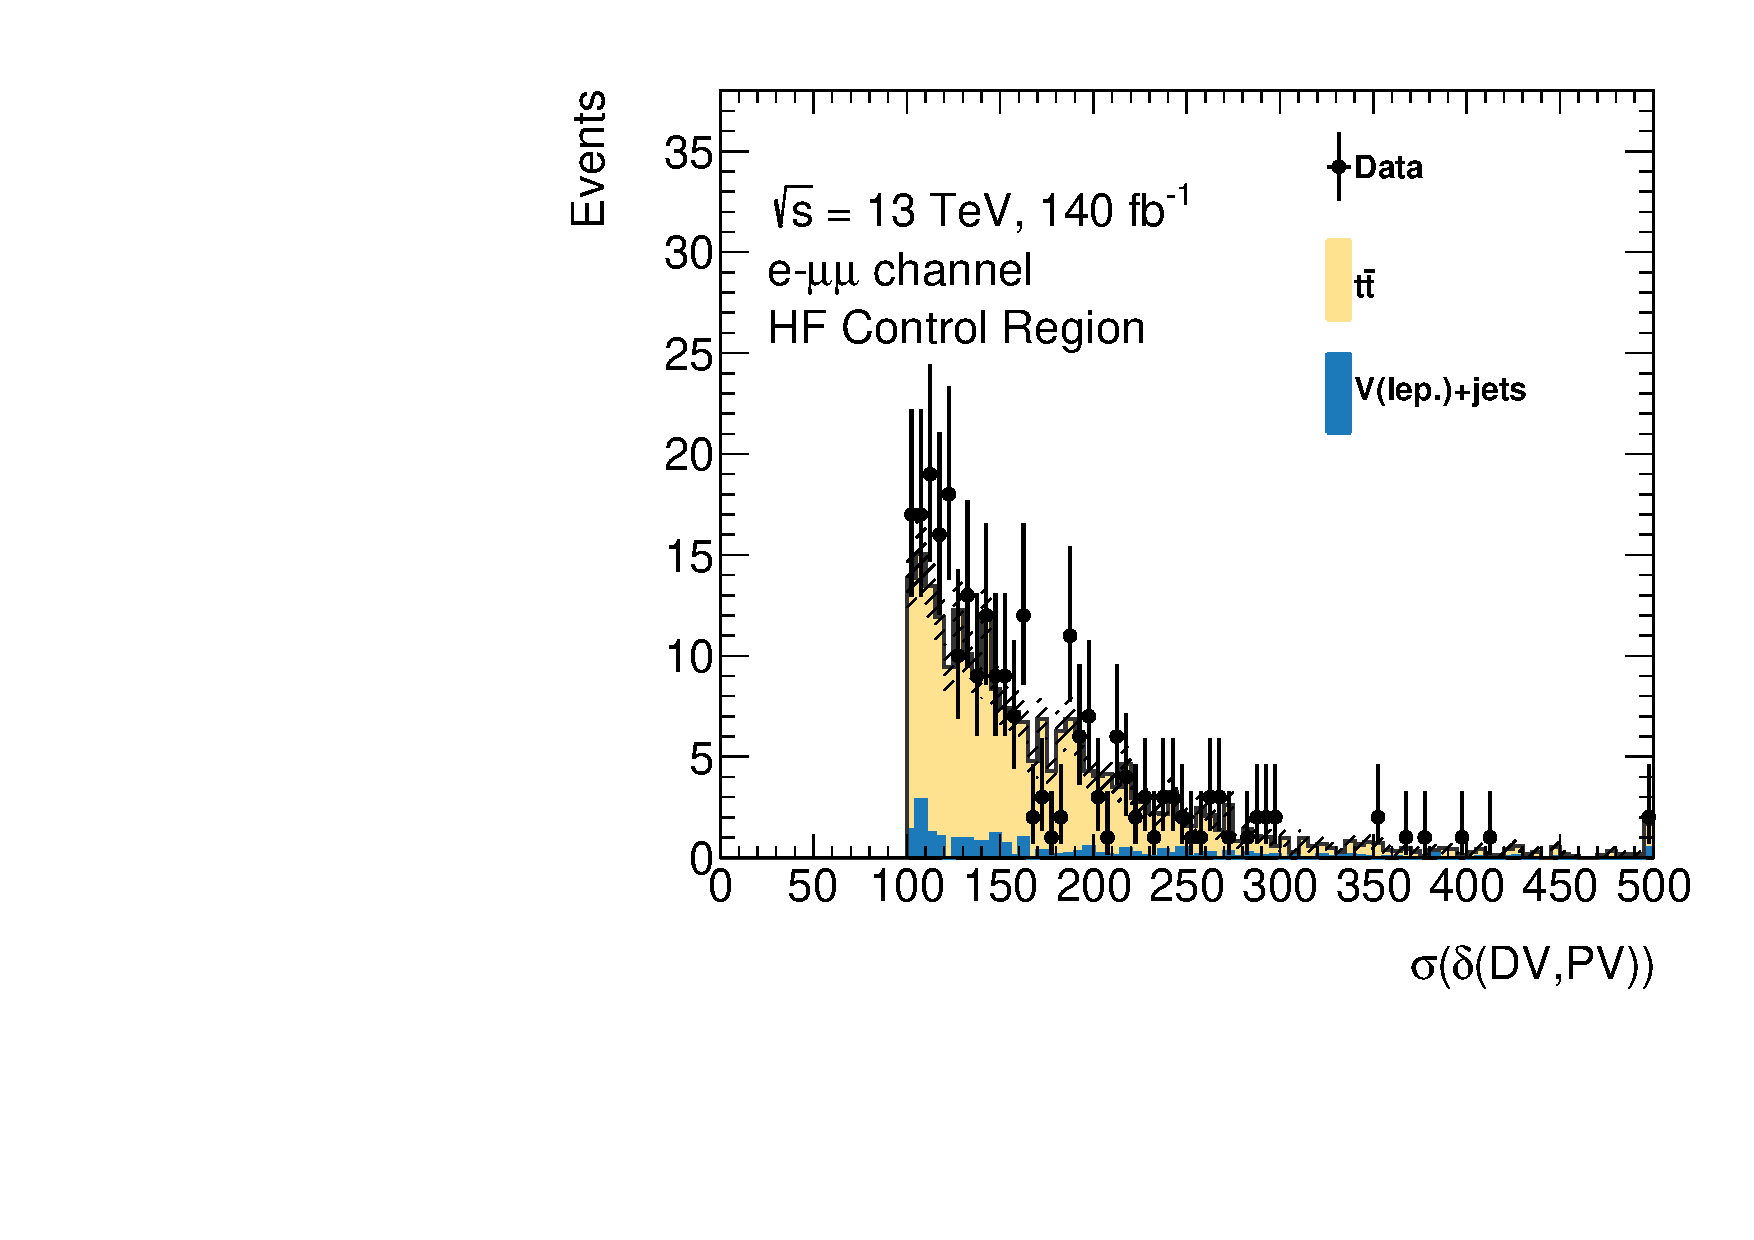
\includegraphics[width=0.24\linewidth]{figures/analysis_strategy/CR_plots/euu/DV_distFromPVsigni.pdf}}
    \subfloat[{prompt lep. \pT [GeV]}]{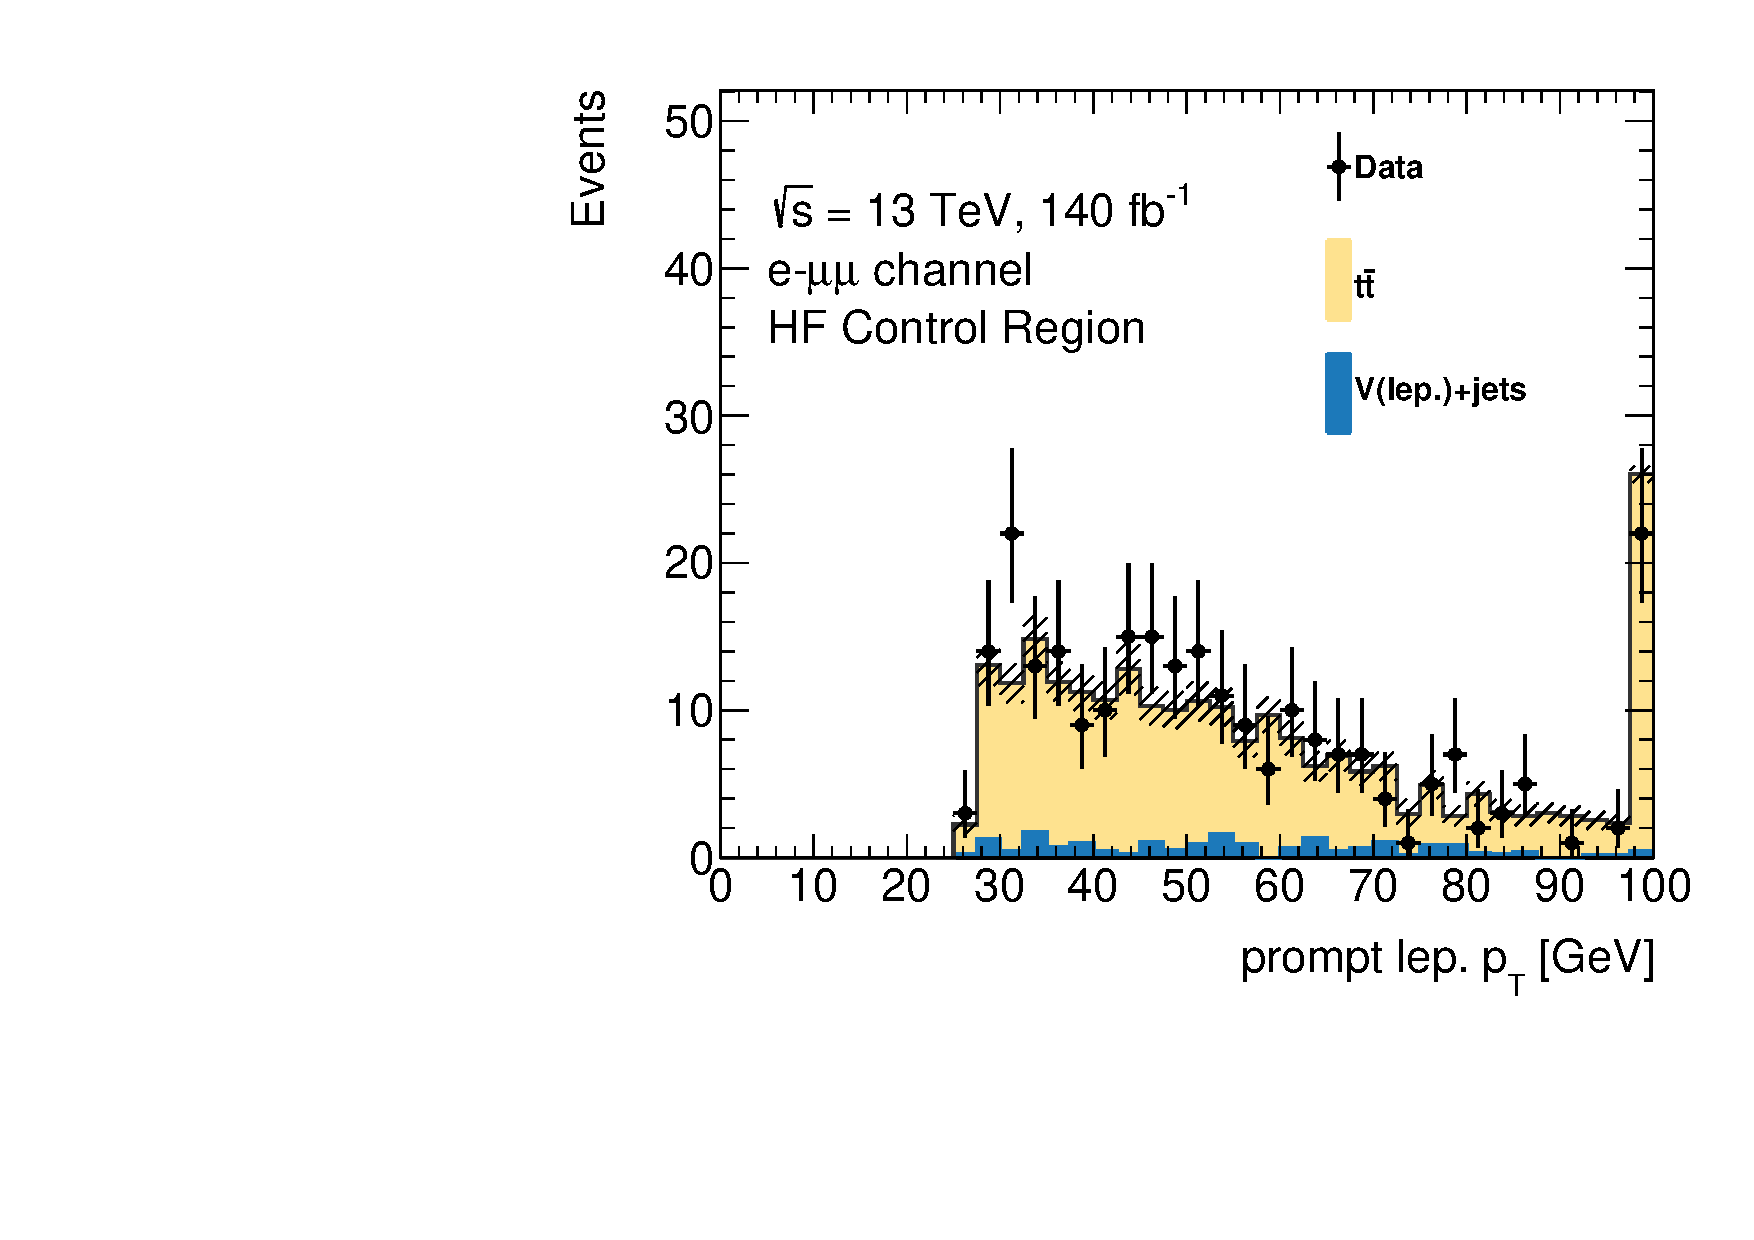
\includegraphics[width=0.24\linewidth]{figures/analysis_strategy/CR_plots/euu/prompt_lepton_pt.pdf}}\\
    \subfloat[{$\Delta R$ DV tracks}]{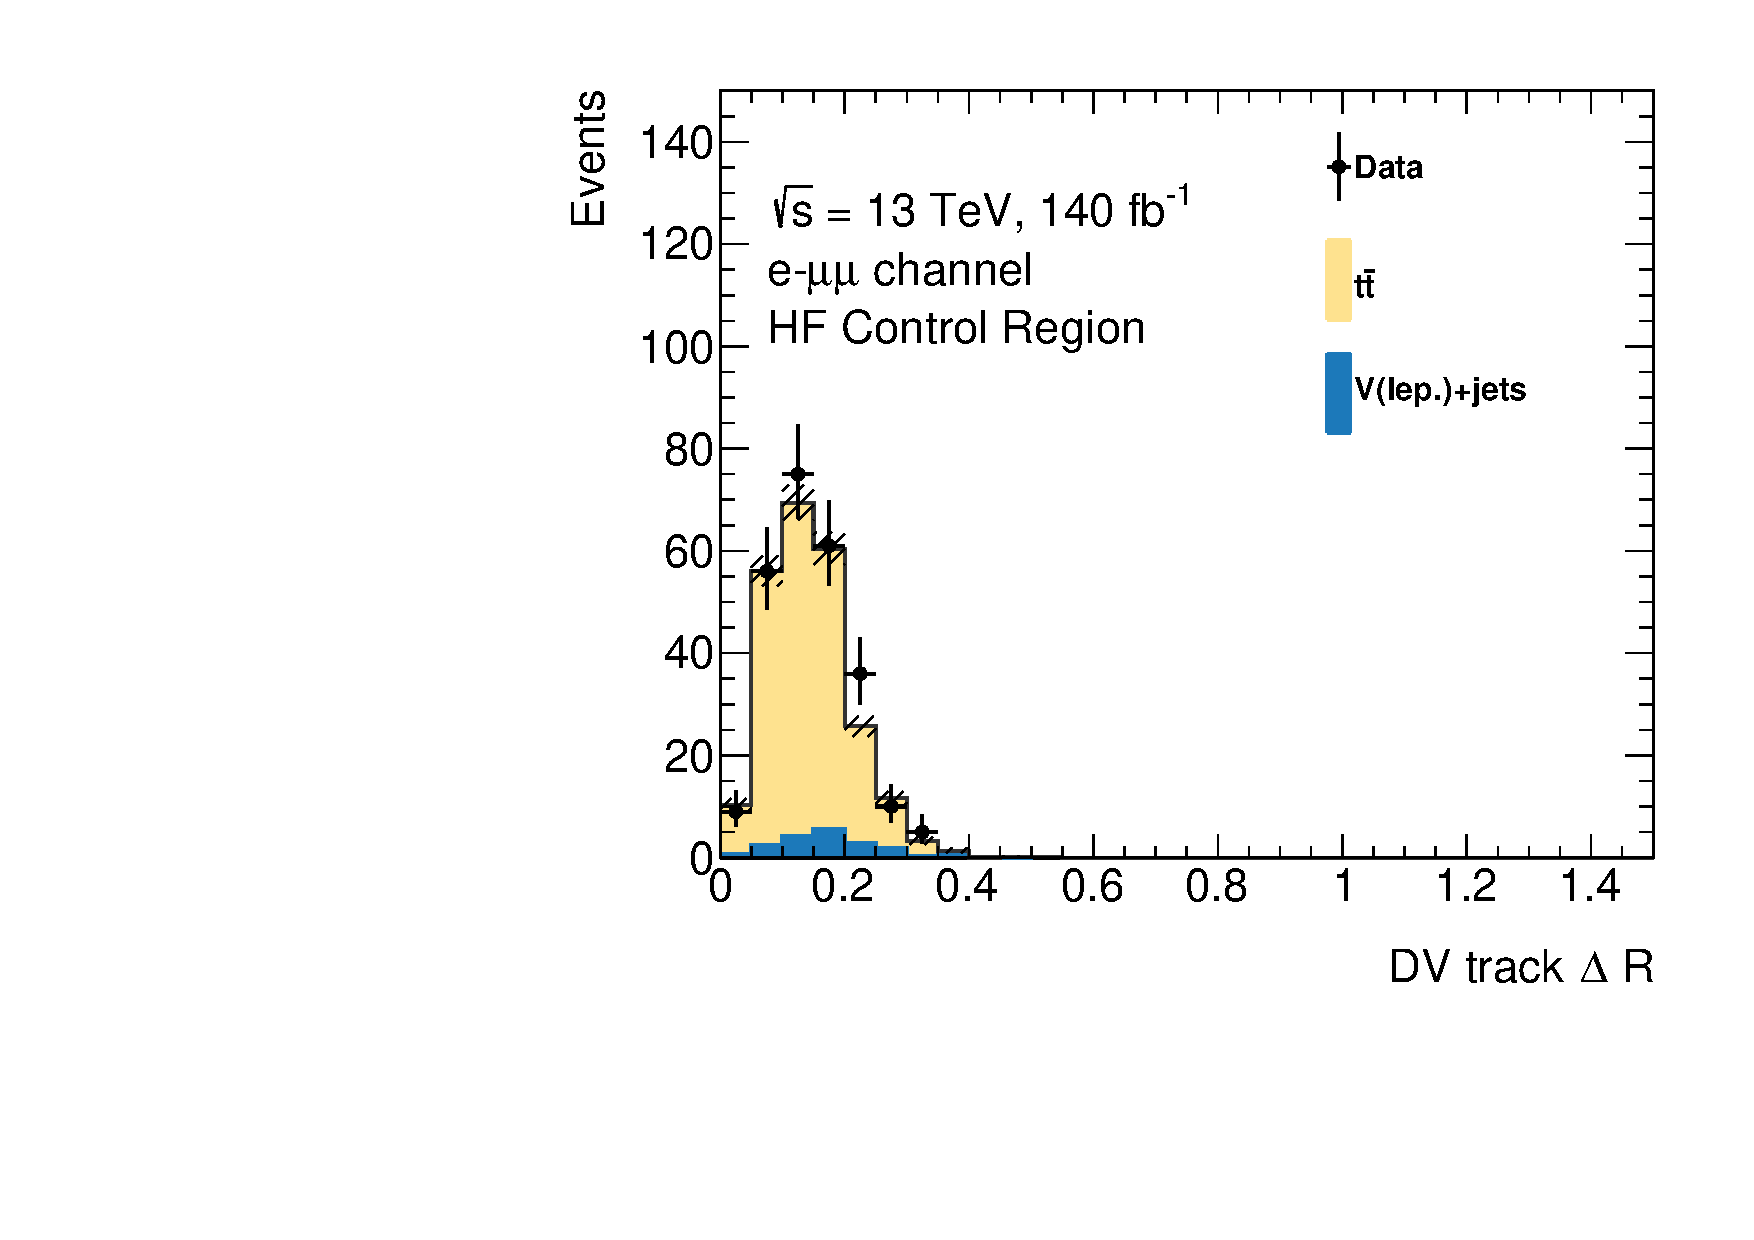
\includegraphics[width=0.24\linewidth]{figures/analysis_strategy/CR_plots/euu/DV_track_dR.pdf}}
    \subfloat[{\pT of DV tracks [GeV]}]{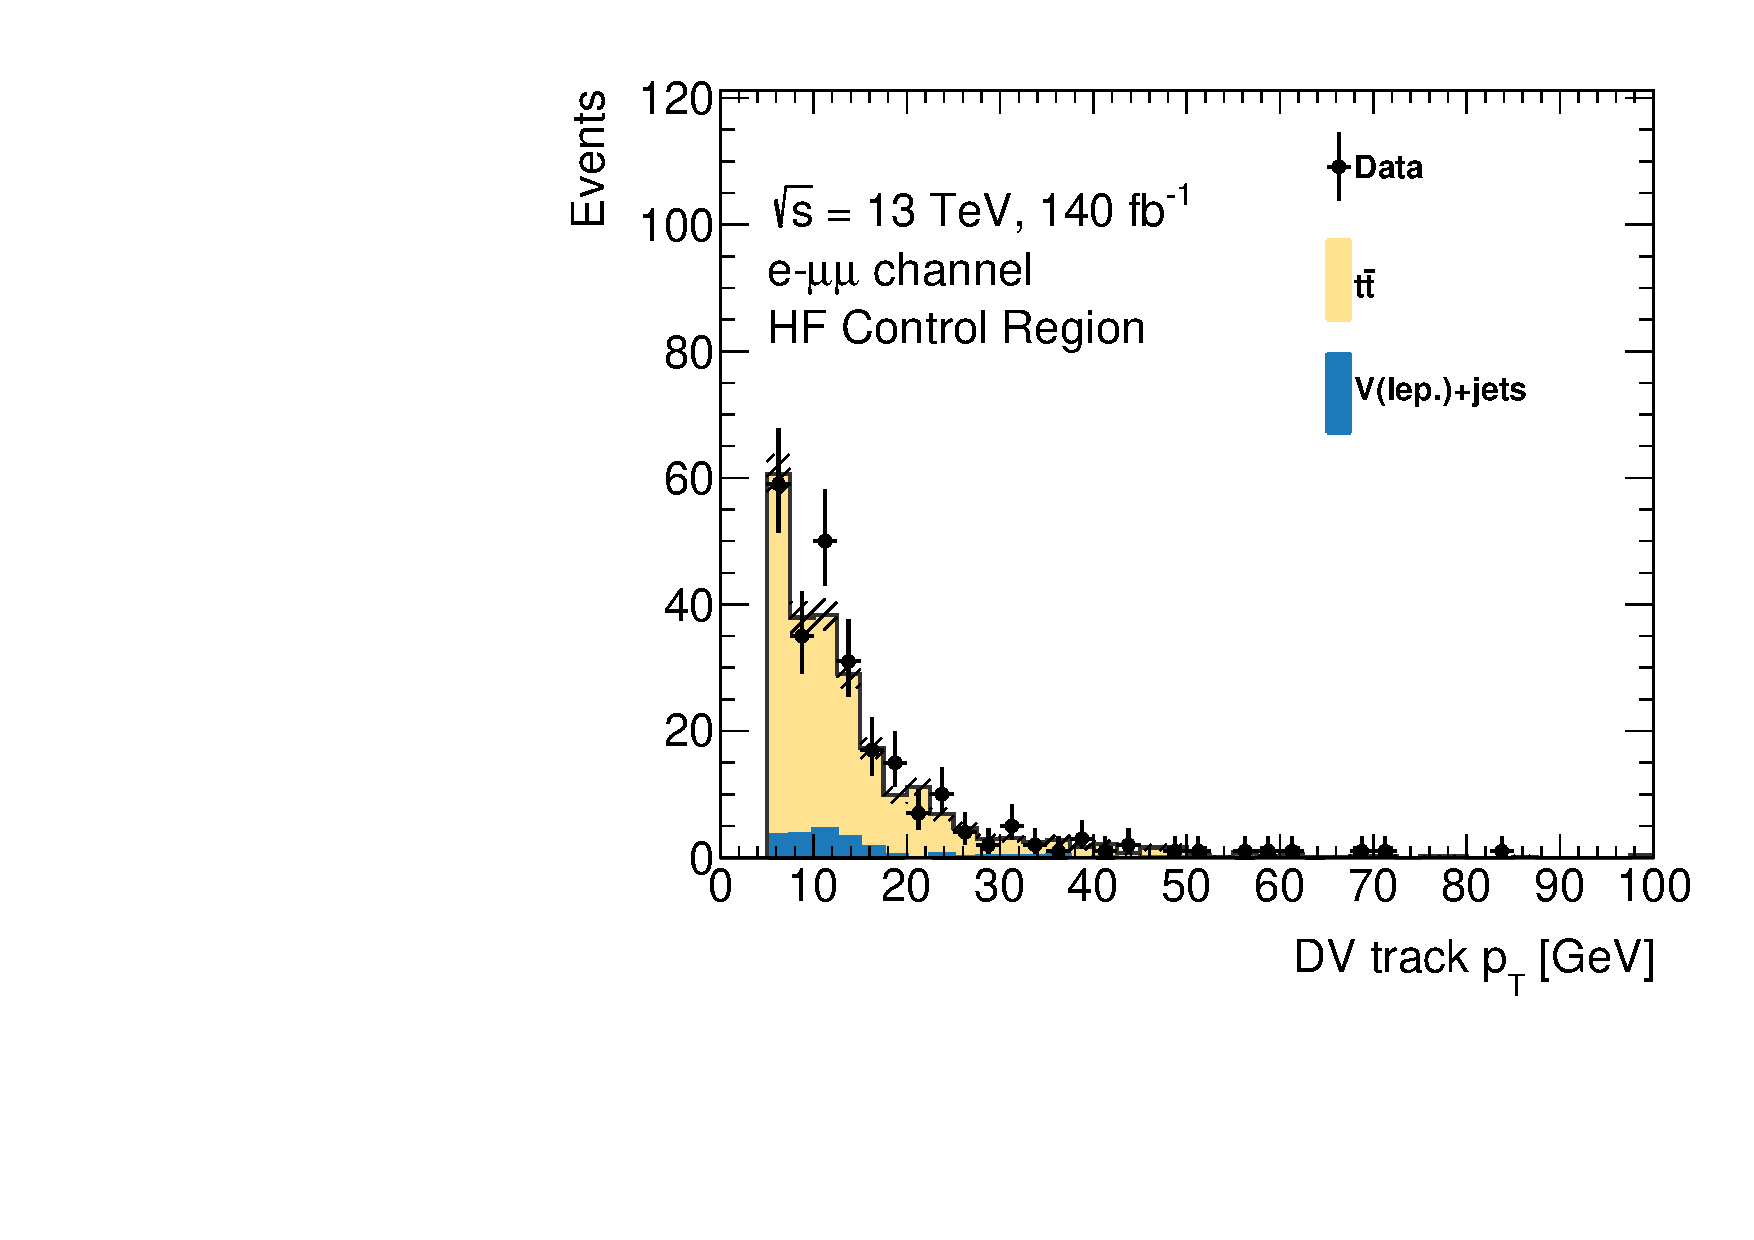
\includegraphics[width=0.24\linewidth]{figures/analysis_strategy/CR_plots/euu/DV_trk_pt.pdf}}
    \subfloat[{$\eta$ of DV tracks}]{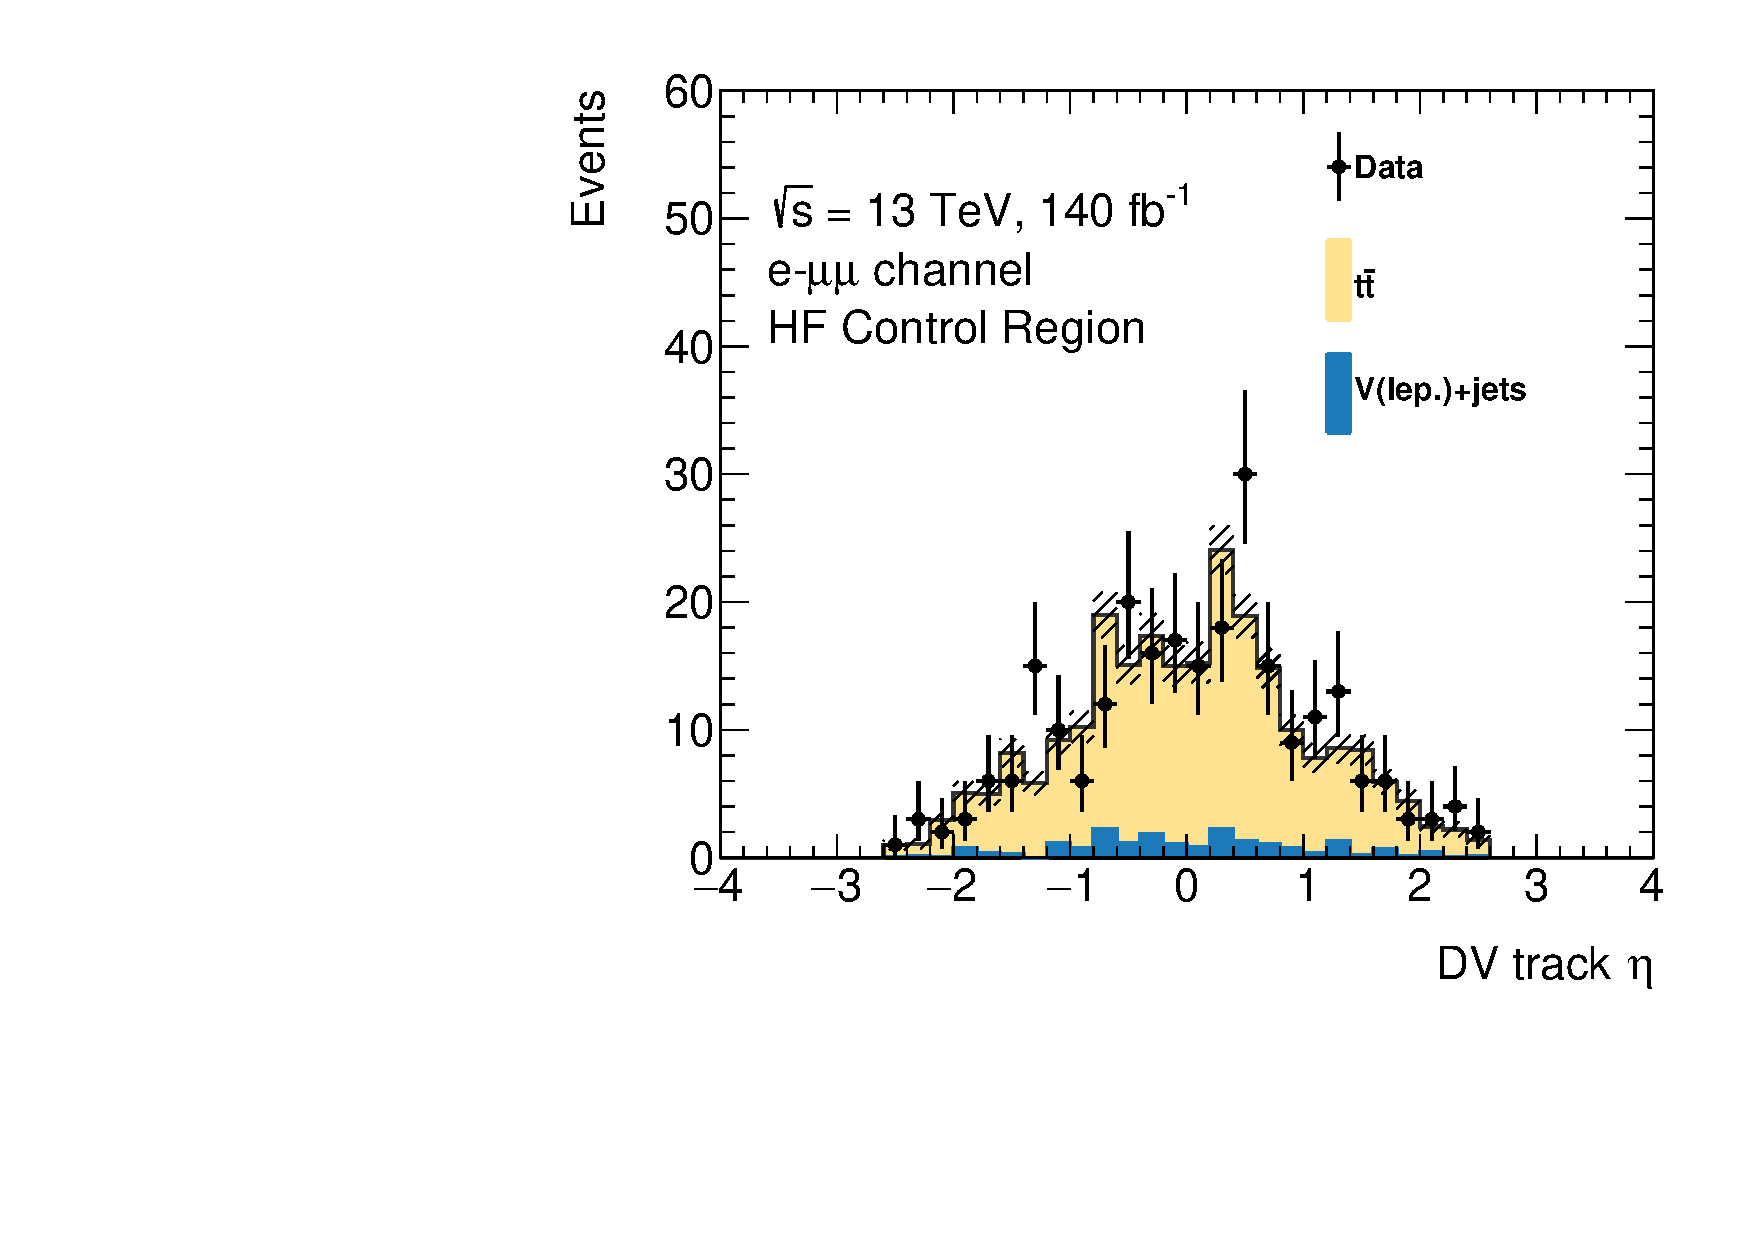
\includegraphics[width=0.24\linewidth]{figures/analysis_strategy/CR_plots/euu/DV_trk_eta.pdf}}
    \subfloat[{$d_0$ of DV tracks [mm]}]{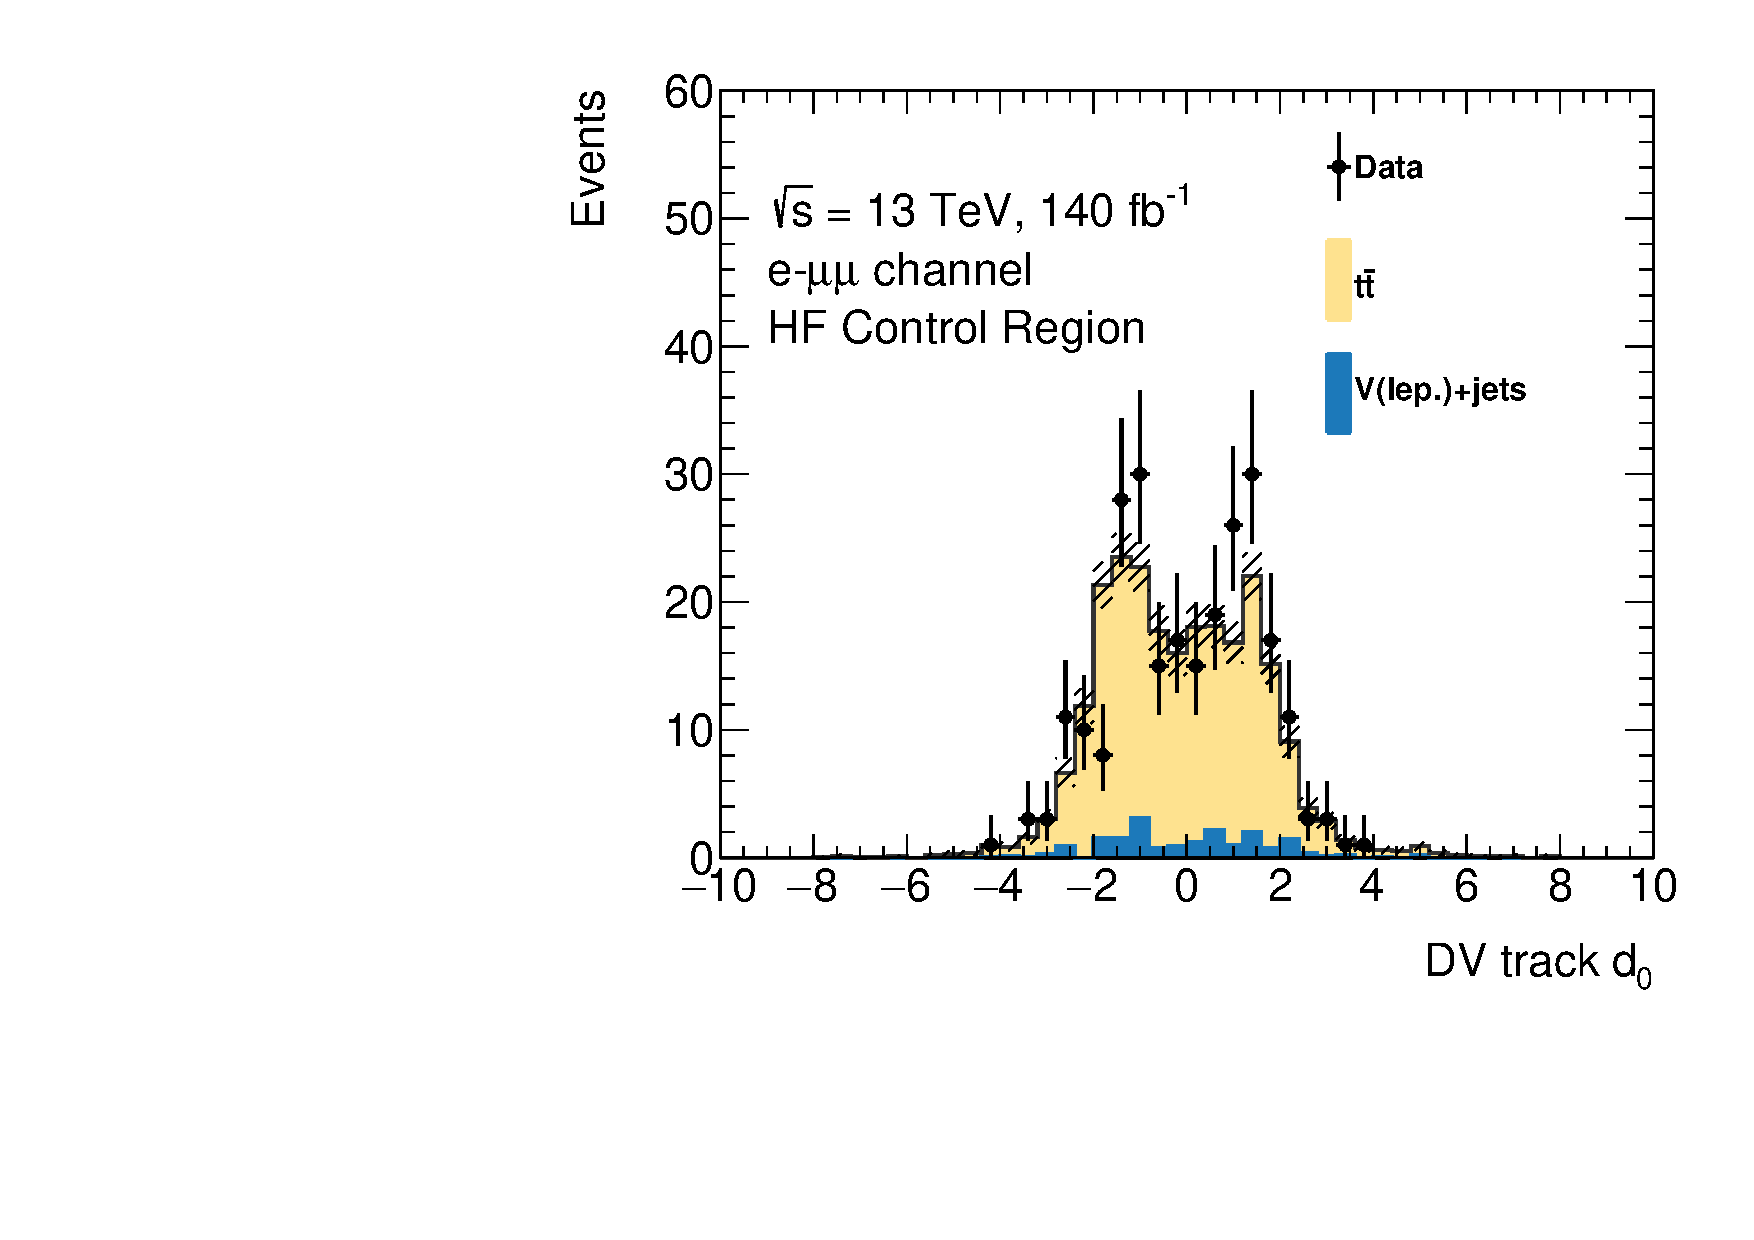
\includegraphics[width=0.24\linewidth]{figures/analysis_strategy/CR_plots/euu/DV_trk_d0.pdf}}
    \caption{Representative kinematics of the displaced vertex, tracks in the displaced vertex, and of the prompt lepton measured in ATLAS data and modeled by MC simulations in the \euu Heavy Flavor Control Region.}
    \label{fig:cr_plots_euu}
\end{figure}

\begin{figure}[!ht]
    \centering
    \subfloat[{\mdv [GeV]}]{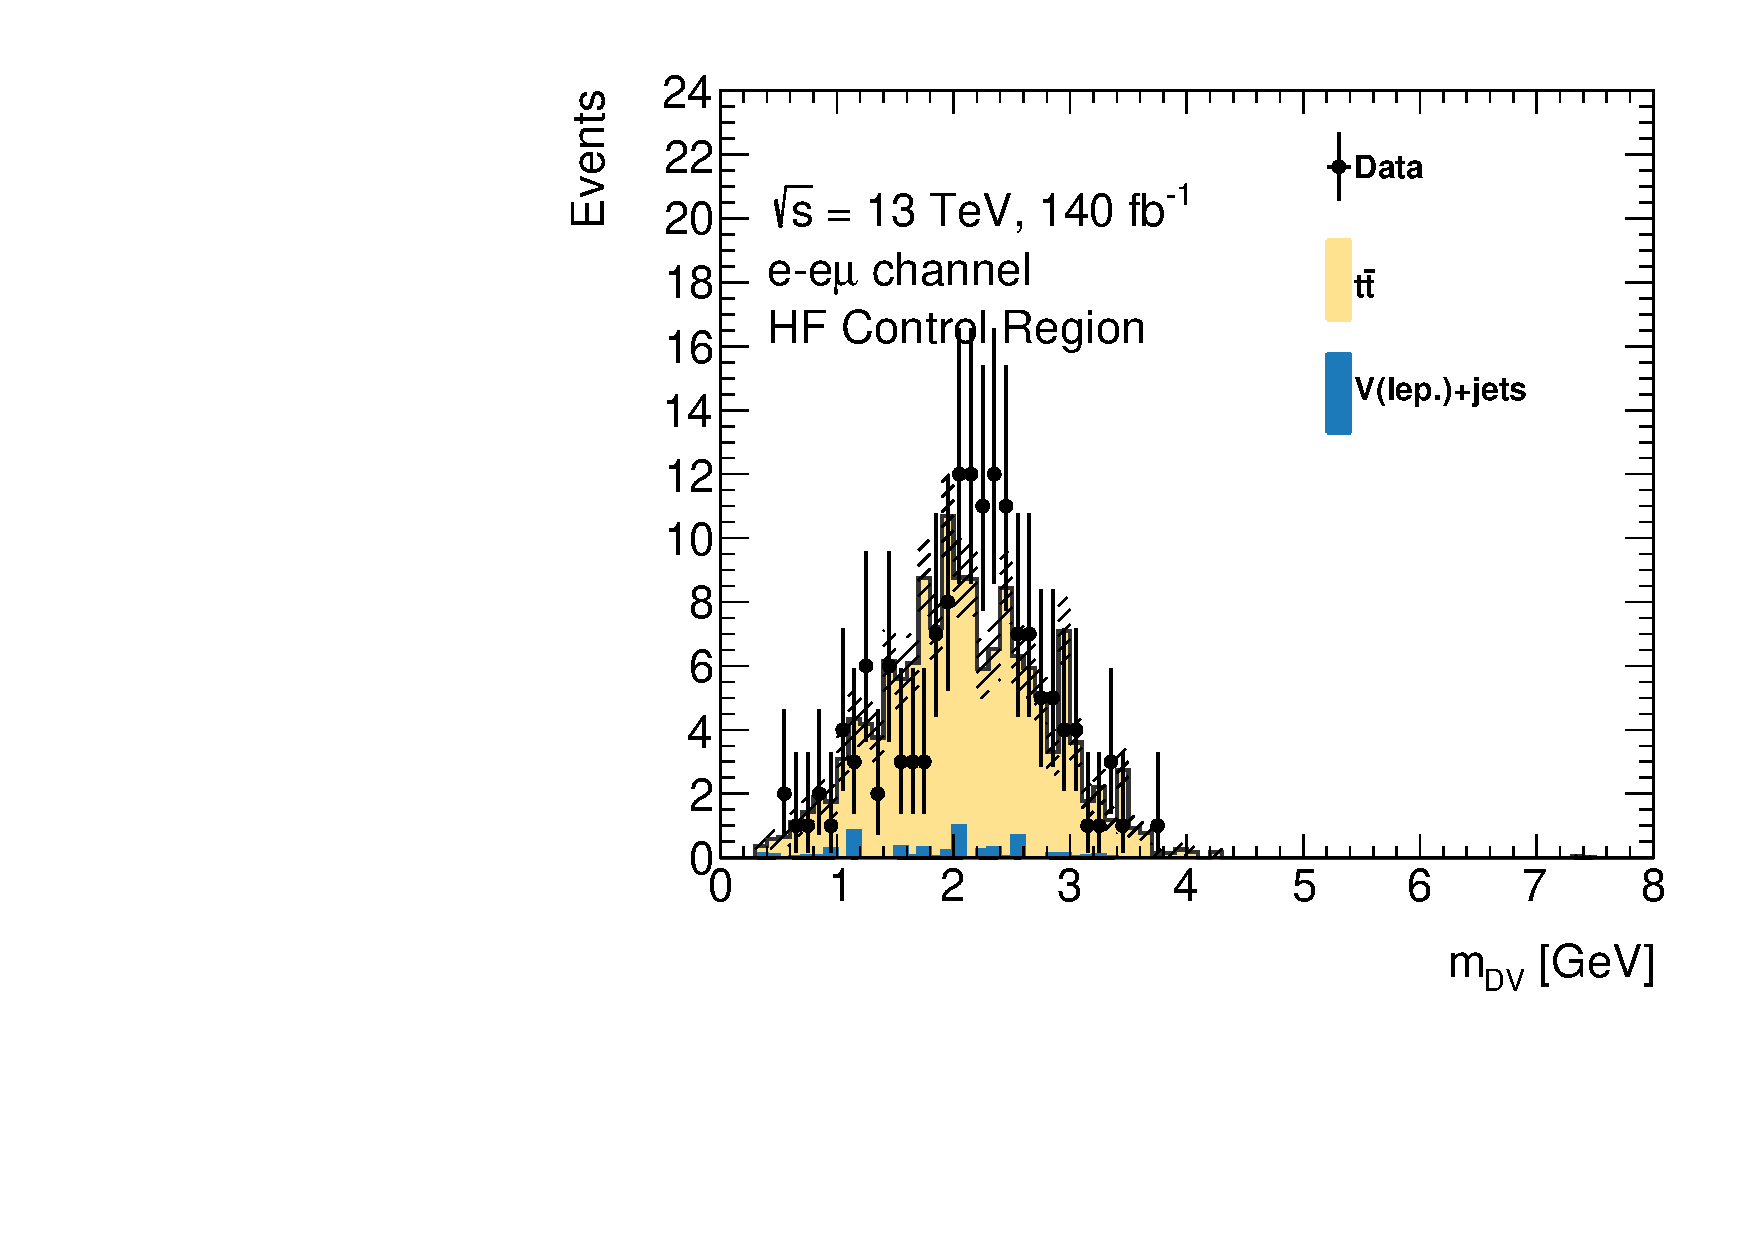
\includegraphics[width=0.24\linewidth]{figures/analysis_strategy/CR_plots/eeu/DV_mass.pdf}}
    \subfloat[{$r_\mathrm{DV}$ [mm]}]{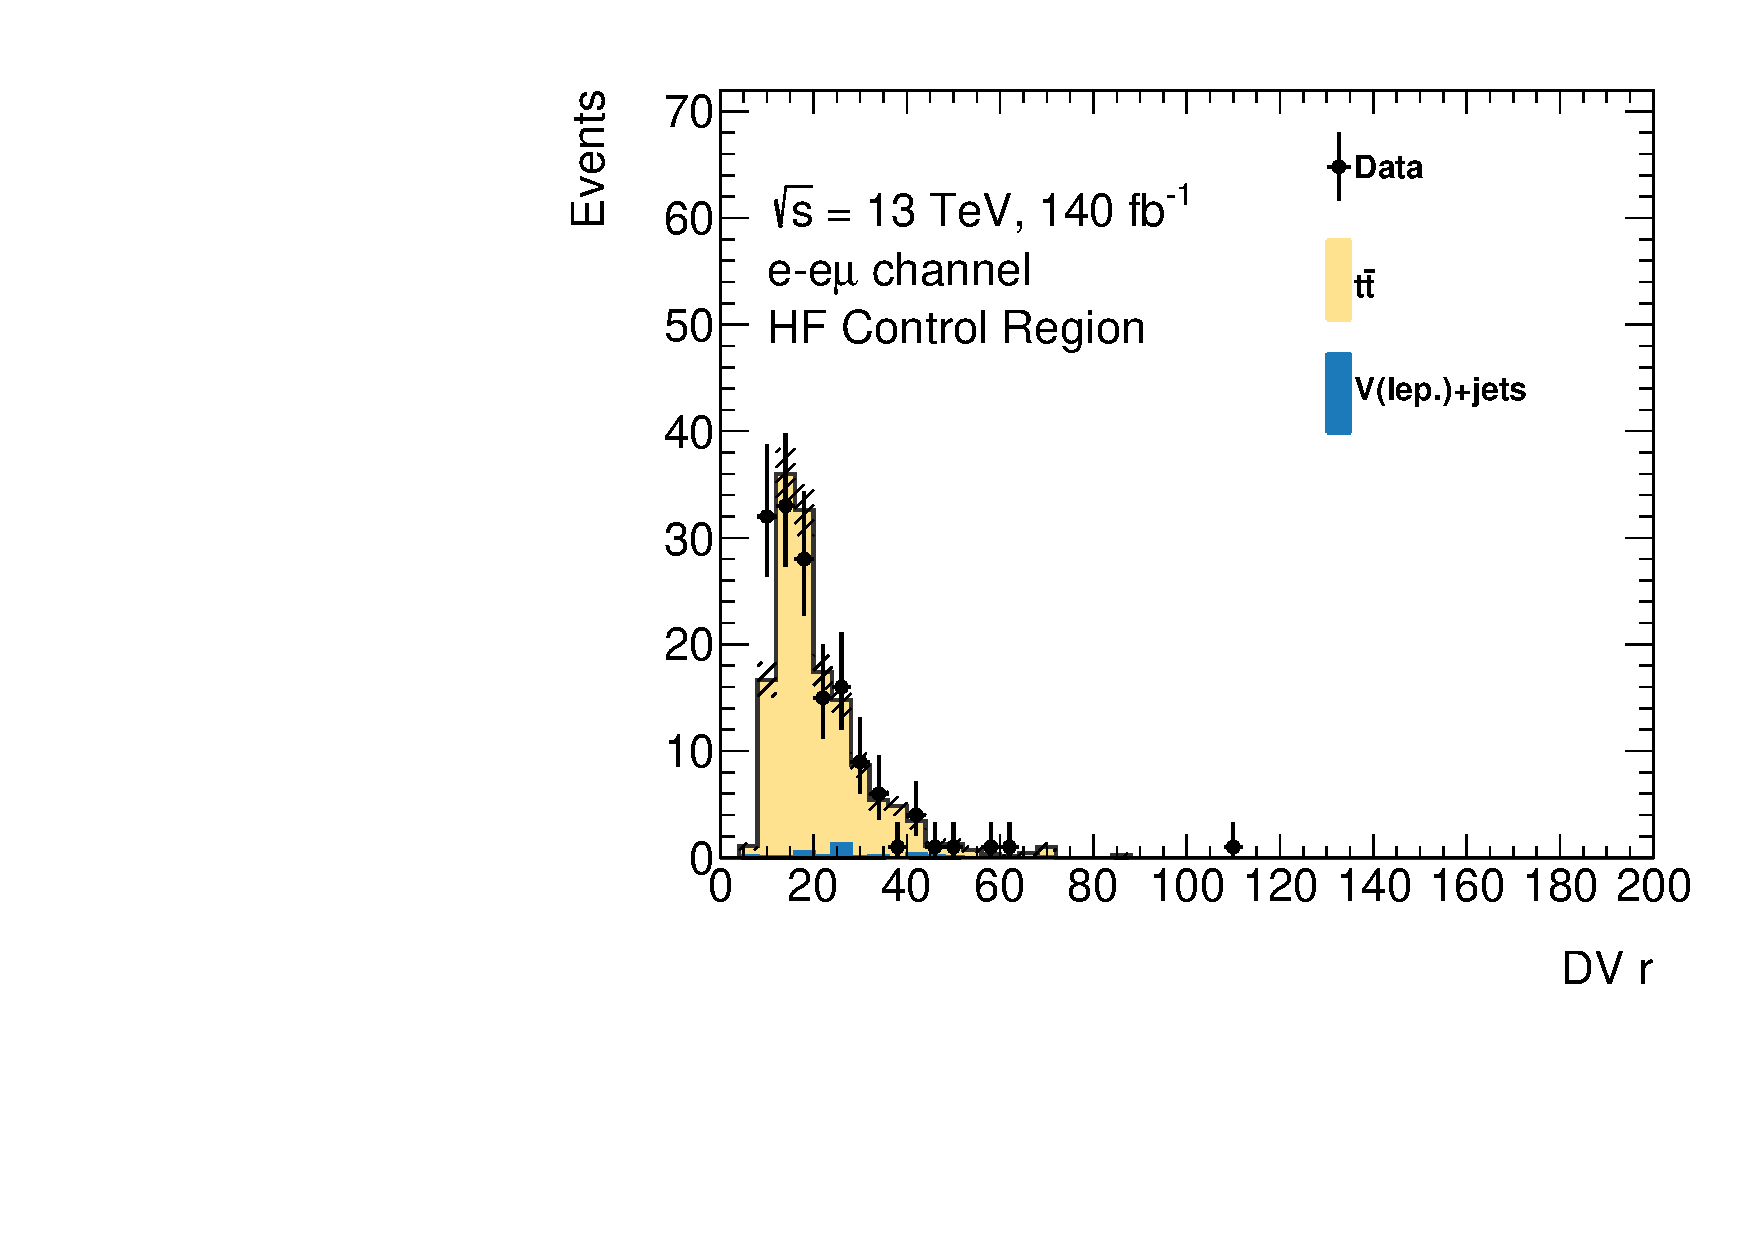
\includegraphics[width=0.24\linewidth]{figures/analysis_strategy/CR_plots/eeu/DV_r.pdf}}
    \subfloat[{$\mathcal{S}$}]{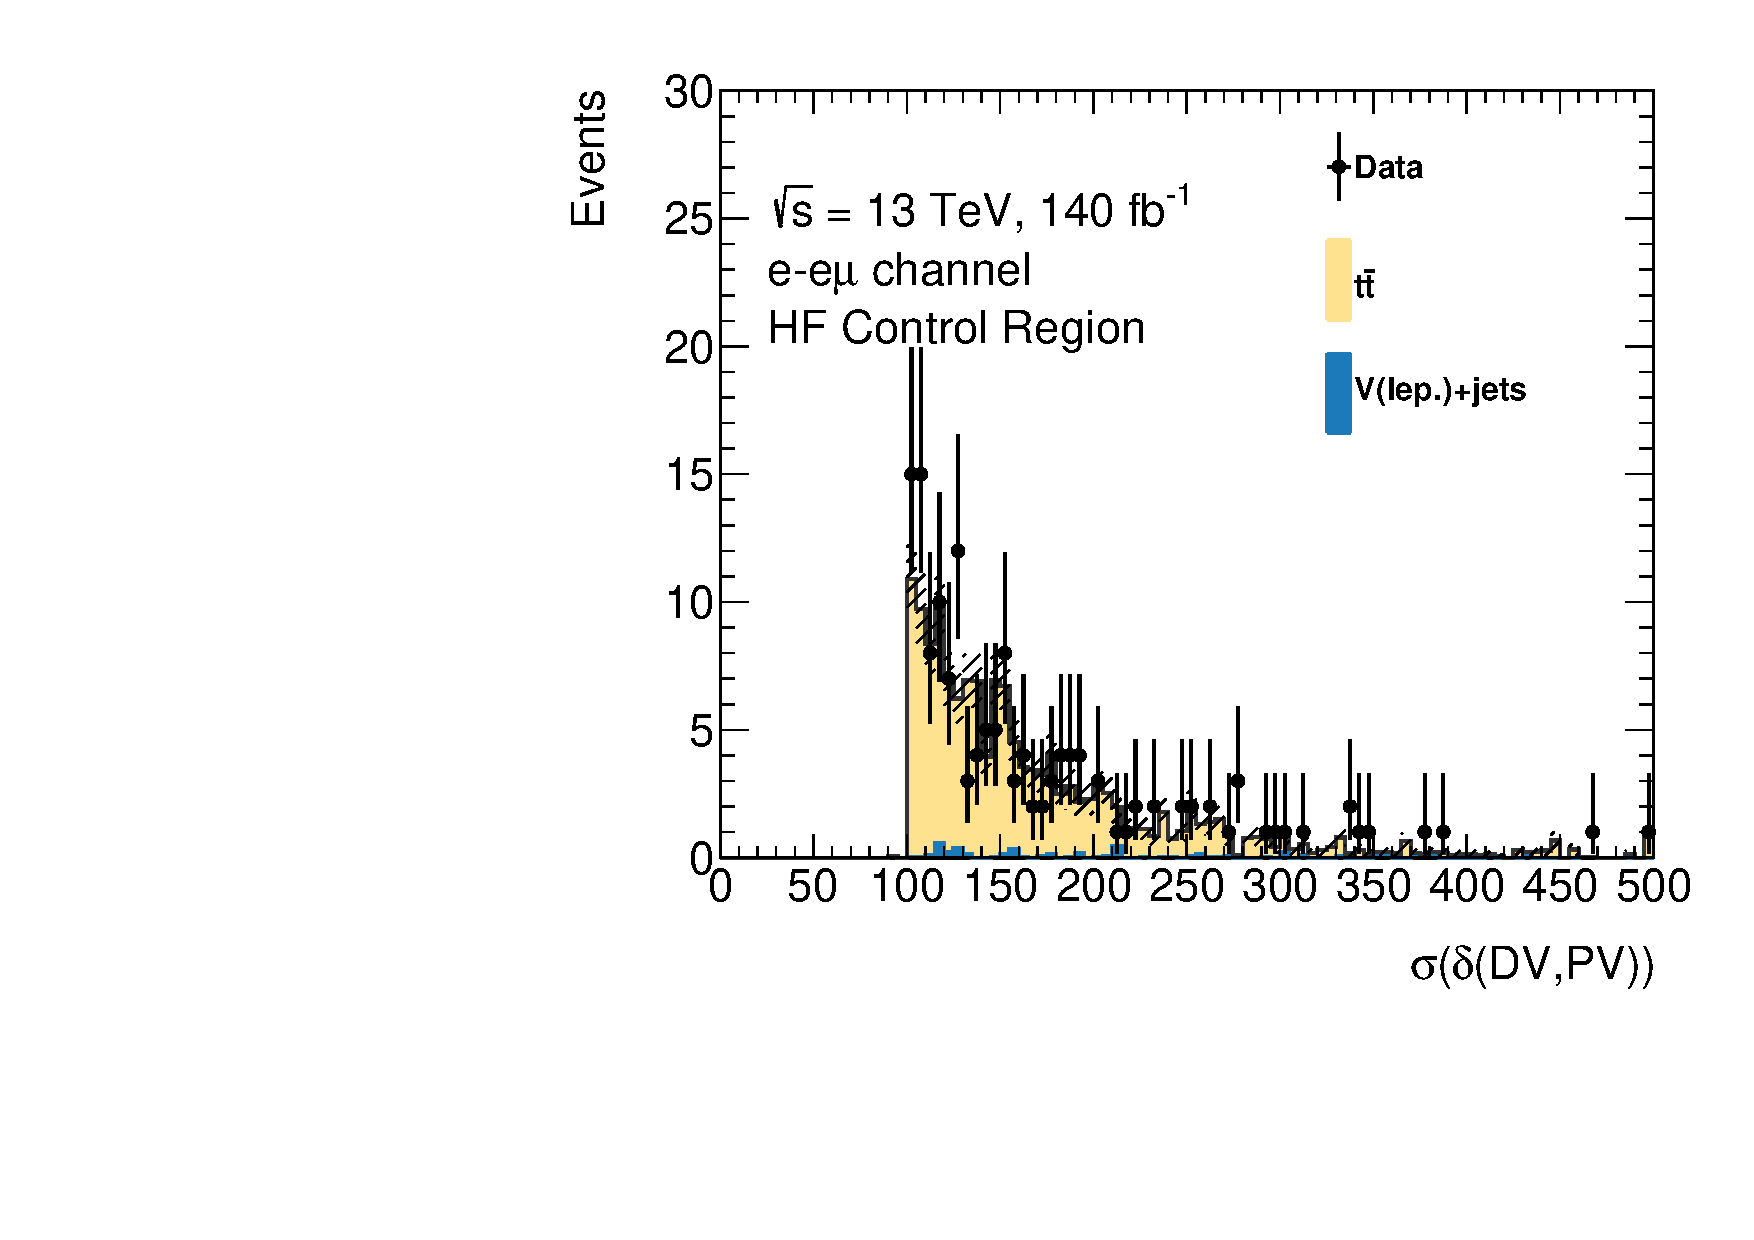
\includegraphics[width=0.24\linewidth]{figures/analysis_strategy/CR_plots/eeu/DV_distFromPVsigni.pdf}}
    \subfloat[{prompt lep. \pT [GeV]}]{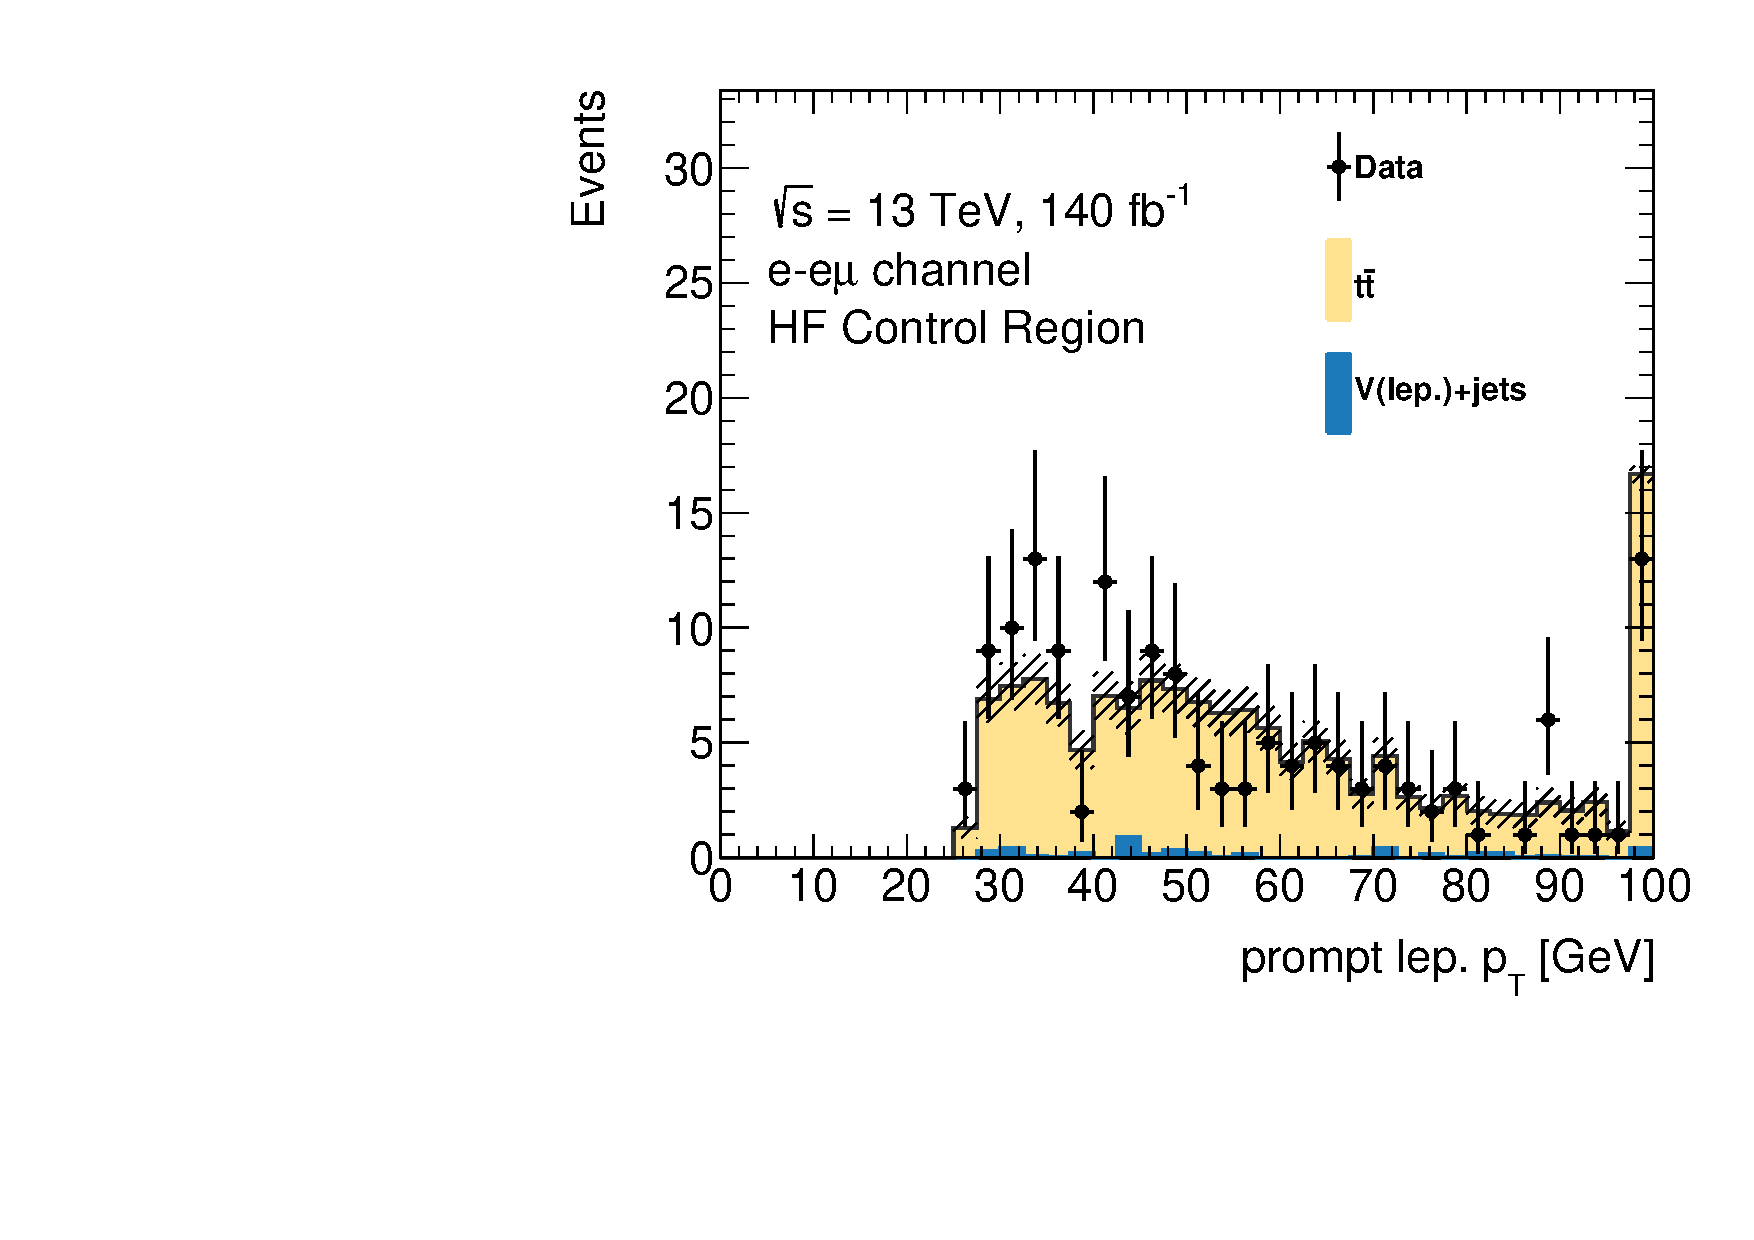
\includegraphics[width=0.24\linewidth]{figures/analysis_strategy/CR_plots/eeu/prompt_lepton_pt.pdf}}\\
    \subfloat[{$\Delta R$ DV tracks}]{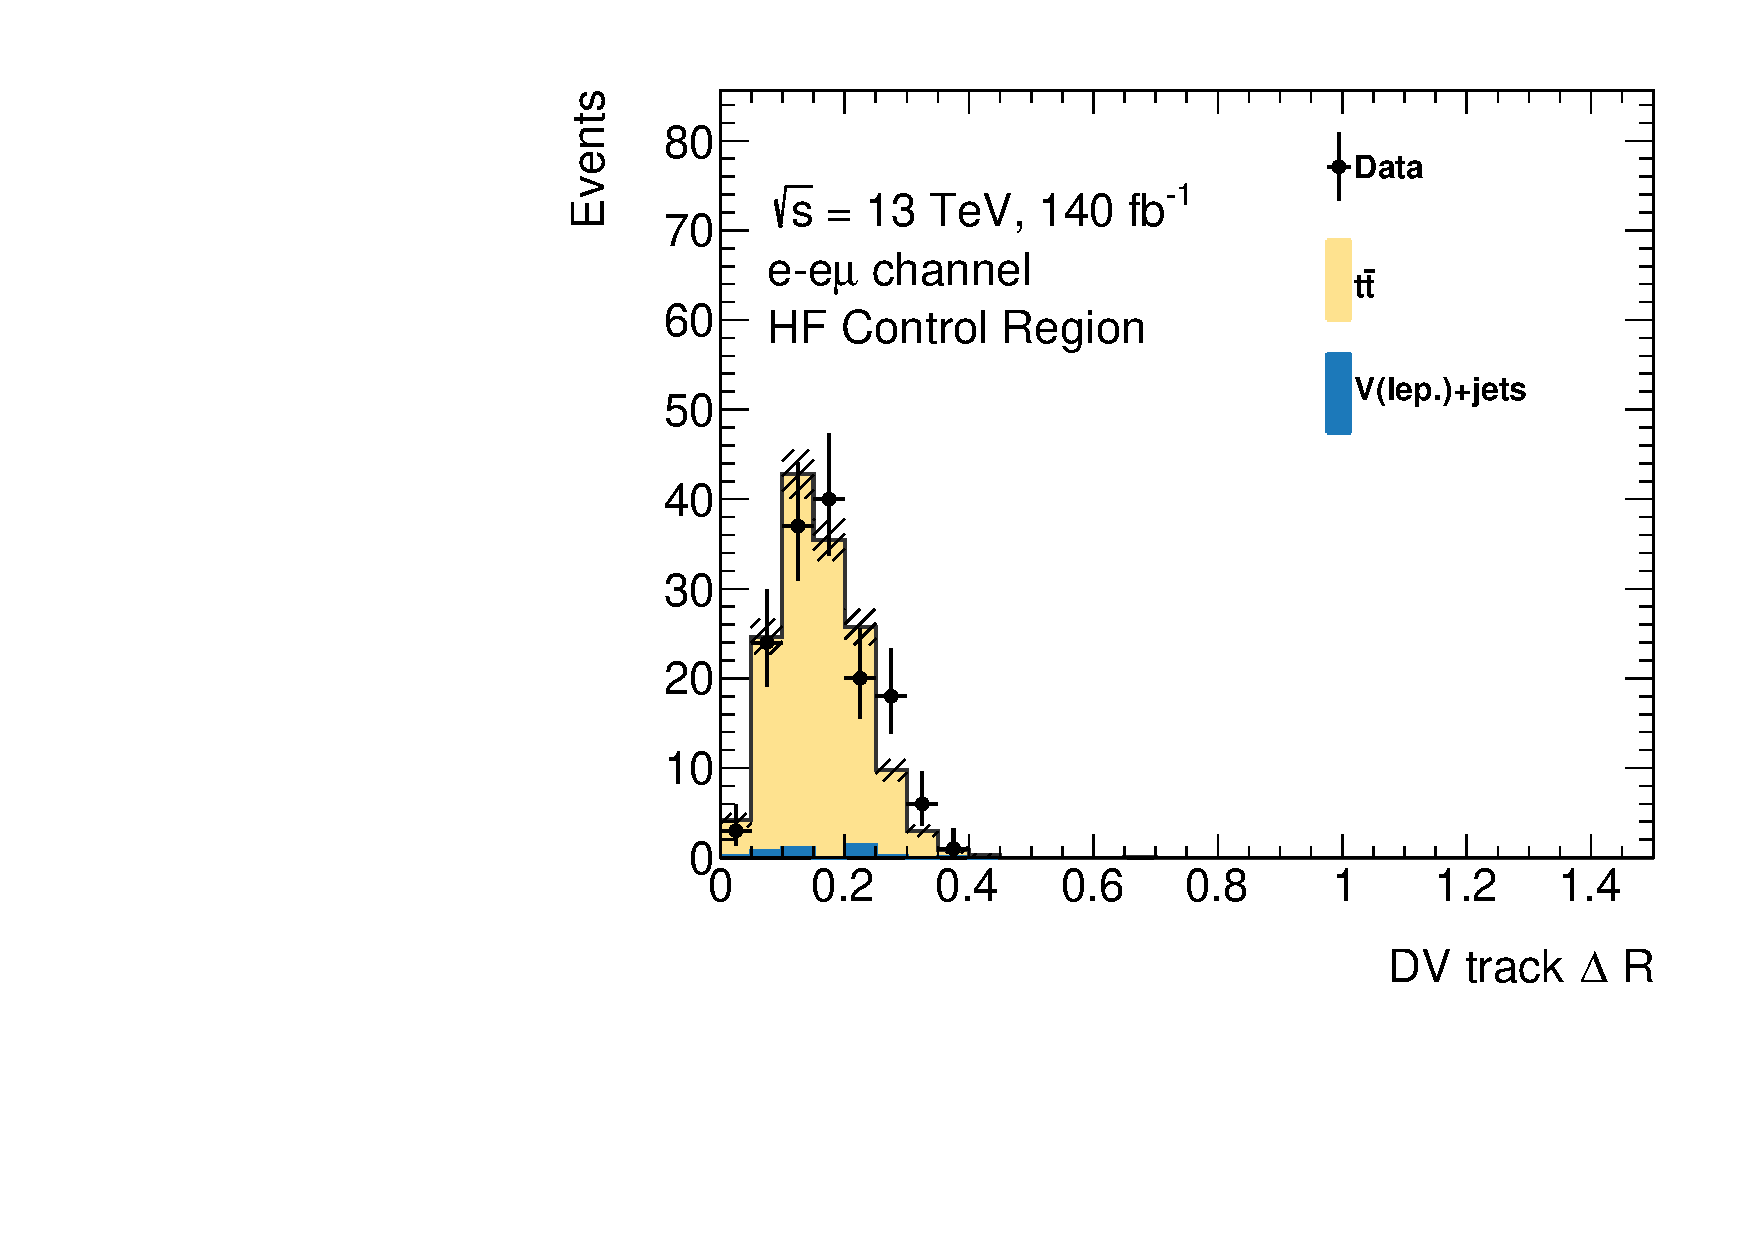
\includegraphics[width=0.24\linewidth]{figures/analysis_strategy/CR_plots/eeu/DV_track_dR.pdf}}
    \subfloat[{\pT of DV tracks [GeV]}]{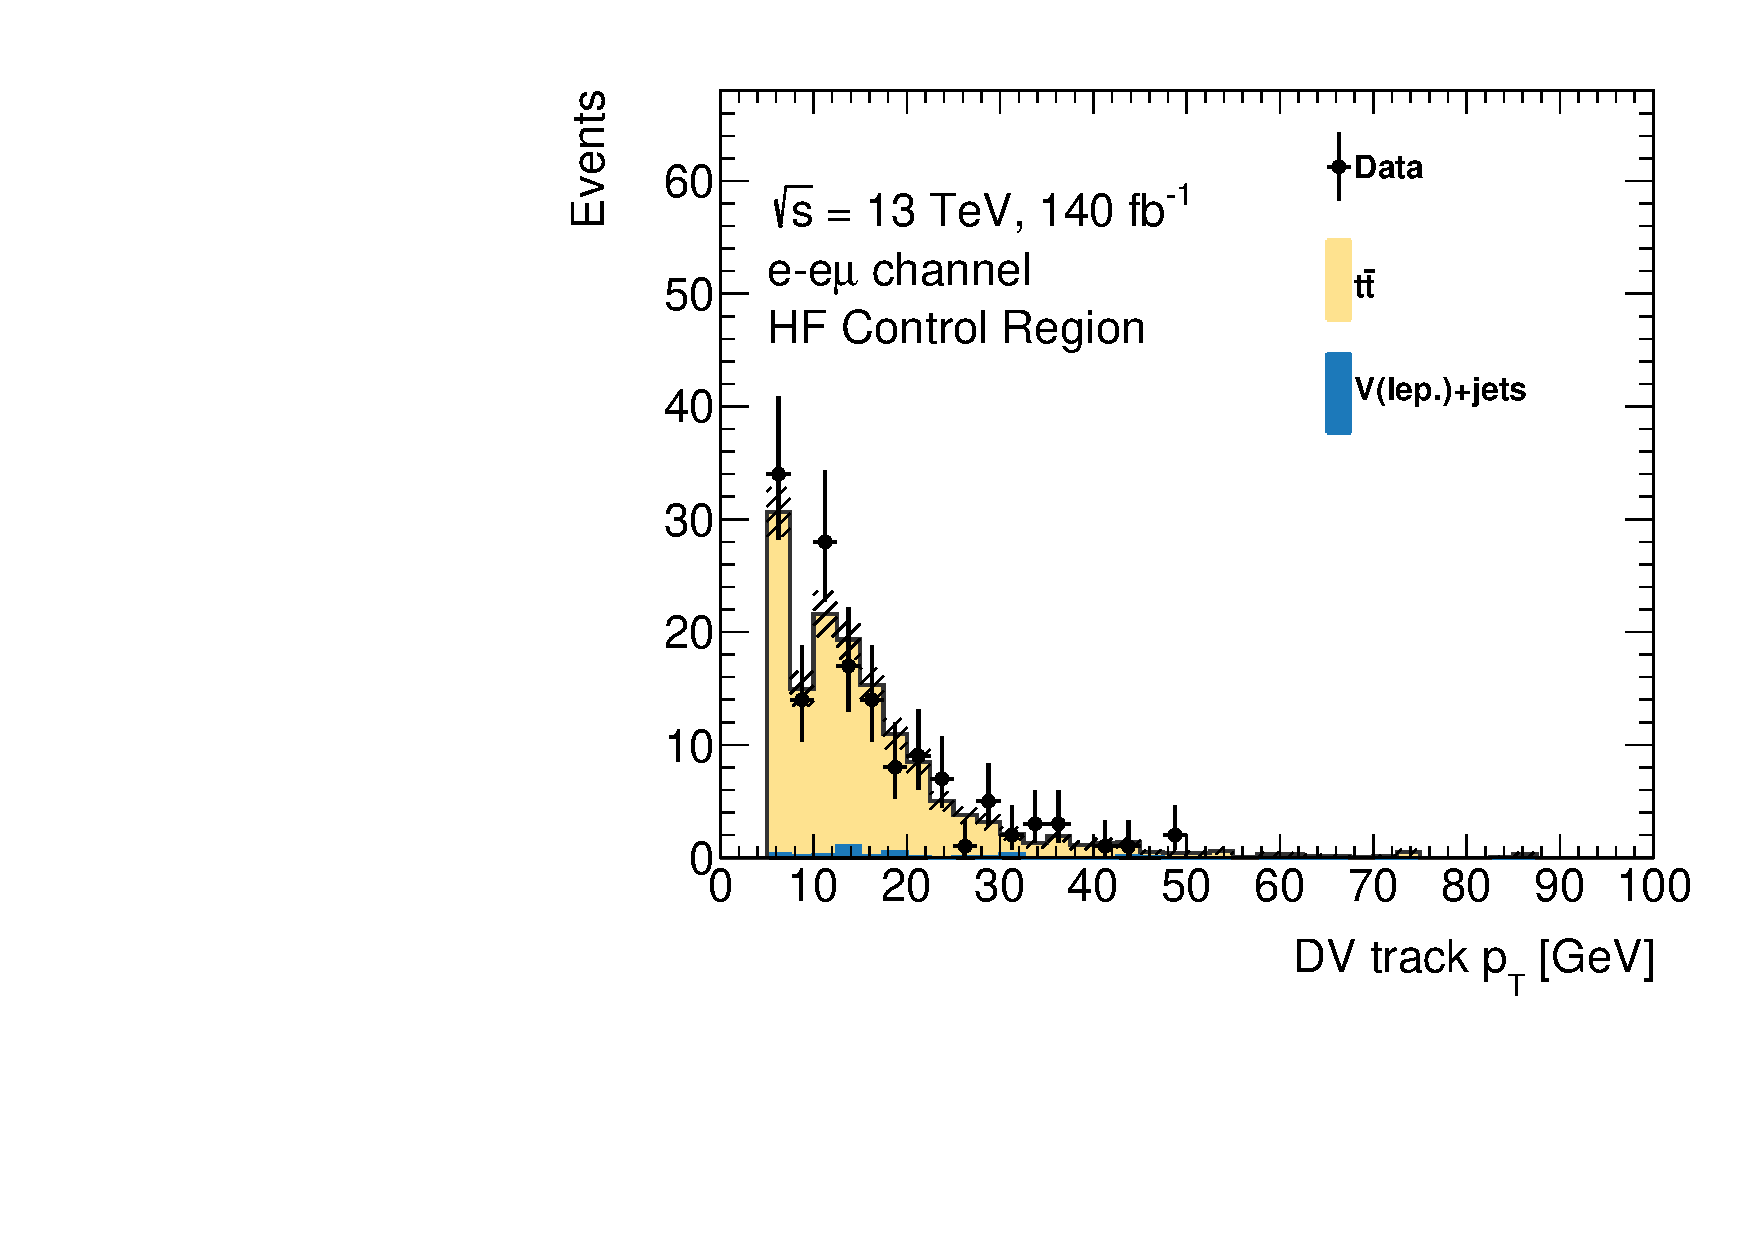
\includegraphics[width=0.24\linewidth]{figures/analysis_strategy/CR_plots/eeu/DV_trk_pt.pdf}}
    \subfloat[{$\eta$ of DV tracks}]{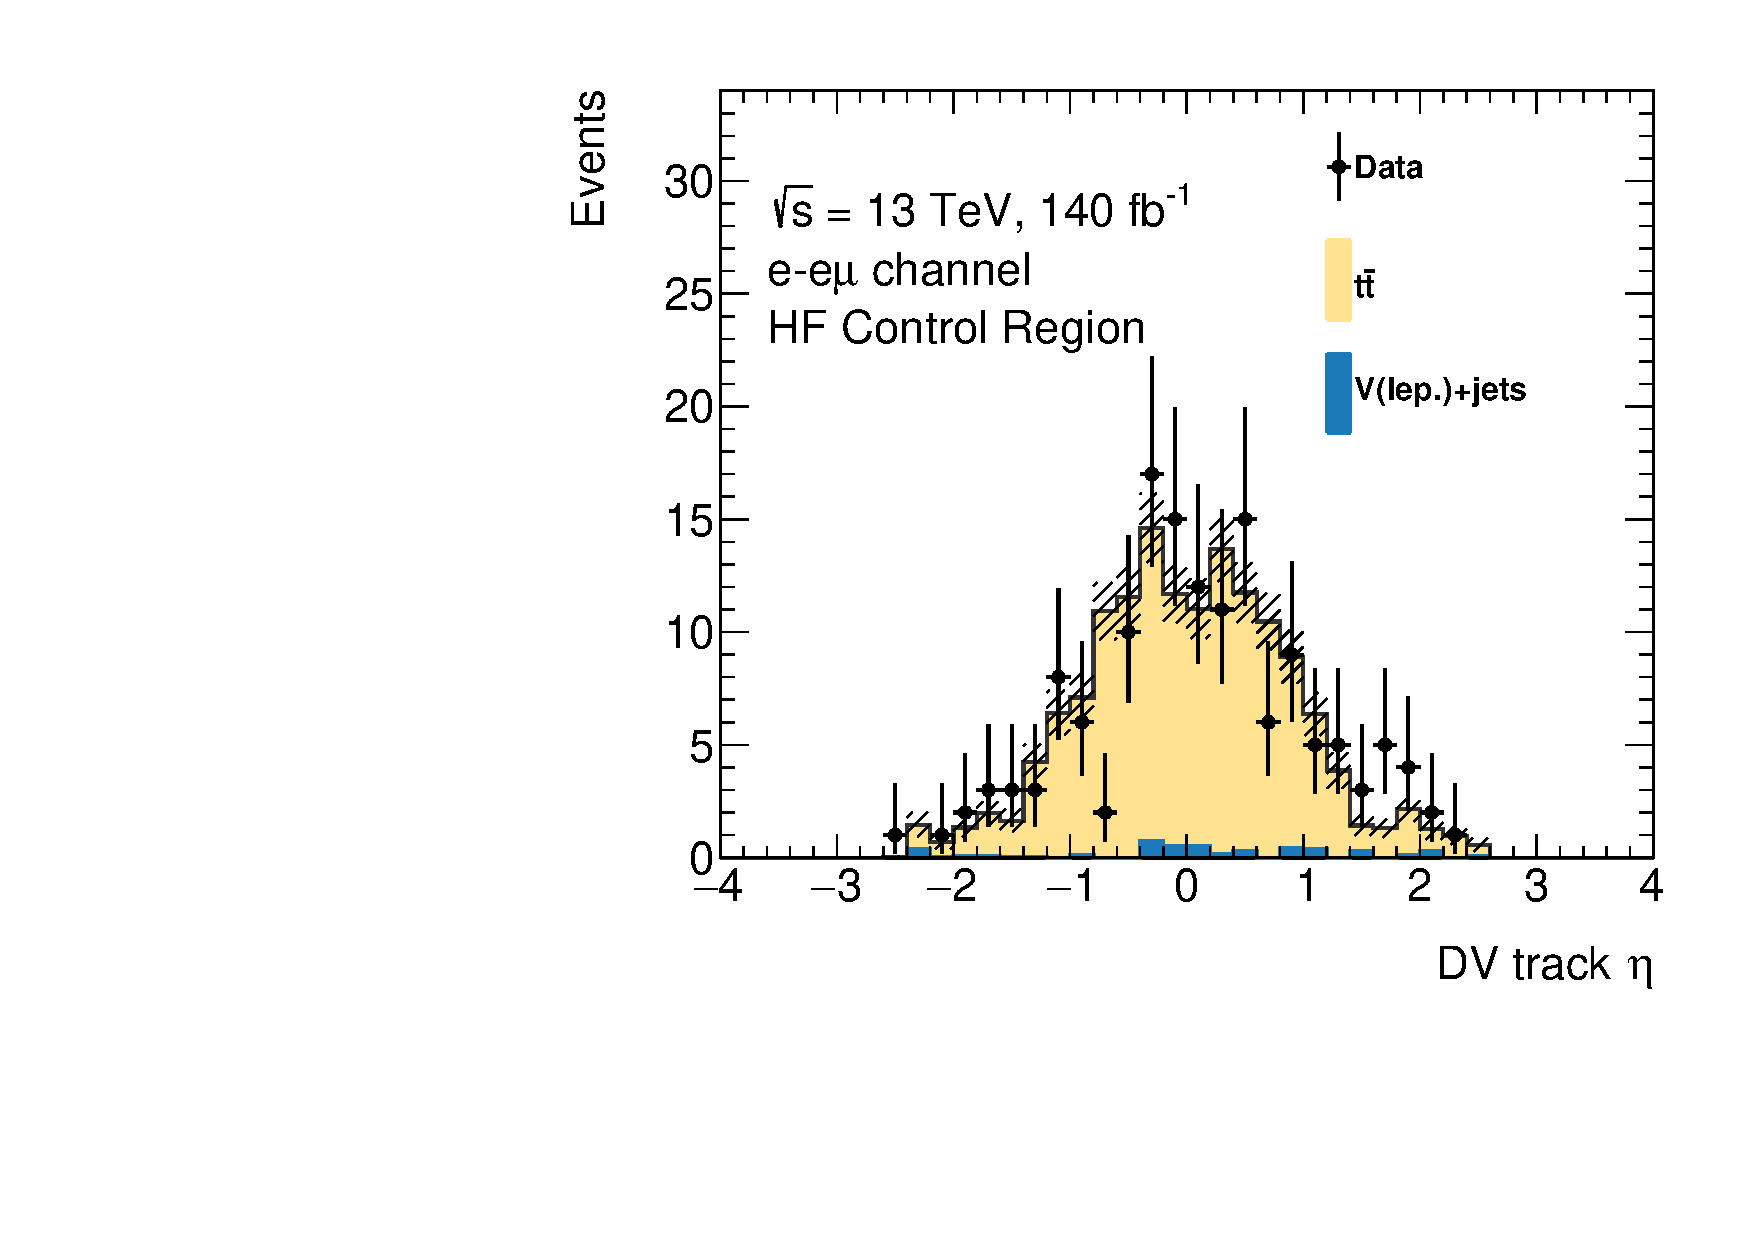
\includegraphics[width=0.24\linewidth]{figures/analysis_strategy/CR_plots/eeu/DV_trk_eta.pdf}}
    \subfloat[{$d_0$ of DV tracks [mm]}]{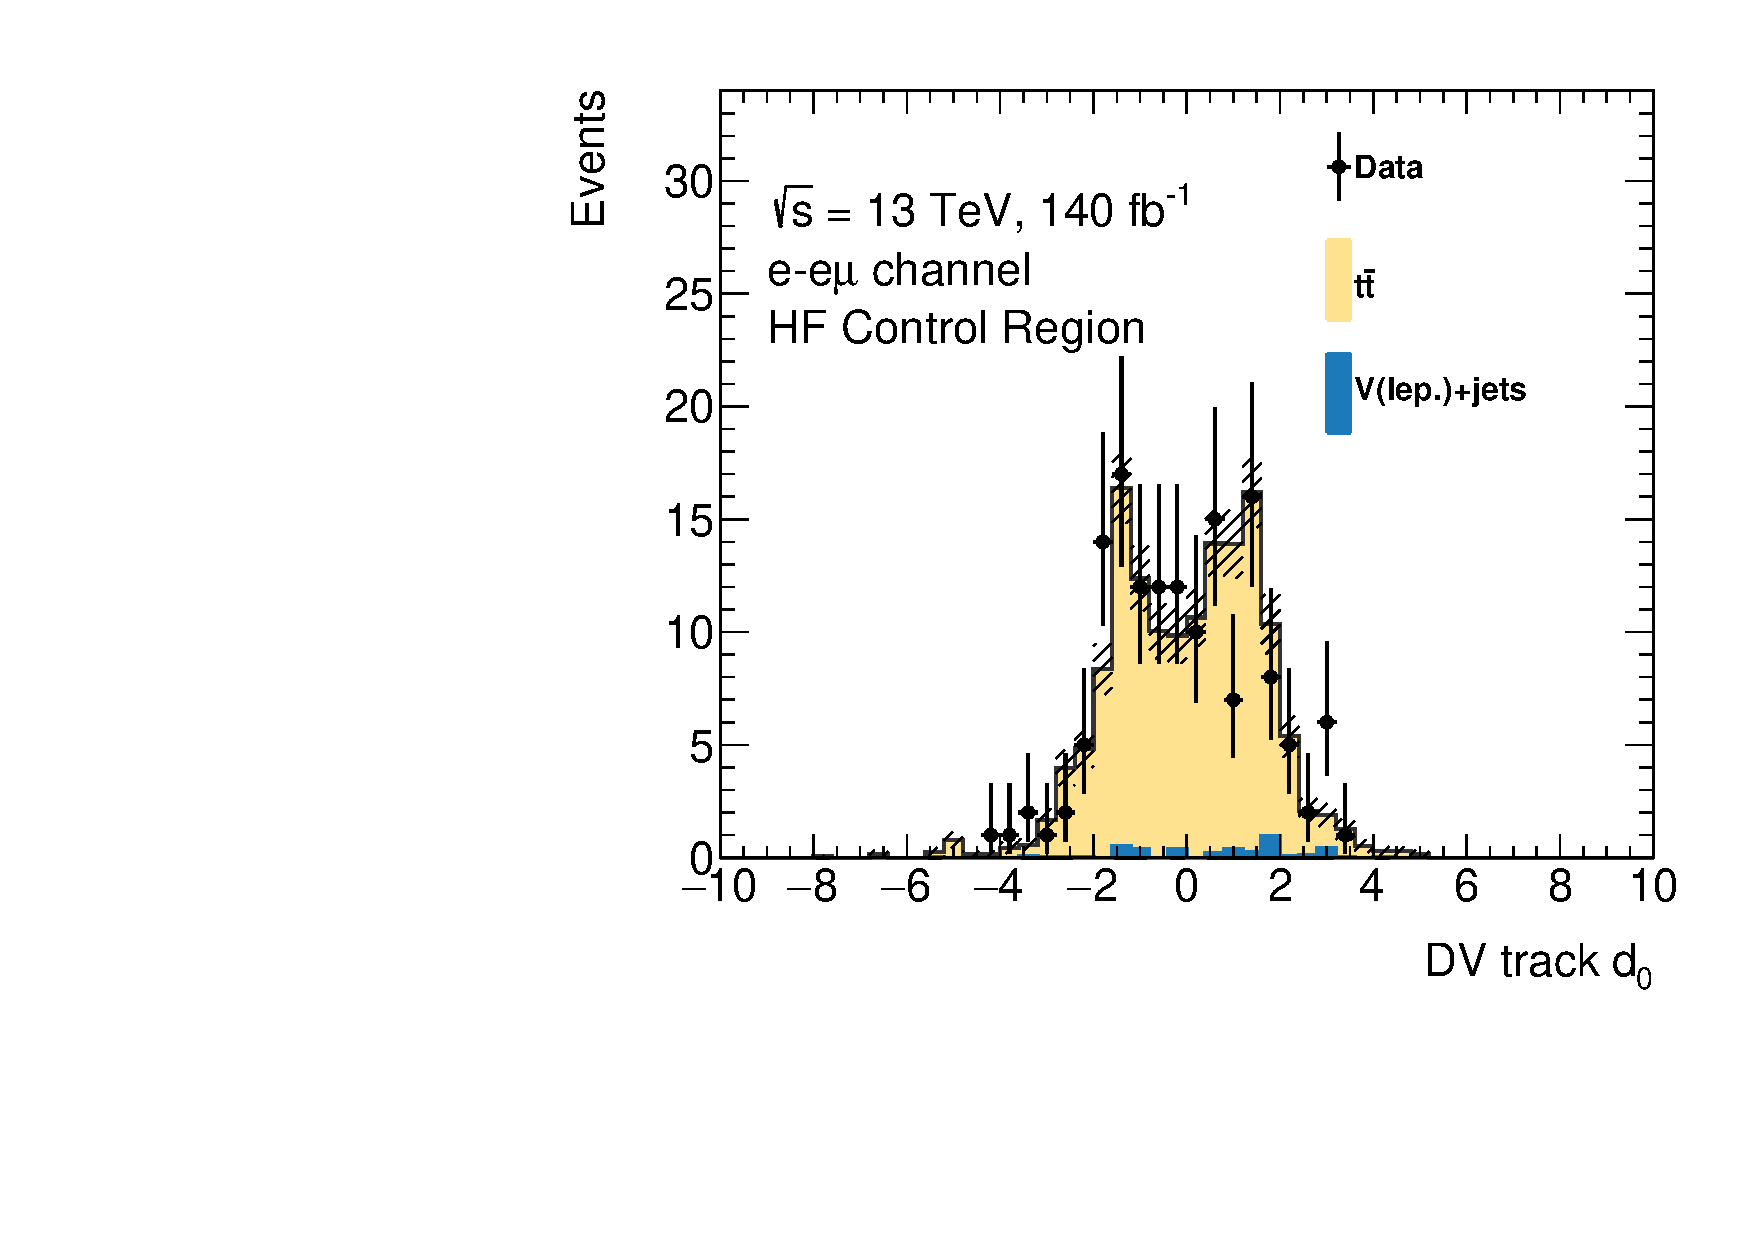
\includegraphics[width=0.24\linewidth]{figures/analysis_strategy/CR_plots/eeu/DV_trk_d0.pdf}}
    \caption{Representative kinematics of the displaced vertex, tracks in the displaced vertex, and of the prompt lepton measured in ATLAS data and modeled by MC simulations in the \eeu Heavy Flavor Control Region.}
    \label{fig:cr_plots_eeu}
\end{figure}

\begin{figure}[!ht]
    \centering
    \subfloat[{\mdv [GeV]}]{\includegraphics[width=0.24\linewidth]{figures/analysis_strategy/CR_plots/eee/DV_mass.pdf}}
    \subfloat[{$r_\mathrm{DV}$ [mm]}]{\includegraphics[width=0.24\linewidth]{figures/analysis_strategy/CR_plots/eee/DV_r.pdf}}
    \subfloat[{$\mathcal{S}$}]{\includegraphics[width=0.24\linewidth]{figures/analysis_strategy/CR_plots/eee/DV_distFromPVsigni.pdf}}
    \subfloat[{prompt lep. \pT [GeV]}]{\includegraphics[width=0.24\linewidth]{figures/analysis_strategy/CR_plots/eee/prompt_lepton_pt.pdf}}\\
    \subfloat[{$\Delta R$ DV tracks}]{\includegraphics[width=0.24\linewidth]{figures/analysis_strategy/CR_plots/eee/DV_track_dR.pdf}}
    \subfloat[{\pT of DV tracks [GeV]}]{\includegraphics[width=0.24\linewidth]{figures/analysis_strategy/CR_plots/eee/DV_trk_pt.pdf}}
    \subfloat[{$\eta$ of DV tracks}]{\includegraphics[width=0.24\linewidth]{figures/analysis_strategy/CR_plots/eee/DV_trk_eta.pdf}}
    \subfloat[{$d_0$ of DV tracks [mm]}]{\includegraphics[width=0.24\linewidth]{figures/analysis_strategy/CR_plots/eee/DV_trk_d0.pdf}}
    \caption{Representative kinematics of the displaced vertex, tracks in the displaced vertex, and of the prompt lepton measured in ATLAS data and modeled by MC simulations in the \eee Heavy Flavor Control Region.}
    \label{fig:cr_plots_eee}
\end{figure}

\FloatBarrier
\subsection{Truth classification}
As previously mentioned, the kinematics of the hadron decay background are modeled using MC simulations of $t\bar{t}$ and $V+$jets processes and the normalization is obtained from data. Other processes, such as di-boson, multi-jet, $b\bar{b}$, which could lead to the considered final state were studied, and the contribution from them was found to be negligible. Such simulations offer a way to study the physical source of the final state using the \textit{truth origin}\footnote{The truth origin of a track, an integer value ranging from 0 to 45, demarcates the nature of the particle which decayed to give the DV track using the \texttt{MCTruthClassifier}~\cite{mc-truth-web} package. The available categories can be seen in the ATLAS reconstruction framework \url{https://gitlab.cern.ch/atlas/athena/-/blob/24.0/PhysicsAnalysis/MCTruthClassifier/MCTruthClassifier/MCTruthClassifierDefs.h}.}. 
of the tracks in the DV. The truth origin is calculated by looking at the parent information of the truth-matched particle of an ID track. Based on the kind of the parent, the truth origin is delineated into a set of categories.

\begin{figure}[!ht]
    \centering
    \includegraphics[width=0.66\linewidth]{figures/analysis_strategy/mc_classifier_studies/truth_classification_example.pdf}
    \caption{Event categories based on the truth classification of tracks associated to the displaced vertex in the control region of the \uuu channel for the total MC background.}
    \label{fig:mctruth_groups}
\end{figure}

In ~\cref{fig:mctruth_groups}, an example plot shows the grouping of different kind of DVs shown for the events passing the HF-CR selection of the \uuu channel. This region has been chosen because it is a high-statistics region and it allows to clearly highlight the different contributions. The truth origin of one of the two tracks in the DV is plotted on the $x$-axis and the truth origin of the other one is plotted on the $y$-axis. As can be seen from the $z$-axis scale, the two main contributions to the total background are events with truth origins for (track 1, track 2) = (25,26) and (26, 25): these correspond to tracks associated to the decay productions of $B$- (26) and $D$-mesons (25). This is because $B$ mesons can decay into $D$ mesons plus a charged lepton. Subsequently, real leptons can also be produced in multiple steps of the $D$-meson decay-chain. Such cases are reconstructed as a single DV with two charged leptons, thus passing the selection of the analysis. The presence of additional (low quality) tracks in the decay chain are less likely to be captured by the vertexing algorithm, since the track attachment step is modified to only use tracks that pass the track seeding requirements.

Apart from the main source of HF background, some events are also found with one of the tracks having truth origin 23 or 24, corresponding to leptons originating from light hadrons or strange mesons, respectively. These can be found in the decay chains of $B$ and $D$ mesons as well. 

Another non negligible component comes from pairs of track with true origin equal to 27: these are tracks associated to the production of $c\bar{c}$ mesons, i.e. $J/\psi$ contribution. This is suppressed by the $J/\psi$ veto introduced in this round of the analysis, however it still contributes and is localised in the $m_{DV}$ distribution around 3.1 GeV.

Additional background is found to be associated to the production of heavy flavour baryons, both containing $b$- and $c$- quarks. This population of events leads to DVs in which the tracks are classified as coming from bottom meson + charm hadron or charm meson + bottom hadron. 

The last population, significantly smaller than the ones above, consist of events in which at least one the tracks associated to the displaced vertex comes from an unknown (0) origin. This reflects the presence of real $B$- or $D$-meson production which undergo subsequent decays into leptons, with the other lepton comes from either jets in the events located close to the lepton, or, less likely, directly from the underlying event or a pileup track. This category of events is negligible with respect to the others.

A very minor contribution comes from two tracks with truth origin 9, corresponding to tracks associated to the decay of $\tau$ leptons. This component is also negligible and hence ignored in the rest of the analysis.

The population of events at (0,0) is instead cases in which two uncorrelated tracks crossing and producing a secondary vertex. These events will not be taken from the MC simulated samples. Instead, a dedicated estimate of this background is performed, as is outlined in~\cref{sec:uncorr_bkg}.

Given the grouping of the events discussed above, the following two categories are defined:
\begin{enumerate}
    \item Heavy Flavour hadron production: all the events that have as truth origin of at least one track either $b$- or $c$-meson or baryon and the events that have the 27 as the truth origin of both tracks, which corresponds to $c\bar{c}$ meson production,
    \item \textit{other}: rest of the events. This category has a minor contribution and has been considered only for \textit{in itinere} data/MC plots.
\end{enumerate}

The residual contribution of the \textit{other} component, \textbf{not included in the fit templates}, is expected to be mostly covered by the random crossing background estimate, and eventually absorbed by a global MC normalisation factor which will be used to correct the prediction of the HF background component using data in the dedicated control regions.

\begin{figure}[!ht]
    \centering
    \subfloat[SR \uuu]{\includegraphics[width=0.32\textwidth]{figures/analysis_strategy/mc_classifier_studies/SR_uuu.pdf}}
    \subfloat[SR \uue]{\includegraphics[width=0.32\textwidth]{figures/analysis_strategy/mc_classifier_studies/SR_uue.pdf}}
    \subfloat[SR \uee]{\includegraphics[width=0.32\textwidth]{figures/analysis_strategy/mc_classifier_studies/SR_uee.pdf}}\\
    \subfloat[SR \euu]{\includegraphics[width=0.32\textwidth]{figures/analysis_strategy/mc_classifier_studies/SR_euu.pdf}}
    \subfloat[SR \eeu]{\includegraphics[width=0.32\textwidth]{figures/analysis_strategy/mc_classifier_studies/SR_eeu.pdf}}
    \subfloat[SR \eee]{\includegraphics[width=0.32\textwidth]{figures/analysis_strategy/mc_classifier_studies/SR_eee.pdf}}
    \caption{Truth origin distributions of track pairs associated to displaced vertices in the six leptonic signal region channels for the total MC background.}
    \label{fig:truth_origin_SR}
\end{figure}

~\Cref{fig:truth_origin_SR} shows the truth origin distribution for the total MC prediction for the SRs in the six channels. The background composition is very similar to that in the \uuu HF-CR, with the production of heavy-flavour hadrons being the leading contribution. One notable difference between the \uuu HF-CR, discussed previously, and the SR, discussed here, is that there are almost no events with tracks with unknown truth origin (0). This is related to the fact that in the signal regions the two reconstructed leptons matched to the tracks associated to the DV are required to be isolated. Such a requirement reduces the probability that one real lepton produced in a DV is associated to a random track coming from a jet close-by.

\begin{figure}[!ht]
    \centering
    \subfloat[HF-CR \uuu]{\includegraphics[width=0.32\textwidth]{figures/analysis_strategy/mc_classifier_studies/CR_SM_uuu.pdf}}
    \subfloat[HF-CR \uue]{\includegraphics[width=0.32\textwidth]{figures/analysis_strategy/mc_classifier_studies/CR_SM_uue.pdf}}
    \subfloat[HF-CR \uee]{\includegraphics[width=0.32\textwidth]{figures/analysis_strategy/mc_classifier_studies/CR_SM_uee.pdf}}\\
    \subfloat[HF-CR \euu]{\includegraphics[width=0.32\textwidth]{figures/analysis_strategy/mc_classifier_studies/CR_SM_euu.pdf}}
    \subfloat[HF-CR \eeu]{\includegraphics[width=0.32\textwidth]{figures/analysis_strategy/mc_classifier_studies/CR_SM_eeu.pdf}}
    \subfloat[HF-CR \eee]{\includegraphics[width=0.32\textwidth]{figures/analysis_strategy/mc_classifier_studies/CR_SM_eee.pdf}}
    \caption{Truth origin distributions of track pairs associated to displaced vertices in the six leptonic control region channels for the total MC background.}
    \label{fig:truth_origin_CR}
\end{figure}

\begin{comment}
~\Cref{fig:truth_origin_CR} shows the truth origin distribution for the total MC prediction for the SRs in the six channels. The background compositions are similar in the HF-CRs across all six channels as well as to the SRs, with the production of heavy-flavour hadrons being the leading contribution. The presence of a minor component of events categorised as production of heavy-flavour baryons is related to the fact that, in the HF-CRs, at least one of the two displaced leptons is required to be non-isolated.

{\color{red}
\begin{figure}[!ht]
    \centering
    \subfloat[SR \uuu]{\includegraphics[width=0.32\textwidth]{figures/analysis_strategy/mc_classifier_studies/dataMCplots/SR/inclusive_count_of_events_uuu.pdf}}
    \subfloat[SR \uue]{\includegraphics[width=0.32\textwidth]{figures/analysis_strategy/mc_classifier_studies/dataMCplots/SR/inclusive_count_of_events_uue.pdf}}
    \subfloat[SR \uee]{\includegraphics[width=0.32\textwidth]{figures/analysis_strategy/mc_classifier_studies/dataMCplots/SR/inclusive_count_of_events_uee.pdf}}\\
    \subfloat[SR \euu]{\includegraphics[width=0.32\textwidth]{figures/analysis_strategy/mc_classifier_studies/dataMCplots/SR/inclusive_count_of_events_euu.pdf}}
    \subfloat[SR \eeu]{\includegraphics[width=0.32\textwidth]{figures/analysis_strategy/mc_classifier_studies/dataMCplots/SR/inclusive_count_of_events_eeu.pdf}}
    \subfloat[SR \eee]{\includegraphics[width=0.32\textwidth]{figures/analysis_strategy/mc_classifier_studies/dataMCplots/SR/inclusive_count_of_events_eee.pdf}}
    \caption{Inclusive count of events for each of the six leptonic signal regions, divided by the truth classification method. The hatched band represents the MC statistical uncertainty only.}
    \label{fig:truth_origin_SR_inc}
\end{figure}

~\Cref{fig:truth_origin_SR_inc} shows the expected number of events for the signal regions in each of the six channels, diving the MC events based on the truth categories defined previously in this section. As can be seen, the $c\bar{c}$ production component is only present in the channels with SFOS leptons in the DVs. The larger contribution of the \textit{other} component observed in the $x-ee$ channels with respect to $x-x\mu$ channels is due to the difference in identification working points chosen for electrons and muons, with the one for electrons being much looser, thus more subject to be faked by a random track crossing associated to the DV.
These regions (signal regions) are currently blinded.
}

\begin{figure}[!ht]
    \centering
    \subfloat[HF-CR \uuu]{\includegraphics[width=0.32\textwidth]{figures/analysis_strategy/mc_classifier_studies/dataMCplots/CR/inclusive_count_of_events_uuu.pdf}}
    \subfloat[HF-CR \uue]{\includegraphics[width=0.32\textwidth]{figures/analysis_strategy/mc_classifier_studies/dataMCplots/CR/inclusive_count_of_events_uue.pdf}}
    \subfloat[HF-CR \uee]{\includegraphics[width=0.32\textwidth]{figures/analysis_strategy/mc_classifier_studies/dataMCplots/CR/inclusive_count_of_events_uee.pdf}}\\
    \subfloat[HF-CR \euu]{\includegraphics[width=0.32\textwidth]{figures/analysis_strategy/mc_classifier_studies/dataMCplots/CR/inclusive_count_of_events_euu.pdf}}
    \subfloat[HF-CR \eeu]{\includegraphics[width=0.32\textwidth]{figures/analysis_strategy/mc_classifier_studies/dataMCplots/CR/inclusive_count_of_events_eeu.pdf}}
    \subfloat[HF-CR \eee]{\includegraphics[width=0.32\textwidth]{figures/analysis_strategy/mc_classifier_studies/dataMCplots/CR/inclusive_count_of_events_eee.pdf}}
    \caption{Inclusive count of events for each of the six Heavy Flavor Control Regions, divided by the truth classification method. The hatched band represents the MC statistical uncertainty only. The black dots represent ATLAS Run-2 data.}
    \label{fig:truth_origin_CR_inc}
\end{figure}

~\Cref{fig:truth_origin_CR_inc} shows the expected number of events for the HF-CRs in each of the six channels, diving the MC events based on the truth categories defined previously in this section. Also in this case, as for the SR, the $c\bar{c}$ production component is only prevalent in the channels with SFOS displaced leptons. The same comment about the \textit{other} component holds as well. Overall, the total number of events predicted by the MC simulation matches, within uncertainty, to what is observed in data.
\end{comment}

\subsection{Background prediction}
To exploit the fact that the different background components have different DV mass distributions, the chosen variable  in the HF-CRs for the statistical analysis, described later in~\cref{sec:sig_ext}, is \mdv itself. On the other hand, since the HNL signal extraction is done from the SRs, the reconstructed HNL mass (\mhnl) introduced in the 2022 analysis (details of calculation in~\cref{chap:HNL_mass} of the appendix) is used for its strong discrimination power. The reconstruction uses energy-momentum conservation in the HNL production ($W\to\mathcal{N}\ell_1$) and decay ($\mathcal{N}\to\ell_1\ell_2\nu$) to get around the lack of measurement of the neutrino kinematics. The MC samples are used to build the templates of predictions used in the statistical analysis.~\Cref{fig:mhnl_signal} shows the reconstructed \mhnl for signal samples with various simulated masses and $\ctau = 10$~mm. The \mhnl resolution for channels with $\mu\mu$ DVs is the best, followed by $\mu e$ and $ee$ DVs. This is due to the use of the kinematics of the track object and not of the lepton object in the reconstruction of this variable. Since GSF tracks don't fully account for radiation losses from electrons, they give a worse momentum measurement of the HNL decay products, and hence a worse reconstructed \mhnl value.

\begin{figure}[!ht]
    \centering
    \subfloat[\uuu]{\includegraphics[width=0.32\textwidth]{figures/analysis_strategy/uuu_mHNL.pdf}}
    \subfloat[\uue]{\includegraphics[width=0.32\textwidth]{figures/analysis_strategy/uue_mHNL.pdf}}
    \subfloat[\uee]{\includegraphics[width=0.32\textwidth]{figures/analysis_strategy/uee_mHNL.pdf}}
    \caption{Reconstructed \mhnl distributions for signal samples with $\ctau = 10$~mm. The signals are scaled to arbitrary values for side-by-sde comparison between different mass points.}
    \label{fig:mhnl_signal}
\end{figure}

The available statistics from MC simulations is sufficient in the HF-CRs, therefore, the expected background MC events are used. A systematic uncertainty equal to the relative statistical uncertainty of the background MC predictions is assigned to this template. In the HF predictions in the SR, instead, some un-physical statistical fluctuations are observed. Furthermore, insufficient statistics in the SR from the MC samples lead to no background prediction beyond $\mhnl=7$~GeV. In order to reduce the impact of such artefacts, the shape of the \mhnl distribution of the HF background in the SR is obtained from a shape region (ShR) with requirements on the DV lepton isolation and $m_{\ell\ell\ell}$ removed. Since similar kinematics and compositions are observed in all the regions for this background, events from the ShR of all six channels are combined to obtain the shape. Finally, the shape is scaled back to the event yield predicted by MC simulations in the six individual channels. A dedicated systematic uncertainty is assigned to this method to cover the assumptions made with the details mentioned in~\cref{sec:sig_ext}.
 
\begin{figure}[!ht]
    \centering
    \includegraphics[width=\linewidth]{figures/analysis_strategy/template_building/template_building_SR.pdf}
    \caption{Template building method used for the HF background in the Signal Regions.}
    \label{fig:template_building}
\end{figure}

~\Cref{fig:template_building} shows the template building procedure for the HF background component in the SR. It shows the merging of the six different channels (bottom row), first in \xuu, \xue and \xee channels (middle row), and then all the channels merged (top plot). The yield from ShR in each case is shown, normalized to the nominal MC event yield for a one-to-one shape comparison. The original MC at each level is shown with black dots and the shape from ShR normalized to the original MC in individual channels in shown in dashed red lines. For the sake of illustration, the ShR shape at the DV flavor level is also shown in blue, however this shape is not used directly in the analysis. Finally, the shape from the ShR for all channels combined, which is used as the SR background estimate shape in the SR, is shown by the green line. The agreement between the original MC predictions and the ShR shape is sufficiently good across all channels in the $\mhnl=1-7$~GeV range, with the ShR prediction also giving a non-zero prediction in the tails of the distribution, i.e. in the $\mhnl=7-20$~GeV range. The templates obtained with this method are shown in~\cref{fig:templates_hf_sr}. 

\begin{figure}[!ht]
    \centering
    \subfloat[SR \uuu]{\includegraphics[width=0.32\textwidth]{figures/analysis_strategy/template_building/HF_SR_uuu_fitTemplate_MergeDVtype_multiComp.pdf}}
    \subfloat[SR \uue]{\includegraphics[width=0.32\textwidth]{figures/analysis_strategy/template_building/HF_SR_uue_fitTemplate_MergeDVtype_multiComp.pdf}}
    \subfloat[SR \uee]{\includegraphics[width=0.32\textwidth]{figures/analysis_strategy/template_building/HF_SR_uee_fitTemplate_MergeDVtype_multiComp.pdf}}\\
    \subfloat[SR \euu]{\includegraphics[width=0.32\textwidth]{figures/analysis_strategy/template_building/HF_SR_euu_fitTemplate_MergeDVtype_multiComp.pdf}}
    \subfloat[SR \eeu]{\includegraphics[width=0.32\textwidth]{figures/analysis_strategy/template_building/HF_SR_eeu_fitTemplate_MergeDVtype_multiComp.pdf}}
    \subfloat[SR \eee]{\includegraphics[width=0.32\textwidth]{figures/analysis_strategy/template_building/HF_SR_eee_fitTemplate_MergeDVtype_multiComp.pdf}}
    \caption{Comparison of the original MC predictions and different smoothed predictions for the HF background in the Signal Regions.}
    \label{fig:templates_hf_sr}
\end{figure}


\section{Uncorrelated Background}\label{sec:uncorr_bkg}
The Random Crossing background consists of a pair of uncorrelated tracks crossing each other in space and accidentally getting reconstructed as a DV paired with a prompt lepton to yield an event in our measured phase space. These exact characteristics of the RC background are used to estimate them, the method for which was developed for~\cite{Barlow:1749971}.~\Cref{fig:rc_method} illustrates the steps used to create RC DV candidates in a data driven manner.

\begin{figure}[!ht]
    \centering
    \includegraphics[width=\textwidth]{figures/analysis_strategy/random_crossing/rtc_scheme.png}
    \caption{Schematic illustration of track pool creation from different events used to create randomly paired tracks for artificial vertex creation to estimate the random track crossing background.}
    \label{fig:rc_method}
\end{figure}

In the first step, a pool of tracks passing the track selection requirements of VSI is created from all available data events. From this pool, track pairs are randomly selected (with replacement) which are required to come from different events. In the last step, these track pairs are passed through VSI and a DV reconstruction is attempted. The result is a set of artificial DVs representative of the vertices expected to result from random track crossings.

The probability to obtain a DV from a track pair ($p(\text{DV|pair})$) is given by:
\begin{equation}
    p(\text{DV|pair}) \approx \lim_{N_\text{Attempts}\to \infty}\frac{N_\text{DV}}{N_\text{Attempts}}.
\end{equation}
where $N_\text{Attempts}$ is the number of times a DV reconstruction is attempted using track pairs and $N_\text{DV}$ is the number of times a DV was successfully reconstructed in the attempts. The number of predicted RC DVs ($N_\text{Predicted crossings}$), hence, follows as:
\begin{equation}\label{eq:crossings}
    N_\text{Predicted crossings} = p(\text{DV}|\text{Pair}) \times N_\text{Real} = N_{DV} \times \frac{N_\text{Real}}{N_\text{Attempts}}.
\end{equation}
Therefore, each artificially reconstructed RC DV is weighted by a factor $\frac{N_\text{Real}}{N_\text{Attempts}}$, where $N_\text{Real}$ is the number of combinatorial track pairs found in data. Care is taken to ensure that~\cref{eq:crossings} are representative of unrelated track pairs. Correlated track pairs from decaying resonances should not enter $N_\mathrm{Real}$, as such pairs do not occur randomly, and the DV that may result from them are estimated using dedicated other techniques. To ensure this, both $N_\mathrm{Real}$ and $N_\mathrm{Attempts}$ are obtained by counting pairs with $m_\mathrm{Pair}>6$~GeV to reject low-mass hadron decays, and $|\Delta\phi_\mathrm{Pair}|>2.4$ to reject Drell-Yan and resonant $Z$ decay events. In addition, the normalisation is performed separately for events that contain prompt leptons and events that don’t. The normalisation weights are obtained separately for each DV flavor.

Finally, the RC DV candidate is combined with the prompt lepton (which is required to come with one of the tracks in the pool) to yield a complete signature defining the RC background in this search. The kinematics of this 3-lepton system are then used to reconstruct variables that this analysis is sensitive to, such as \mdv and \mhnl.

The kinematics and normalization of the RC estimate are successfully validated in a phase space rich in this background. The $m_{\ell\ell\ell}$ pre-selection is removed, the fiducial volume cut is relaxed ($2\text{ mm}<\rdv<300\text{ mm}$, and an added high \mdv ($>2$~GeV) requirement is imposed. From this phase space, all events passing the SR cuts are veto-ed to define the validation region. The background is found to be extremely suppressed with very low expected yields in all regions, as shown in~\cref{tab:rc_yields}. 

\begin{table}[!htbp]
    \centering
    \begin{tabular}{c|c|c|c|c|c|c|c}
    \hline\hline
        Region & \uuu & \uue & \uee & \euu & \eeu & \eee & Total\\
        \hline
        SR & .025 & .017 & .000 & .002 & .030 & .048 & .123  \\
        HF-CR & .560 & .227 & .044 & .123 & .154 & .380 & 1.489 \\
        \hline \hline
    \end{tabular}
    \caption{Total yields of random crossing backgrounds in the signal and HF control regions for the six channels.}
    \label{tab:rc_yields}
\end{table}


\section{Signal Extraction}\label{sec:sig_ext}
As previously mentioned, six channels are used in this analysis, and a global signal strength is extracted from all channels for each model. Depending on the model being considered, an HNL signal may or may not have contributions in a certain channel. For instance, a $\mu$ only mixing HNL will have events in the \uuu SR, but not in the \euu SR, since the prompt lepton and the displaced leptons have different flavors in the latter. This fact is used to use the SRs in certain channels to help constrain the HF background along with the CRs. Due to the extremely low HF background contribution in the \eee and \uee SRs, they are combined in the fit to an \xee SR.~\Cref{tab:fit_structure} shows the primary use of the SRs and HF-CRs defined in the analysis for each channel considered. This section outlines the uncertainties considered in the analysis and the structure of the statistical analysis used to extract the global signal strength.

%\begin{landscape}
    \begin{table}[!htbp]
        \footnotesize
        \centering
        %\setlength\extrarowheight{6pt}
        \resizebox{\columnwidth}{!}{
        \begin{tabular}{c|c|c|c|c|c|c}
        \hline\hline
           \multirow{2}{*}{Model} & \multicolumn{5}{c|}{Signal Region}  &  Heavy Flavor Control Region\\
           \cline{2-7}
           & \uuu & \uue & \euu & \eeu & \xee & All Channels \\
           \hline
           1SFH($\mu$) & {\color{green} Signal} & {\color{green} Signal} & {\color{red} Background} & {\color{red} Background} &  {\color{green} Signal} &  \multirow{4}{*}{{\color{red} Background}} \\
           %\cline{1-6}
           1SFH($e$) & {\color{red} Background} & {\color{red} Background} &  {\color{green} Signal} &  {\color{green} Signal} & {\color{green} Signal} &  \\
           %\cline{1-6}
           2QDH(IH) & {\color{green} Signal} & {\color{green} Signal} & {\color{green} Signal} & {\color{green} Signal} & {\color{green} Signal} &  \\
           %\cline{1-6}
           2QDH(NH) & {\color{green} Signal} & {\color{green} Signal} & {\color{green} Signal} & {\color{green} Signal} & {\color{green}       Signal} & \\
           \hline \hline
         \end{tabular}
         }
     \caption{A summary of the use of the fit regions defined for the models that are used in the interpretation of the analysis results. {\color{green} Signal} represents when a region is mainly used for signal extraction, and {\color{red} Background} represents when a region is used for constraining the background from Heavy Flavor decays.}
     \label{tab:fit_structure}
\end{table}
%\end{landscape}

\subsection{Uncertainties}
All relevant sources of uncertainties are considered in this analysis which can affect the estimate on the background and signal MC predictions. One standard deviation ($\pm 1 \sigma$) variations are considered for all uncertainties, and are propagated to the statistical fit. The standardization of LRT objects in this version of the analysis allowed for a better understanding of the uncertainties on these objects in close coordination with the Combined Performance (CP) groups. The use of MC simulations for the modeling of HF decay background warranted an inclusion of the theoretical modeling uncertainties on them, which have been estimated using the prescription from the Physics Modeling Group. This section describes all the sources of systematic uncertainties considered in this analysis. The net impact of the systematic uncertainties on the analysis is shown in~\cref{tab:uncertainty}. Systematics are found the be a sub-dominant source of uncertainties and the results are limited by the statistical size of the dataset.

\subsection*{Integrated Luminosity}
The LUCID2 detector was used to measure the integrated luminosity collected by ATLAS during Run-2 with a central value of 140.1 pb$^{-1}$ and an error of 0.83\%~\cite{DAPR-2021-01}.

\subsection*{Pileup}
While pileup is modeled in simulation, the simulated collision conditions are not identical to those experienced during the data collection. A centrally managed tool is used to re-weight signal and background MC events and take into account the impact of pileup during the various data periods.

\subsection*{Trigger}
The efficiency of triggering by a muon or an electron in MC is adjusted to that in data by looking at $Z\to\ell\ell$ events. The efficiency calibrations from the CP groups are used to account for these uncertainties on the primary triggering object, which is the prompt lepton in this analysis.

\subsection*{Lepton Momentum}
The momentum of the leptons measured in MC are calibrated for detector conditions using Z and $J/\psi$ decays. The standard CP efficiency calibrations are used for all leptons used in this analysis.

\subsection*{Lepton Reconstruction and Identification}
The muons in this analysis are either standard or LRT, all accepted using the \texttt{Medium} identification WP. For standard muons, the standard CP efficiency calibrations are applied obtained using $Z(J/\psi)$ decays for muon $\pT >(<)\,10$~GeV in a tag and probe analysis~\cite{MUON-2018-03}. 
For LRT muons, the reconstruction and identification efficiencies are studied separately and are measured indirectly. The efficiency to measure a \texttt{Medium} muon can be divided into two factors:
\begin{equation}
    \epsilon\, (\text{Medium }\mu) \approx \epsilon\, (\text{Medium }\mu \,|\,\mathrm{ID}) \times \epsilon (\mathrm{ID}),
\end{equation}
Here, $\epsilon\, (\text{LRT ID})$ is roughly estimated using $K_S\to\pi^+\pi^-$ decays~\cite{IDTR-2021-03}. Furthermore, it is postulated that
\begin{equation}
    \epsilon\, (\text{Medium LRT }\mu \,|\,\text{LRT ID})\approx\epsilon\, (\text{Medium Standard }\mu \,|\,\text{Standard ID}),
\end{equation}
since the MS is \textit{far} from the IP, and hence is insensitive to cm level displacements that come from the difference in Standard and LRT ID track reconstruction. The above two inferences allow for the calibration of LRT muon reconstruction and identification efficiencies using the same $Z$ and $J/\psi$ decays, since $\epsilon\, (\text{Medium Standard }\mu \,|\,\text{Standard ID})$ is measured by the standard tag and probe method with the ID track corrections (i.e. contribution from $\epsilon\, (\text{Standard ID})$) disabled in the measurement.

After studying the above terms, an uncertainty of $1(3)\%$ is applied on LRT muons with $\pT >(<)\,5$~GeV.

A similar decomposition also applies to the reconstruction and identification of electrons, where separate reconstruction efficiencies are calculated for standard and LRT electrons. For the identification criteria, separate efficiencies are applied to the prompt electron and the displaced electron, since they use the \texttt{Medium} and \texttt{VeryLooseNoPix} identification WPs, respectively.

The electron reconstruction efficiency is accounted with a 3\% uncertainty for both the standard and LRT objects. The \texttt{Medium} electron identification efficiency is measured with a 4\% uncertainty, and \texttt{VeryLooseNoPix} electrons are identified with a 5\% uncertainty.

\subsection*{Lepton Isolation}
The CP efficiency calibrations are used on the calibration of the isolation applied on the prompt and displaced muons, while a conservative 2\% uncertainty is applied on the electron isolation efficiency. Since the same working point is applied on standard and LRT objects without modifications, the same uncertainties are applied to both of them.

\subsection*{Flavor Tagging}
Uncertainties from the measurement of the jet energy scale and resolution were found to have no impact on this analysis. The systematic uncertainties from the calibration of the flavor tagging algorithm are considered using the medium reduction scheme, as recommended by the flavor tagging CP group.

\subsection*{Signal Modeling}
In the 2022 analysis, the HNL process was modeled at LO using \textsc{Pythia}, and the MC prediction was attached a modeling uncertainty of $3\% \oplus 5\%$, with the former coming from the measurement of the $W$ production cross section and the latter from the analytical calculation of the HNL branching fraction compared to the prediction from \textsc{MadGraph5}. It was found that the spin correlations of the HNL decay products were not well modeled by \textsc{Pythia}, and a dedicated reweighting procedure was applied to adjust for the same. In this analysis, the predictions are modeled at NLO with the spin correlation well modeled by the MC event generators. Hence, a reduced yet conservative uncertainty of 5\% is considered on the signal prediction.

\subsection*{Random Crossing Modeling}
The random crossing background estimate reuses ID tracks to create a preliminary track pool, which are later used to reconstruct DVs with uncorrelated objects. The statistical correlation coming from such a multi-count is accounted using a bootstrapping~\cite{ATL-PHYS-PUB-2021-011} mechanism. Furthermore, alternate track sampling methods account for uncertainties coming from the bias in the sampling strategy of such tracks. A conservative 50\% uncertainty is applied on the random crossing background estimate to cover the above effects. Given the very small contribution of this background in all the considered regions, this uncertainty is expected to have a negligible effect.

\subsection*{HF Background Modeling}
As described in~\cref{sec:data_mc_samples}, $t\bar{t}$ and $V+$jets MC samples are used to model the background from HF decays. Theoretical uncertainties are evaluated for both of these MC simulations following the recommendations of the ATLAS Physics Modeling Group:
\begin{itemize}
    \item $\mathbf{t\bar{t}}$: Uncertainties are evaluated for the hard scatter generation (or matrix element calculation), parton showering process, QCD scale, modeling of the initial and final state radiations, and the choice of the parton density function.

    The matrix element uncertainty is evaluated using a two-point comparison between the nominal \textsc{Powheg} sample showered with \textsc{Pythia\,8} and a sample generated with an identical configuration except the \texttt{pThard} parameter of \textsc{Powheg} set to 1 instead of the nominal value of 0. The parton shower uncertainty is evaluated using a two-point comparison between the nominal \textsc{Powheg} sample showered with \textsc{Pythia\,8} and \textsc{Herwig,7} showering program.

    QCD scale uncertainty is evaluated using the five-point envelope of the variations of renormalization and factorization scales by factors of 2.0 or 0.5 (removing the cases when both are 0.5, both are 2, and one is 2.0 and the other is 0.5). The initial and final state radiation uncertainties are calculated using the $\pm 1 \sigma$ weights from \textsc{Pythia\,8}. Lastly, the PDF uncertainty is evaluated using the \textsc{NNPDF3.0nlo} variations in the \textsc{Powheg+Pythia\,8} sample as defined in the \texttt{PDF4LHC} recommendations~\cite{Butterworth_2016}.

    \item $\mathbf{V+}$\textbf{jets}: Uncertainties are evaluated for the QCD scale and parton density function choice.

    QCD scale uncertainty is evaluated using the seven-point envelope of the variations of renormalization and factorization scales by factors of 2.0 or 0.5 (removing the cases when both are 0.5 and both are 2). The PDF uncertainty is evaluated in the same manner as for the $t\bar{t}$ samples following the \texttt{PDF4LHC} recommendations.
\end{itemize}
~\Cref{tab:sys_theo} summarizes the theory uncertainties used for the background modeling and the method used to calculate them.

  \begin{table}[!htbp]
  {
    \begin{tabular}{clcc}
      \hline\hline
      Process & Uncertainty & Variations & Method\\
      \hline
      $t\bar{t}$    & Matrix Element & \textsc{Powheg}+\textsc{Pythia\,8} \texttt{pThard}:0,  & Two-point variation\\
      & & \textsc{Powheg}+\textsc{Pythia\,8} \texttt{pThard}:1 & \\
      & Parton Shower & \textsc{Powheg}+\textsc{Pythia\,8},  & Two-point variation\\
      & & \textsc{Powheg}+\textsc{Herwig\,7} & \\
      & Initial State Radiation & Var3cUp, Var3cDown & up down variation \\
      & Final State Radiation & muRfac=2.0, muRfac=0.5 & up down variation \\
      & QCD Scale &  $\mu_R,\,\mu_F\in\{.5,\,1,\,2\}$ & 5-point envelope \\
      & PDF & NNPDF30\_nlo\_as\_0118 & $\sqrt{\frac{1}{N} \sum_i\left(X_i-X_0\right)^2}$\\
      \hline
      $V$+jets & QCD Scale & $\mu_R,\,\mu_F\in\{.5,\,1,\,2\}$ & 7-point envelope \\
      & PDF & NNPDF30\_nlo\_as\_0118 & $\sqrt{\frac{1}{N} \sum_i\left(X_i-X_0\right)^2}$\\
      \hline
      \hline
    \end{tabular}
    }
    \centering
    \caption{Summary of the theoretical systematic uncertainties considered on the background Monte Carlo simulations and their method of evaluation.}
    \label{tab:sys_theo}
  \end{table}

\subsection*{HF Template Building}
As described previously, a dedicated uncertainty is assigned on the template building process of the HF background. It is equal to the Monte Carlo Statistics uncertainty in the HF-CR, since no smoothing or shape building process is applied in those regions. In the SR, a two-point uncertainty comparing the ShR shape from a single channel and the ShR shape from the combination of all channels is applied. Since the shapes are normalized to the MC event yield of individual channels, this is a shape-only effect.

\subsection*{Monte Carlo Statistics}
Lastly, the MC statistics uncertainty is considered on the signal prediction as well coming from the limited statistics considered in the production of the signal MC samples.

\subsection{Simultaneous fit}
A global likelihood minimizing fit is performed to extract a signal strength for each simulated signal point. A likelihood function $\mathcal{L}$ is used to define a global probability density function of this measurement. The extended likelihood $\mathcal{L}$ consists of a product of likelihood functions ($\mathcal{P}$s) of the SR yield and CR yield. The function is shown without a channel indexing for simplicity, but a global product runs over all five SRs and six CRs considered in the analysis:
\begin{equation}
\label{eqn:likelihood}
    \mathcal{L} = \mathcal{P}( N_{\mathrm{data}}^{\mathrm{SR}}| \mu \cdot N_{\mathrm{signal}}^{\mathrm{SR}} + 
    \mu_{\mathrm{HF}}  \cdot N_{\mathrm{HF}}^{\mathrm{SR}} + N_{\mathrm{RC}}^{\mathrm{SR}} ) \cdot 
    \mathcal{P}(N_{\mathrm{data}}^{\mathrm{CR}} | \mu_{\mathrm{HF}}\cdot N_{\mathrm{HF}}^{\mathrm{CR}} + N_{\mathrm{RC}}^{\mathrm{CR}}) \cdot                                                    \prod_{i=1}^{n_{\theta_i}}\mathrm{N}(\tilde{\theta_i}| \theta_i),
\end{equation}

where $N_{\mathrm{data}}^{\mathrm{SR}}$ and $N_{\mathrm{data}}^{\mathrm{CR}}$ are the numbers of events observed in data in the signal region and the HF control region, respectively, and $N_{\mathrm{signal}}^{\mathrm{SR}}$ is the expected signal yield in the SR. The parameter $\mu$ is the normalization of the signal, and $\mu_{\mathrm{HF}}$ that of the HF background. A signal strength of $\mu=0$ corresponds to a background only hypothesis while $\mu=1$ corresponds the nominal signal plus background (S+B) hypothesis. $N_{\mathrm{HF}}^{\mathrm{SR}}$ and $N_{\mathrm{HF}}^{\mathrm{CR}}$ are the expected numbers of HF background events in the SR and CR, respectively. As previously mentioned, the RC background is taken directly from the data-driven prediction and is represented by $N_{\mathrm{RC}}^{\mathrm{SR}}$ and $N_{\mathrm{RC}}^{\mathrm{CR}}$ in the SR and CR, respectively.  The term $\mathcal{N}$ is a normal distribution that parameterizes the systematic effect of the type $i$ as a function of a Gaussian constrained nuisance parameter $\theta_i$ and the associated estimate of the corresponding effect $\tilde{\theta_i}$, as mentioned in the previous section. 

The parameter $n_{\theta_i}$ represents the number of nuisance parameters modeling the systematic uncertainties considered in this analysis. The likelihood function $\mathcal{P}$ in the SR and CR are defined as Poisson probability density functions~\cite{Cranmer:1456844} built from binned histograms (also referred to as templates) of \mhnl and \mdv, respectively, using MC events for signal and HF background and a data driven template for the RC background. Bins of 500 MeV from 0 to 20 GeV in \mhnl are used in the SR determined by the \mhnl reconstruction resolution in signal. Similarly, bins of 500 MeV from 0 to 6 GeV in \mdv are used in the CR, since no HF background is observed beyond 6 GeV. The signal and background templates are also functions of the nuisance parameters~\cite{Cranmer:1456844} such that systematic uncertainties can affect the \mhnl or \mdv shapes for the signal process and the HF background whose yields are extracted from the fit and the normalization for the RC background whose yield is fixed to the prediction. This methodology accounts for correlations of systematic uncertainties between signal and background estimates. All systematics considered in the analysis are fully correlated between regions and whichever samples they apply to, expect for the systematics from template building and MC statistics, which are decorrelated between each bin and region. 

The likelihood is maximized to determine the best fit value of the global signal strength $\mu$. More specifically, the profile likelihood is used instead of the likelihood to correctly account for the effect of the systematics near the minimization point, and is given by:
\begin{equation}
    \lambda(\mu) = \frac{\mathcal{L}(\mu,\hat{\hat{\theta_\mu}})}{\mathcal{L}(\hat{\mu},\hat{\theta_\mu})},
\end{equation}
where $\hat{\mu}$ and $\hat{\theta_\mu}$ are estimators for the signal strength and nuisance parameters that maximize the likelihood globally, and $\hat{\hat{\theta_\mu}}$ is a conditional likelihood maximizing estimator for a specific $\mu$. 

The test statistic is built using the profile likelihood ratio which is minimized to determine the best fit value:
\begin{equation}
    q_{\mu} = -2\ln{\lambda(\mu)}.
\end{equation}
The probability of the background fluctuating such that it is equal to larger than the number of data events is given by the p-value $p_0$:
\begin{equation}
    p_0=\int_{q_{\mathrm{obs}}}^{\infty} f\left(q_0 \mid 0, \hat{\theta}_0\right) \mathrm{d} q_0,
\end{equation}
where the integrand is the probability distribution function in the background-only hypothesis $q_0$ and $q_{\mathrm{obs}}$ is the observed test statistic. Similarly, a p-value for the S+B hypothesis $p_{\mu}$ is defined as:
\begin{equation}
    p_\mu=\int_{q_{\mathrm{obs}}}^{\infty} f\left(q_\mu \mid \mu, \hat{\theta}_\mu\right) \mathrm{d} q_\mu.
\end{equation}

The CL$_{s}$~\cite{Read_2002} method is used to exclude signal hypothesis since it has been shown to perform better than a standard p-value based exclusion in analysis of statistically limit datasets. The test statistic is defined as:
\begin{equation}
    \mathrm{CL}_s = \frac{p_\mu}{p_0}.
\end{equation}
The 95\% confidence level (CL) upper limit on the signal strength can be found by varying $\mu$ until CL$_s (\mu_\mathrm{limit})=0.05$. Signal models are excluded if $\mu_{\mathrm{limit}} < 1$.

\Cref{fig:pre_fit_CR} shows the \mdv distribution of measured data, random crossing background, and expected HF background in the six CRs. Good agreement between the data and predictions is observed across all regions within errors in data counting (shown by black lines around data points) and systematic uncertainties (shown by hashed bands around the HF background estimate), with some discrepancies expected to be corrected by the fit.

\begin{figure}[!htbp]
    \centering
    \subfloat[HF-CR \uuu]{\includegraphics[width=0.25\textwidth]{figures/analysis_strategy/pre_fit/CRuuu.pdf}}
    \subfloat[HF-CR \uue]{\includegraphics[width=0.25\textwidth]{figures/analysis_strategy/pre_fit/CRuue.pdf}}
    \subfloat[HF-CR \uee]{\includegraphics[width=0.25\textwidth]{figures/analysis_strategy/pre_fit/CRuee.pdf}}\\
    \subfloat[HF-CR \euu]{\includegraphics[width=0.25\textwidth]{figures/analysis_strategy/pre_fit/CReuu.pdf}}
    \subfloat[HF-CR \eeu]{\includegraphics[width=0.25\textwidth]{figures/analysis_strategy/pre_fit/CReeu.pdf}}
    \subfloat[HF-CR \eee]{\includegraphics[width=0.25\textwidth]{figures/analysis_strategy/pre_fit/CReee.pdf}}
    \caption{Data and pre-fit background \mdv distributions in the six control regions. Inclusive yields shown in the legend are rounded to the first decimal point.}
    \label{fig:pre_fit_CR}
\end{figure}

Similarly,~\cref{fig:pre_fit_SR} shows the \mhnl distributions of measured data and expected backgrounds in the five SRs. A good compatibility is also seen between the background predictions and the observed data, with the exception of a few outlying events, an analysis of which is presented in~\cref{sec:event_excess}.

\begin{figure}[!htbp]
    \centering
    \subfloat[SR \uuu]{\includegraphics[width=0.25\textwidth]{figures/analysis_strategy/pre_fit/SRuuu.pdf}}
    \subfloat[SR \uue]{\includegraphics[width=0.25\textwidth]{figures/analysis_strategy/pre_fit/SRuue.pdf}}
    \subfloat[SR \xee]{\includegraphics[width=0.25\textwidth]{figures/analysis_strategy/pre_fit/SRxee.pdf}}\\
    \subfloat[SR \euu]{\includegraphics[width=0.25\textwidth]{figures/analysis_strategy/pre_fit/SReuu.pdf}}
    \subfloat[SR \eeu]{\includegraphics[width=0.25\textwidth]{figures/analysis_strategy/pre_fit/SReeu.pdf}}
    \caption{Data and pre-fit background \mhnl distributions in the five signal regions. Inclusive yields shown in the legend are rounded to the first decimal point.}
    \label{fig:pre_fit_SR}
\end{figure}

\section{Background-Only Fits}
Background-only fits are performed to ascertain the stability of the fit structure and test the impact of the considered sources of systematic errors. Two kinds of background-only fits are performed:

\begin{itemize}
    \item Asimov fit: An Asimov (pseudo-)dataset~\cite{Cowan:2010js}, built using the expected number of events, is used to test the basic structure of the simultaneous fit, i.e. its ability to reduce the impact of nuisance parameters on the background prediction.~\Cref{fig:asimov_pre_post} shows the impact of the fit in the \uuu control region. After the fit, an HF normalization factor $\mathbf{\mu_\mathrm{HF}=1.00^{.11}_{-.10}}$ is observed. An error of the order of 10\% on the measurement shows a reduction in errors from the fit in comparison to pre-fit, and a powerful ability to estimate this background. This reduction in errors improves the measurement sensitivity with respect to a simple cut and count analysis.

    \begin{figure}[!ht]
        \centering
        \subfloat[Pre-fit]{\includegraphics[width=0.35\textwidth]{figures/analysis_strategy/bkg_only_fits/CRuuu.pdf}}
        \subfloat[Post-fit]{\includegraphics[width=0.35\textwidth]{figures/analysis_strategy/bkg_only_fits/CRuuu_postFit.pdf}}
        \caption{Pre- and post-fit background distributions in the \uuu control region. The post-fit distribution shows a significant reduction in errors compared to the pre-fit inputs.}
        \label{fig:asimov_pre_post}
    \end{figure}

    ~\Cref{fig:asimov_pull} shows the constraints of the nuisance parameters considered (except for template building systematics) in the analysis. None of the experimental systematics are significantly constrained compared to their pre-fit $1\sigma$ values. On the other hand, the background modeling systematics (PS-parton shower, ME-matrix element, FSR-final state radiation) are seen to be constrained. While is expected given their relatively large pre-fit uncertainties, especially in the signal regions, the constraints imply that the variation model recommended by the collaboration may not be sufficiently granular for estimating the HF background using these MC simulations. Considering the relatively small impact of these systematics on the overall measurement, the constraints are deemed acceptable for the purpose of estimating this background in this analysis and the net effect is a reduction in overall errors.

    \begin{figure}[!htbp]
        \centering
        \subfloat[Asimov fit]{\label{fig:asimov_pull}\includegraphics[width=0.4\textwidth]{figures/analysis_strategy/bkg_only_fits/NuisPar_Asimov.pdf}}
        \subfloat[Data fit]{\label{fig:data_pull}\includegraphics[width=0.4\textwidth]{figures/analysis_strategy/bkg_only_fits/NuisPar_Data.pdf}}
        \caption{Pulls and constraints of the systematic errors considered in the fit (in no particular order).}
        \label{fig:bkg_only_pulls}
    \end{figure}

    \item Data fit: A background-only fit is performed using measured ATLAS data in both the signal and control regions. Such a fit tests the compatibility of the of the Asimov and data fit, in the capacity of treatment of systematics as well as that of the background normalization factor, and gives an indirect sign of any excesses beyond expectation in the region where the background is concentrated. An HF normalization factor $\mathbf{\mu_\mathrm{HF}=1.04^{.12}_{-.10}}$ is observed, which is highly compatible with what is measured by the Asimov background-only fit with comparable errors.~\Cref{fig:data_pull} shows the pulls and constraints of the nuisance parameters in the data fit. The constraints are very similar to what is seen in the Asimov fit. Some pulls, which represent the compatibility of $\theta$ measurements between $\mu_\mathrm{HF}=0$ and the measured $\mu_\mathrm{HF}$, are observed. Furthermore, the template building systematic in bins 32 ($\mhnl=15.5-16$~GeV) and 39 ($\mhnl=19-19.5$~GeV) of SR \euu is pulled by $+.6\sigma$. This is expected because of the 2 excess data event observed in those bins which may under-predicted by the MC simulations, or the events could just be random fluctuations given the limited size of the dataset.
\end{itemize}

Overall, the background-only fits using the Asimov and the real dataset show that the background prediction is robust in the regions where the MC simulations predict events. The 1 extra event seen in SR \eeu and and 2 extra events seen in SR \euu lie in the tails of the \mhnl spectrum where the statistics in the MC simulations are not sufficient for a highly granular prediction.